% Chapter 14: Crypto assets
% Statistics of Financial Markets -- Bachelor's programme, Bucharest University of Economic Studies
% GENERATED by latex/build_chapter14.py -- edit the generator, not this file.

\newcommand{\coursename}{Statistics of Financial Markets}
% Preambul comun SFM -- Statistica piețelor financiare / Statistics of Financial Markets (Beamer, 16:9)
% Același design ca MFM. Înainte de % Preambul comun SFM -- Statistica piețelor financiare / Statistics of Financial Markets (Beamer, 16:9)
% Același design ca MFM. Înainte de % Preambul comun SFM -- Statistica piețelor financiare / Statistics of Financial Markets (Beamer, 16:9)
% Același design ca MFM. Înainte de \input{../../latex/preamble} se definește
%   \newcommand{\coursename}{Statistics of Financial Markets}      (EN)
%   \newcommand{\coursename}{Statistica piețelor financiare}       (RO)  și  \def\sfmlang{ro}
% Fișierele .tex se află în EN/Courses, EN/Seminars, RO/Cursuri, RO/Seminarii (două niveluri sub rădăcină).
% Deck-urile sînt generate de latex/build_chapterN.py / build_seminarN.py (vezi latex/sfm_build.py).

\documentclass[9pt, aspectratio=169, t]{beamer}
\providecommand{\coursename}{Statistics of Financial Markets}

% Ensure content fits on slides
\setbeamersize{text margin left=8mm, text margin right=8mm}

%=============================================================================
% THEME AND STYLE CONFIGURATION
%=============================================================================
\usetheme{default}
% Using default theme for clean header/footer control

% Color Palette (matching Redispatch PDF)
\definecolor{MainBlue}{RGB}{26, 58, 110}
\definecolor{AccentBlue}{RGB}{26, 58, 110}
\definecolor{IDAred}{RGB}{205, 0, 0}
\definecolor{DarkGray}{RGB}{51, 51, 51}
\definecolor{MediumGray}{RGB}{128, 128, 128}
\definecolor{LightGray}{RGB}{248, 248, 248}
\definecolor{VeryLightGray}{RGB}{235, 235, 235}
\definecolor{KeynoteGray}{RGB}{218, 218, 218}
\definecolor{SectionGray}{RGB}{120, 120, 120}
\definecolor{FooterGray}{RGB}{100, 100, 100}
\definecolor{Crimson}{RGB}{220, 53, 69}
\definecolor{Forest}{RGB}{46, 125, 50}
\definecolor{Amber}{RGB}{181, 133, 63}
\definecolor{Orange}{RGB}{230, 126, 34}
\definecolor{Purple}{RGB}{142, 68, 173}

% Gradient background (exact Keynote 315° gradient: white to RGB 218,218,218)
\setbeamertemplate{background}{%
    \begin{tikzpicture}[remember picture, overlay]
        \shade[shading=axis, shading angle=315,
        top color=white, bottom color=KeynoteGray]
        (current page.south west) rectangle (current page.north east);
    \end{tikzpicture}%
}
% Fallback solid color for compatibility
\setbeamercolor{background canvas}{bg=}

\setbeamercolor{palette primary}{bg=MainBlue, fg=white}
\setbeamercolor{palette secondary}{bg=MainBlue!85, fg=white}
\setbeamercolor{palette tertiary}{bg=MainBlue!70, fg=white}
\setbeamercolor{structure}{fg=MainBlue}
\setbeamercolor{title}{fg=IDAred}
\setbeamercolor{frametitle}{fg=IDAred, bg=}
\setbeamercolor{block title}{bg=MainBlue, fg=white}
\setbeamercolor{block body}{bg=VeryLightGray, fg=DarkGray}
\setbeamercolor{block title alerted}{bg=Crimson, fg=white}
\setbeamercolor{block body alerted}{bg=Crimson!8, fg=DarkGray}
\setbeamercolor{block title example}{bg=Forest, fg=white}
\setbeamercolor{block body example}{bg=Forest!8, fg=DarkGray}
\setbeamercolor{item}{fg=MainBlue}

% Footer colors (override Madrid theme blue)
\setbeamercolor{author in head/foot}{fg=FooterGray, bg=}
\setbeamercolor{title in head/foot}{fg=FooterGray, bg=}
\setbeamercolor{date in head/foot}{fg=FooterGray, bg=}
\setbeamercolor{section in head/foot}{fg=FooterGray, bg=}
\setbeamercolor{subsection in head/foot}{fg=FooterGray, bg=}

% Bullet styles (apply everywhere including blocks)
\setbeamertemplate{itemize item}{\color{MainBlue}$\boxdot$}
\setbeamertemplate{itemize subitem}{\color{MainBlue}$\blacktriangleright$}
\setbeamertemplate{itemize subsubitem}{\color{MainBlue}\tiny$\bullet$}
\setbeamertemplate{itemize/enumerate body begin}{\normalsize}
\setbeamertemplate{itemize/enumerate subbody begin}{\normalsize}

% Item spacing - compact style
\setlength{\leftmargini}{10pt}       % Level 1: minimal indent
\setlength{\leftmarginii}{10pt}      % Level 2: minimal additional indent
% Compact list spacing (zero extra space before/after lists in blocks)
\makeatletter
\def\@listi{\leftmargin\leftmargini \topsep 0pt \parsep 0pt \itemsep 0pt}
\def\@listii{\leftmargin\leftmarginii \topsep 0pt \parsep 0pt \itemsep 0pt}
\makeatother

\setbeamertemplate{navigation symbols}{}

%=============================================================================
% CUSTOM HEADLINE
%=============================================================================
\setbeamertemplate{headline}{%
    \vskip10pt%
    \hbox to \paperwidth{%
        \hskip0.5cm%
        {\small\color{FooterGray}\renewcommand{\hyperlink}[2]{##2}\insertsectionhead}%
        \hfill%
        \textcolor{FooterGray}{\small\insertframenumber}%
        \hskip0.5cm%
    }%
    \vskip4pt%
    {\color{FooterGray}\hrule height 0.4pt}%
}

%=============================================================================
% CUSTOM FOOTER
%=============================================================================
\usepackage{fontawesome5}

\setbeamertemplate{footline}{%
    {\color{FooterGray}\hrule height 0.4pt}%
    \vskip4pt%
    \hbox to \paperwidth{%
        \hskip0.5cm%
        \textcolor{FooterGray}{\small\coursename}%
        \hfill%
        \raisebox{-0.1em}{%
            \begin{tikzpicture}[x=0.08em, y=0.08em, line width=0.4pt]
                \draw[FooterGray] (0,3) -- (1,4) -- (2,3.5) -- (3,5) -- (4,4) -- (5,6) -- (6,5.5) -- (7,4) -- (8,5) -- (9,7) -- (10,6) -- (11,5) -- (12,6.5) -- (13,8) -- (14,7) -- (15,6) -- (16,7.5) -- (17,9) -- (18,8) -- (19,7) -- (20,8.5) -- (21,10) -- (22,9) -- (23,8) -- (24,9.5);
            \end{tikzpicture}%
        }%
        \hskip0.5cm%
    }%
    \vskip6pt%
}

%=============================================================================
% PACKAGES
%=============================================================================
\usepackage[utf8]{inputenc}
\DeclareUnicodeCharacter{03B1}{\ensuremath{\alpha}}
\usepackage[T1]{fontenc}
\usepackage{amsmath, amssymb, amsthm}
\usepackage{mathtools}
\usepackage{bm}
\usepackage{tikz}
\usetikzlibrary{arrows.meta, positioning, shapes, calc, decorations.pathreplacing, shadings}
\usepackage{booktabs}
\usepackage{multirow}
\usepackage{array}
\usepackage{graphicx}
\usepackage{hyperref}
\usepackage{colortbl}
\usepackage{listings}
\lstset{language=Python, basicstyle=\ttfamily\scriptsize, keywordstyle=\color{MainBlue}\bfseries,
  commentstyle=\color{Forest}, stringstyle=\color{Crimson}, breaklines=true,
  frame=none, backgroundcolor=\color{VeryLightGray}, xleftmargin=2mm}
\hypersetup{colorlinks=true, linkcolor=MainBlue, urlcolor=MainBlue}
\graphicspath{{../../logos/}{../../charts/}{../../photos/}}
\usepackage{xcolor}
\hfuzz=2pt  % Suppress tiny overfull warnings (<2pt)
\vfuzz=2pt  % Suppress tiny vertical overfull warnings (<2pt)

%=============================================================================
% QUANTLET COMMANDS
%   \quantlet{<displayed name>}{<url>}       (generic, compatible with the older SFM decks)
%   \sfmquantlet{Ch_05}{SFM_ch5_garch}       -> https://github.com/danpele/SFM/tree/main/Quantlets/Ch_05/SFM_ch5_garch
%   \qlurl{<folder>} is defined per chapter by the generator (Quantlets/Ch_NN/<folder>)
%=============================================================================
\newcommand{\sfmrepo}{https://github.com/danpele/SFM}
\newcommand{\sfmqlbase}{https://github.com/danpele/SFM/tree/main/Quantlets}
\newcommand{\quantlet}[2]{%
    \hfill\href{#2}{%
        \raisebox{-0.15em}{
\includegraphics[height=0.7em]{ql_logo.png}}%
        \textcolor{MainBlue}{\tiny\ #1}%
    }%
}
\newcommand{\sfmquantlet}[2]{\quantlet{\detokenize{#2}}{\sfmqlbase/#1/#2}}

%=============================================================================
% NOTEBOOKS (Google Colab)
%   \colaburl{notebooks/EN/chapter5_seminar_notebook.ipynb} -> the Colab link of a file in the SFM repo
%   \nb: the chapter notebook (each seminar deck redefines it with \renewcommand)
%=============================================================================
\newcommand{\colaburl}[1]{https://colab.research.google.com/github/danpele/SFM/blob/main/#1}
\newcommand{\nb}{https://colab.research.google.com/github/danpele/SFM/tree/main/notebooks/EN}
\newcommand{\nbname}{notebooks/EN}

%=============================================================================
% SLIDE HELPERS (used by the generators; the same as in MFM)
%=============================================================================
% local font size for list bodies (the preamble forces \normalsize)
\newcommand{\itemsize}[1]{\setbeamertemplate{itemize/enumerate body begin}{#1}\setbeamertemplate{itemize/enumerate subbody begin}{#1}}
\newcommand{\intitle}[1]{{\hypersetup{urlcolor=white}#1}}   % white links inside coloured title bars
\newcommand{\imgcap}[1]{{\scriptsize #1}\\[0.5mm]}          % caption under a photo
\newcommand{\imgcredit}[2]{{\tiny\color{FooterGray}\href{#1}{#2}}}   % image credit: source URL, author/licence
\newcommand{\aiprompt}[1]{{\ttfamily\color{MainBlue}#1}}     % a prompt to an AI assistant

%=============================================================================
% SEMINARS: student version by default; the instructor wrapper *_solutions.tex sets \solutionstrue
%=============================================================================
\makeatletter\@ifundefined{ifsolutions}{\expandafter\newif\csname ifsolutions\endcsname}{}\makeatother
\newcommand{\solonly}[1]{\ifsolutions #1\fi}
\newcommand{\propsub}{\ifsolutions\else\framesubtitle{\ifdefined\sfmlang Rezolvarea se discută la seminar\else Solution discussed in class\fi}\fi}

%=============================================================================
% APPENDIX AND CHAPTER LINKS (latex/appendix_links.py writes the calls; it also re-declares these
% macros before \begin{document}, so the decks compile with or without this preamble block)
%=============================================================================
\providecommand{\sfmapplink}[3]{\hypertarget{#2}{}\hyperlink{#1}{\beamergotobutton{#3}}}
\providecommand{\sfmappback}[2]{\begin{tikzpicture}[remember picture,overlay]\node[anchor=south east] at ([xshift=-3mm,yshift=7mm]current page.south east){\hyperlink{#1}{\beamerreturnbutton{#2}}};\end{tikzpicture}}
\providecommand{\sfmchlink}[2]{\href{#1}{#2}}
\providecommand{\sfmchlinkt}[2]{\href{#1}{\usebeamercolor[fg]{frametitle}#2}}

%=============================================================================
% QUANTINAR COMMAND: link către un curs Quantinar (subiecte avansate)
%=============================================================================
\newcommand{\quantinar}[2]{%
    \href{#2}{%
        \raisebox{-0.15em}{
\includegraphics[height=0.8em]{qr_logo.png}}%
        \textcolor{MainBlue}{\scriptsize\ #1}%
    }%
}

%=============================================================================
% CUSTOM TITLE PAGE
%=============================================================================
\defbeamertemplate*{title page}{hybrid}[1][]
{
    \vspace{0.2cm}
    % Logos row - top header (with clickable links)
    \begin{center}
        \href{https://www.ase.ro}{
\includegraphics[height=1.0cm]{ase_logo.png}}\hspace{0.3cm}%
        \href{https://theida.net}{
\includegraphics[height=1.0cm]{ida_logo.png}}\hspace{0.3cm}%
        \href{https://blockchain-research-center.com}{
\includegraphics[height=1.0cm]{brc_logo.png}}\hspace{0.3cm}%
        \href{https://www.ai4efin.ase.ro}{
\includegraphics[height=1.0cm]{ai4efin_logo.png}}\hspace{0.3cm}%
        \href{https://ipe.ro/new}{
\includegraphics[height=1.0cm]{acad_logo.png}}\hspace{0.3cm}%
        \href{https://www.digital-finance-msca.com}{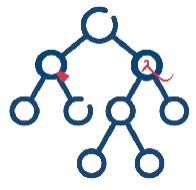
\includegraphics[height=1.0cm]{msca_logo.png}}%
    \end{center}

    \vspace{0.6cm}

    % Main title with Q logos on sides (with clickable links)
    \begin{center}
        \begin{minipage}{0.1\textwidth}
            \centering
            \href{https://quantlet.com}{
\includegraphics[height=1.1cm]{ql_logo.png}}
        \end{minipage}%
        \begin{minipage}{0.78\textwidth}
            \centering
            {\LARGE\bfseries\usebeamercolor[fg]{title}\inserttitle}

            \vspace{0.3cm}

            {\usebeamerfont{subtitle}\usebeamercolor[fg]{title}\insertsubtitle}
        \end{minipage}%
        \begin{minipage}{0.1\textwidth}
            \centering
            \href{https://quantinar.com}{
\includegraphics[height=1.1cm]{qr_logo.png}}
        \end{minipage}
    \end{center}

    \vspace{0.6cm}

    % Authors (left aligned)
    \hspace{0.5cm}{\usebeamerfont{author}\insertauthor}

    \vspace{0.3cm}

    % Institute/Affiliations (left aligned)
    \hspace{0.5cm}\begin{minipage}[t]{0.9\textwidth}
        \raggedright\small\insertinstitute
    \end{minipage}
}

%=============================================================================
% THEOREM ENVIRONMENTS
%=============================================================================
\theoremstyle{definition}
\setbeamertemplate{theorems}[numbered]
\ifdefined\sfmlang
\newtheorem{defn}{Definiție}
\newtheorem{thm}{Teoremă}
\newtheorem{prop}{Propoziție}
\newtheorem{rmk}{Observație}
\else
\newtheorem{defn}{Definition}
\newtheorem{thm}{Theorem}
\newtheorem{prop}{Proposition}
\newtheorem{rmk}{Remark}
\fi

%=============================================================================
% CENTRED MINIPAGE (no extra vertical space)
%=============================================================================
\newenvironment{cminipage}[1]{%
    \par\noindent\hfill\begin{minipage}{#1}\ignorespaces
}{%
    \end{minipage}\hfill\null\par
}

%=============================================================================
% CUSTOM COMMANDS
%=============================================================================
\newcommand{\E}{\mathbb{E}}
\newcommand{\Var}{\text{Var}}
\newcommand{\Cov}{\text{Cov}}
\newcommand{\Corr}{\text{Corr}}
\newcommand{\R}{\mathbb{R}}
\newcommand{\N}{\mathbb{N}}
\newcommand{\Z}{\mathbb{Z}}
\newcommand{\B}{\mathbf{B}}
\newcommand{\imark}{\textcolor{MainBlue}{\textbullet}}
\newcommand{\RMSE}{\text{RMSE}}
\newcommand{\MAE}{\text{MAE}}
\newcommand{\MAPE}{\text{MAPE}}

 se definește
%   \newcommand{\coursename}{Statistics of Financial Markets}      (EN)
%   \newcommand{\coursename}{Statistica piețelor financiare}       (RO)  și  \def\sfmlang{ro}
% Fișierele .tex se află în EN/Courses, EN/Seminars, RO/Cursuri, RO/Seminarii (două niveluri sub rădăcină).
% Deck-urile sînt generate de latex/build_chapterN.py / build_seminarN.py (vezi latex/sfm_build.py).

\documentclass[9pt, aspectratio=169, t]{beamer}
\providecommand{\coursename}{Statistics of Financial Markets}

% Ensure content fits on slides
\setbeamersize{text margin left=8mm, text margin right=8mm}

%=============================================================================
% THEME AND STYLE CONFIGURATION
%=============================================================================
\usetheme{default}
% Using default theme for clean header/footer control

% Color Palette (matching Redispatch PDF)
\definecolor{MainBlue}{RGB}{26, 58, 110}
\definecolor{AccentBlue}{RGB}{26, 58, 110}
\definecolor{IDAred}{RGB}{205, 0, 0}
\definecolor{DarkGray}{RGB}{51, 51, 51}
\definecolor{MediumGray}{RGB}{128, 128, 128}
\definecolor{LightGray}{RGB}{248, 248, 248}
\definecolor{VeryLightGray}{RGB}{235, 235, 235}
\definecolor{KeynoteGray}{RGB}{218, 218, 218}
\definecolor{SectionGray}{RGB}{120, 120, 120}
\definecolor{FooterGray}{RGB}{100, 100, 100}
\definecolor{Crimson}{RGB}{220, 53, 69}
\definecolor{Forest}{RGB}{46, 125, 50}
\definecolor{Amber}{RGB}{181, 133, 63}
\definecolor{Orange}{RGB}{230, 126, 34}
\definecolor{Purple}{RGB}{142, 68, 173}

% Gradient background (exact Keynote 315° gradient: white to RGB 218,218,218)
\setbeamertemplate{background}{%
    \begin{tikzpicture}[remember picture, overlay]
        \shade[shading=axis, shading angle=315,
        top color=white, bottom color=KeynoteGray]
        (current page.south west) rectangle (current page.north east);
    \end{tikzpicture}%
}
% Fallback solid color for compatibility
\setbeamercolor{background canvas}{bg=}

\setbeamercolor{palette primary}{bg=MainBlue, fg=white}
\setbeamercolor{palette secondary}{bg=MainBlue!85, fg=white}
\setbeamercolor{palette tertiary}{bg=MainBlue!70, fg=white}
\setbeamercolor{structure}{fg=MainBlue}
\setbeamercolor{title}{fg=IDAred}
\setbeamercolor{frametitle}{fg=IDAred, bg=}
\setbeamercolor{block title}{bg=MainBlue, fg=white}
\setbeamercolor{block body}{bg=VeryLightGray, fg=DarkGray}
\setbeamercolor{block title alerted}{bg=Crimson, fg=white}
\setbeamercolor{block body alerted}{bg=Crimson!8, fg=DarkGray}
\setbeamercolor{block title example}{bg=Forest, fg=white}
\setbeamercolor{block body example}{bg=Forest!8, fg=DarkGray}
\setbeamercolor{item}{fg=MainBlue}

% Footer colors (override Madrid theme blue)
\setbeamercolor{author in head/foot}{fg=FooterGray, bg=}
\setbeamercolor{title in head/foot}{fg=FooterGray, bg=}
\setbeamercolor{date in head/foot}{fg=FooterGray, bg=}
\setbeamercolor{section in head/foot}{fg=FooterGray, bg=}
\setbeamercolor{subsection in head/foot}{fg=FooterGray, bg=}

% Bullet styles (apply everywhere including blocks)
\setbeamertemplate{itemize item}{\color{MainBlue}$\boxdot$}
\setbeamertemplate{itemize subitem}{\color{MainBlue}$\blacktriangleright$}
\setbeamertemplate{itemize subsubitem}{\color{MainBlue}\tiny$\bullet$}
\setbeamertemplate{itemize/enumerate body begin}{\normalsize}
\setbeamertemplate{itemize/enumerate subbody begin}{\normalsize}

% Item spacing - compact style
\setlength{\leftmargini}{10pt}       % Level 1: minimal indent
\setlength{\leftmarginii}{10pt}      % Level 2: minimal additional indent
% Compact list spacing (zero extra space before/after lists in blocks)
\makeatletter
\def\@listi{\leftmargin\leftmargini \topsep 0pt \parsep 0pt \itemsep 0pt}
\def\@listii{\leftmargin\leftmarginii \topsep 0pt \parsep 0pt \itemsep 0pt}
\makeatother

\setbeamertemplate{navigation symbols}{}

%=============================================================================
% CUSTOM HEADLINE
%=============================================================================
\setbeamertemplate{headline}{%
    \vskip10pt%
    \hbox to \paperwidth{%
        \hskip0.5cm%
        {\small\color{FooterGray}\renewcommand{\hyperlink}[2]{##2}\insertsectionhead}%
        \hfill%
        \textcolor{FooterGray}{\small\insertframenumber}%
        \hskip0.5cm%
    }%
    \vskip4pt%
    {\color{FooterGray}\hrule height 0.4pt}%
}

%=============================================================================
% CUSTOM FOOTER
%=============================================================================
\usepackage{fontawesome5}

\setbeamertemplate{footline}{%
    {\color{FooterGray}\hrule height 0.4pt}%
    \vskip4pt%
    \hbox to \paperwidth{%
        \hskip0.5cm%
        \textcolor{FooterGray}{\small\coursename}%
        \hfill%
        \raisebox{-0.1em}{%
            \begin{tikzpicture}[x=0.08em, y=0.08em, line width=0.4pt]
                \draw[FooterGray] (0,3) -- (1,4) -- (2,3.5) -- (3,5) -- (4,4) -- (5,6) -- (6,5.5) -- (7,4) -- (8,5) -- (9,7) -- (10,6) -- (11,5) -- (12,6.5) -- (13,8) -- (14,7) -- (15,6) -- (16,7.5) -- (17,9) -- (18,8) -- (19,7) -- (20,8.5) -- (21,10) -- (22,9) -- (23,8) -- (24,9.5);
            \end{tikzpicture}%
        }%
        \hskip0.5cm%
    }%
    \vskip6pt%
}

%=============================================================================
% PACKAGES
%=============================================================================
\usepackage[utf8]{inputenc}
\DeclareUnicodeCharacter{03B1}{\ensuremath{\alpha}}
\usepackage[T1]{fontenc}
\usepackage{amsmath, amssymb, amsthm}
\usepackage{mathtools}
\usepackage{bm}
\usepackage{tikz}
\usetikzlibrary{arrows.meta, positioning, shapes, calc, decorations.pathreplacing, shadings}
\usepackage{booktabs}
\usepackage{multirow}
\usepackage{array}
\usepackage{graphicx}
\usepackage{hyperref}
\usepackage{colortbl}
\usepackage{listings}
\lstset{language=Python, basicstyle=\ttfamily\scriptsize, keywordstyle=\color{MainBlue}\bfseries,
  commentstyle=\color{Forest}, stringstyle=\color{Crimson}, breaklines=true,
  frame=none, backgroundcolor=\color{VeryLightGray}, xleftmargin=2mm}
\hypersetup{colorlinks=true, linkcolor=MainBlue, urlcolor=MainBlue}
\graphicspath{{../../logos/}{../../charts/}{../../photos/}}
\usepackage{xcolor}
\hfuzz=2pt  % Suppress tiny overfull warnings (<2pt)
\vfuzz=2pt  % Suppress tiny vertical overfull warnings (<2pt)

%=============================================================================
% QUANTLET COMMANDS
%   \quantlet{<displayed name>}{<url>}       (generic, compatible with the older SFM decks)
%   \sfmquantlet{Ch_05}{SFM_ch5_garch}       -> https://github.com/danpele/SFM/tree/main/Quantlets/Ch_05/SFM_ch5_garch
%   \qlurl{<folder>} is defined per chapter by the generator (Quantlets/Ch_NN/<folder>)
%=============================================================================
\newcommand{\sfmrepo}{https://github.com/danpele/SFM}
\newcommand{\sfmqlbase}{https://github.com/danpele/SFM/tree/main/Quantlets}
\newcommand{\quantlet}[2]{%
    \hfill\href{#2}{%
        \raisebox{-0.15em}{
\includegraphics[height=0.7em]{ql_logo.png}}%
        \textcolor{MainBlue}{\tiny\ #1}%
    }%
}
\newcommand{\sfmquantlet}[2]{\quantlet{\detokenize{#2}}{\sfmqlbase/#1/#2}}

%=============================================================================
% NOTEBOOKS (Google Colab)
%   \colaburl{notebooks/EN/chapter5_seminar_notebook.ipynb} -> the Colab link of a file in the SFM repo
%   \nb: the chapter notebook (each seminar deck redefines it with \renewcommand)
%=============================================================================
\newcommand{\colaburl}[1]{https://colab.research.google.com/github/danpele/SFM/blob/main/#1}
\newcommand{\nb}{https://colab.research.google.com/github/danpele/SFM/tree/main/notebooks/EN}
\newcommand{\nbname}{notebooks/EN}

%=============================================================================
% SLIDE HELPERS (used by the generators; the same as in MFM)
%=============================================================================
% local font size for list bodies (the preamble forces \normalsize)
\newcommand{\itemsize}[1]{\setbeamertemplate{itemize/enumerate body begin}{#1}\setbeamertemplate{itemize/enumerate subbody begin}{#1}}
\newcommand{\intitle}[1]{{\hypersetup{urlcolor=white}#1}}   % white links inside coloured title bars
\newcommand{\imgcap}[1]{{\scriptsize #1}\\[0.5mm]}          % caption under a photo
\newcommand{\imgcredit}[2]{{\tiny\color{FooterGray}\href{#1}{#2}}}   % image credit: source URL, author/licence
\newcommand{\aiprompt}[1]{{\ttfamily\color{MainBlue}#1}}     % a prompt to an AI assistant

%=============================================================================
% SEMINARS: student version by default; the instructor wrapper *_solutions.tex sets \solutionstrue
%=============================================================================
\makeatletter\@ifundefined{ifsolutions}{\expandafter\newif\csname ifsolutions\endcsname}{}\makeatother
\newcommand{\solonly}[1]{\ifsolutions #1\fi}
\newcommand{\propsub}{\ifsolutions\else\framesubtitle{\ifdefined\sfmlang Rezolvarea se discută la seminar\else Solution discussed in class\fi}\fi}

%=============================================================================
% APPENDIX AND CHAPTER LINKS (latex/appendix_links.py writes the calls; it also re-declares these
% macros before \begin{document}, so the decks compile with or without this preamble block)
%=============================================================================
\providecommand{\sfmapplink}[3]{\hypertarget{#2}{}\hyperlink{#1}{\beamergotobutton{#3}}}
\providecommand{\sfmappback}[2]{\begin{tikzpicture}[remember picture,overlay]\node[anchor=south east] at ([xshift=-3mm,yshift=7mm]current page.south east){\hyperlink{#1}{\beamerreturnbutton{#2}}};\end{tikzpicture}}
\providecommand{\sfmchlink}[2]{\href{#1}{#2}}
\providecommand{\sfmchlinkt}[2]{\href{#1}{\usebeamercolor[fg]{frametitle}#2}}

%=============================================================================
% QUANTINAR COMMAND: link către un curs Quantinar (subiecte avansate)
%=============================================================================
\newcommand{\quantinar}[2]{%
    \href{#2}{%
        \raisebox{-0.15em}{
\includegraphics[height=0.8em]{qr_logo.png}}%
        \textcolor{MainBlue}{\scriptsize\ #1}%
    }%
}

%=============================================================================
% CUSTOM TITLE PAGE
%=============================================================================
\defbeamertemplate*{title page}{hybrid}[1][]
{
    \vspace{0.2cm}
    % Logos row - top header (with clickable links)
    \begin{center}
        \href{https://www.ase.ro}{
\includegraphics[height=1.0cm]{ase_logo.png}}\hspace{0.3cm}%
        \href{https://theida.net}{
\includegraphics[height=1.0cm]{ida_logo.png}}\hspace{0.3cm}%
        \href{https://blockchain-research-center.com}{
\includegraphics[height=1.0cm]{brc_logo.png}}\hspace{0.3cm}%
        \href{https://www.ai4efin.ase.ro}{
\includegraphics[height=1.0cm]{ai4efin_logo.png}}\hspace{0.3cm}%
        \href{https://ipe.ro/new}{
\includegraphics[height=1.0cm]{acad_logo.png}}\hspace{0.3cm}%
        \href{https://www.digital-finance-msca.com}{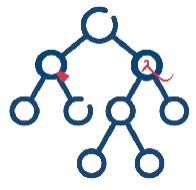
\includegraphics[height=1.0cm]{msca_logo.png}}%
    \end{center}

    \vspace{0.6cm}

    % Main title with Q logos on sides (with clickable links)
    \begin{center}
        \begin{minipage}{0.1\textwidth}
            \centering
            \href{https://quantlet.com}{
\includegraphics[height=1.1cm]{ql_logo.png}}
        \end{minipage}%
        \begin{minipage}{0.78\textwidth}
            \centering
            {\LARGE\bfseries\usebeamercolor[fg]{title}\inserttitle}

            \vspace{0.3cm}

            {\usebeamerfont{subtitle}\usebeamercolor[fg]{title}\insertsubtitle}
        \end{minipage}%
        \begin{minipage}{0.1\textwidth}
            \centering
            \href{https://quantinar.com}{
\includegraphics[height=1.1cm]{qr_logo.png}}
        \end{minipage}
    \end{center}

    \vspace{0.6cm}

    % Authors (left aligned)
    \hspace{0.5cm}{\usebeamerfont{author}\insertauthor}

    \vspace{0.3cm}

    % Institute/Affiliations (left aligned)
    \hspace{0.5cm}\begin{minipage}[t]{0.9\textwidth}
        \raggedright\small\insertinstitute
    \end{minipage}
}

%=============================================================================
% THEOREM ENVIRONMENTS
%=============================================================================
\theoremstyle{definition}
\setbeamertemplate{theorems}[numbered]
\ifdefined\sfmlang
\newtheorem{defn}{Definiție}
\newtheorem{thm}{Teoremă}
\newtheorem{prop}{Propoziție}
\newtheorem{rmk}{Observație}
\else
\newtheorem{defn}{Definition}
\newtheorem{thm}{Theorem}
\newtheorem{prop}{Proposition}
\newtheorem{rmk}{Remark}
\fi

%=============================================================================
% CENTRED MINIPAGE (no extra vertical space)
%=============================================================================
\newenvironment{cminipage}[1]{%
    \par\noindent\hfill\begin{minipage}{#1}\ignorespaces
}{%
    \end{minipage}\hfill\null\par
}

%=============================================================================
% CUSTOM COMMANDS
%=============================================================================
\newcommand{\E}{\mathbb{E}}
\newcommand{\Var}{\text{Var}}
\newcommand{\Cov}{\text{Cov}}
\newcommand{\Corr}{\text{Corr}}
\newcommand{\R}{\mathbb{R}}
\newcommand{\N}{\mathbb{N}}
\newcommand{\Z}{\mathbb{Z}}
\newcommand{\B}{\mathbf{B}}
\newcommand{\imark}{\textcolor{MainBlue}{\textbullet}}
\newcommand{\RMSE}{\text{RMSE}}
\newcommand{\MAE}{\text{MAE}}
\newcommand{\MAPE}{\text{MAPE}}

 se definește
%   \newcommand{\coursename}{Statistics of Financial Markets}      (EN)
%   \newcommand{\coursename}{Statistica piețelor financiare}       (RO)  și  \def\sfmlang{ro}
% Fișierele .tex se află în EN/Courses, EN/Seminars, RO/Cursuri, RO/Seminarii (două niveluri sub rădăcină).
% Deck-urile sînt generate de latex/build_chapterN.py / build_seminarN.py (vezi latex/sfm_build.py).

\documentclass[9pt, aspectratio=169, t]{beamer}
\providecommand{\coursename}{Statistics of Financial Markets}

% Ensure content fits on slides
\setbeamersize{text margin left=8mm, text margin right=8mm}

%=============================================================================
% THEME AND STYLE CONFIGURATION
%=============================================================================
\usetheme{default}
% Using default theme for clean header/footer control

% Color Palette (matching Redispatch PDF)
\definecolor{MainBlue}{RGB}{26, 58, 110}
\definecolor{AccentBlue}{RGB}{26, 58, 110}
\definecolor{IDAred}{RGB}{205, 0, 0}
\definecolor{DarkGray}{RGB}{51, 51, 51}
\definecolor{MediumGray}{RGB}{128, 128, 128}
\definecolor{LightGray}{RGB}{248, 248, 248}
\definecolor{VeryLightGray}{RGB}{235, 235, 235}
\definecolor{KeynoteGray}{RGB}{218, 218, 218}
\definecolor{SectionGray}{RGB}{120, 120, 120}
\definecolor{FooterGray}{RGB}{100, 100, 100}
\definecolor{Crimson}{RGB}{220, 53, 69}
\definecolor{Forest}{RGB}{46, 125, 50}
\definecolor{Amber}{RGB}{181, 133, 63}
\definecolor{Orange}{RGB}{230, 126, 34}
\definecolor{Purple}{RGB}{142, 68, 173}

% Gradient background (exact Keynote 315° gradient: white to RGB 218,218,218)
\setbeamertemplate{background}{%
    \begin{tikzpicture}[remember picture, overlay]
        \shade[shading=axis, shading angle=315,
        top color=white, bottom color=KeynoteGray]
        (current page.south west) rectangle (current page.north east);
    \end{tikzpicture}%
}
% Fallback solid color for compatibility
\setbeamercolor{background canvas}{bg=}

\setbeamercolor{palette primary}{bg=MainBlue, fg=white}
\setbeamercolor{palette secondary}{bg=MainBlue!85, fg=white}
\setbeamercolor{palette tertiary}{bg=MainBlue!70, fg=white}
\setbeamercolor{structure}{fg=MainBlue}
\setbeamercolor{title}{fg=IDAred}
\setbeamercolor{frametitle}{fg=IDAred, bg=}
\setbeamercolor{block title}{bg=MainBlue, fg=white}
\setbeamercolor{block body}{bg=VeryLightGray, fg=DarkGray}
\setbeamercolor{block title alerted}{bg=Crimson, fg=white}
\setbeamercolor{block body alerted}{bg=Crimson!8, fg=DarkGray}
\setbeamercolor{block title example}{bg=Forest, fg=white}
\setbeamercolor{block body example}{bg=Forest!8, fg=DarkGray}
\setbeamercolor{item}{fg=MainBlue}

% Footer colors (override Madrid theme blue)
\setbeamercolor{author in head/foot}{fg=FooterGray, bg=}
\setbeamercolor{title in head/foot}{fg=FooterGray, bg=}
\setbeamercolor{date in head/foot}{fg=FooterGray, bg=}
\setbeamercolor{section in head/foot}{fg=FooterGray, bg=}
\setbeamercolor{subsection in head/foot}{fg=FooterGray, bg=}

% Bullet styles (apply everywhere including blocks)
\setbeamertemplate{itemize item}{\color{MainBlue}$\boxdot$}
\setbeamertemplate{itemize subitem}{\color{MainBlue}$\blacktriangleright$}
\setbeamertemplate{itemize subsubitem}{\color{MainBlue}\tiny$\bullet$}
\setbeamertemplate{itemize/enumerate body begin}{\normalsize}
\setbeamertemplate{itemize/enumerate subbody begin}{\normalsize}

% Item spacing - compact style
\setlength{\leftmargini}{10pt}       % Level 1: minimal indent
\setlength{\leftmarginii}{10pt}      % Level 2: minimal additional indent
% Compact list spacing (zero extra space before/after lists in blocks)
\makeatletter
\def\@listi{\leftmargin\leftmargini \topsep 0pt \parsep 0pt \itemsep 0pt}
\def\@listii{\leftmargin\leftmarginii \topsep 0pt \parsep 0pt \itemsep 0pt}
\makeatother

\setbeamertemplate{navigation symbols}{}

%=============================================================================
% CUSTOM HEADLINE
%=============================================================================
\setbeamertemplate{headline}{%
    \vskip10pt%
    \hbox to \paperwidth{%
        \hskip0.5cm%
        {\small\color{FooterGray}\renewcommand{\hyperlink}[2]{##2}\insertsectionhead}%
        \hfill%
        \textcolor{FooterGray}{\small\insertframenumber}%
        \hskip0.5cm%
    }%
    \vskip4pt%
    {\color{FooterGray}\hrule height 0.4pt}%
}

%=============================================================================
% CUSTOM FOOTER
%=============================================================================
\usepackage{fontawesome5}

\setbeamertemplate{footline}{%
    {\color{FooterGray}\hrule height 0.4pt}%
    \vskip4pt%
    \hbox to \paperwidth{%
        \hskip0.5cm%
        \textcolor{FooterGray}{\small\coursename}%
        \hfill%
        \raisebox{-0.1em}{%
            \begin{tikzpicture}[x=0.08em, y=0.08em, line width=0.4pt]
                \draw[FooterGray] (0,3) -- (1,4) -- (2,3.5) -- (3,5) -- (4,4) -- (5,6) -- (6,5.5) -- (7,4) -- (8,5) -- (9,7) -- (10,6) -- (11,5) -- (12,6.5) -- (13,8) -- (14,7) -- (15,6) -- (16,7.5) -- (17,9) -- (18,8) -- (19,7) -- (20,8.5) -- (21,10) -- (22,9) -- (23,8) -- (24,9.5);
            \end{tikzpicture}%
        }%
        \hskip0.5cm%
    }%
    \vskip6pt%
}

%=============================================================================
% PACKAGES
%=============================================================================
\usepackage[utf8]{inputenc}
\DeclareUnicodeCharacter{03B1}{\ensuremath{\alpha}}
\usepackage[T1]{fontenc}
\usepackage{amsmath, amssymb, amsthm}
\usepackage{mathtools}
\usepackage{bm}
\usepackage{tikz}
\usetikzlibrary{arrows.meta, positioning, shapes, calc, decorations.pathreplacing, shadings}
\usepackage{booktabs}
\usepackage{multirow}
\usepackage{array}
\usepackage{graphicx}
\usepackage{hyperref}
\usepackage{colortbl}
\usepackage{listings}
\lstset{language=Python, basicstyle=\ttfamily\scriptsize, keywordstyle=\color{MainBlue}\bfseries,
  commentstyle=\color{Forest}, stringstyle=\color{Crimson}, breaklines=true,
  frame=none, backgroundcolor=\color{VeryLightGray}, xleftmargin=2mm}
\hypersetup{colorlinks=true, linkcolor=MainBlue, urlcolor=MainBlue}
\graphicspath{{../../logos/}{../../charts/}{../../photos/}}
\usepackage{xcolor}
\hfuzz=2pt  % Suppress tiny overfull warnings (<2pt)
\vfuzz=2pt  % Suppress tiny vertical overfull warnings (<2pt)

%=============================================================================
% QUANTLET COMMANDS
%   \quantlet{<displayed name>}{<url>}       (generic, compatible with the older SFM decks)
%   \sfmquantlet{Ch_05}{SFM_ch5_garch}       -> https://github.com/danpele/SFM/tree/main/Quantlets/Ch_05/SFM_ch5_garch
%   \qlurl{<folder>} is defined per chapter by the generator (Quantlets/Ch_NN/<folder>)
%=============================================================================
\newcommand{\sfmrepo}{https://github.com/danpele/SFM}
\newcommand{\sfmqlbase}{https://github.com/danpele/SFM/tree/main/Quantlets}
\newcommand{\quantlet}[2]{%
    \hfill\href{#2}{%
        \raisebox{-0.15em}{
\includegraphics[height=0.7em]{ql_logo.png}}%
        \textcolor{MainBlue}{\tiny\ #1}%
    }%
}
\newcommand{\sfmquantlet}[2]{\quantlet{\detokenize{#2}}{\sfmqlbase/#1/#2}}

%=============================================================================
% NOTEBOOKS (Google Colab)
%   \colaburl{notebooks/EN/chapter5_seminar_notebook.ipynb} -> the Colab link of a file in the SFM repo
%   \nb: the chapter notebook (each seminar deck redefines it with \renewcommand)
%=============================================================================
\newcommand{\colaburl}[1]{https://colab.research.google.com/github/danpele/SFM/blob/main/#1}
\newcommand{\nb}{https://colab.research.google.com/github/danpele/SFM/tree/main/notebooks/EN}
\newcommand{\nbname}{notebooks/EN}

%=============================================================================
% SLIDE HELPERS (used by the generators; the same as in MFM)
%=============================================================================
% local font size for list bodies (the preamble forces \normalsize)
\newcommand{\itemsize}[1]{\setbeamertemplate{itemize/enumerate body begin}{#1}\setbeamertemplate{itemize/enumerate subbody begin}{#1}}
\newcommand{\intitle}[1]{{\hypersetup{urlcolor=white}#1}}   % white links inside coloured title bars
\newcommand{\imgcap}[1]{{\scriptsize #1}\\[0.5mm]}          % caption under a photo
\newcommand{\imgcredit}[2]{{\tiny\color{FooterGray}\href{#1}{#2}}}   % image credit: source URL, author/licence
\newcommand{\aiprompt}[1]{{\ttfamily\color{MainBlue}#1}}     % a prompt to an AI assistant

%=============================================================================
% SEMINARS: student version by default; the instructor wrapper *_solutions.tex sets \solutionstrue
%=============================================================================
\makeatletter\@ifundefined{ifsolutions}{\expandafter\newif\csname ifsolutions\endcsname}{}\makeatother
\newcommand{\solonly}[1]{\ifsolutions #1\fi}
\newcommand{\propsub}{\ifsolutions\else\framesubtitle{\ifdefined\sfmlang Rezolvarea se discută la seminar\else Solution discussed in class\fi}\fi}

%=============================================================================
% APPENDIX AND CHAPTER LINKS (latex/appendix_links.py writes the calls; it also re-declares these
% macros before \begin{document}, so the decks compile with or without this preamble block)
%=============================================================================
\providecommand{\sfmapplink}[3]{\hypertarget{#2}{}\hyperlink{#1}{\beamergotobutton{#3}}}
\providecommand{\sfmappback}[2]{\begin{tikzpicture}[remember picture,overlay]\node[anchor=south east] at ([xshift=-3mm,yshift=7mm]current page.south east){\hyperlink{#1}{\beamerreturnbutton{#2}}};\end{tikzpicture}}
\providecommand{\sfmchlink}[2]{\href{#1}{#2}}
\providecommand{\sfmchlinkt}[2]{\href{#1}{\usebeamercolor[fg]{frametitle}#2}}

%=============================================================================
% QUANTINAR COMMAND: link către un curs Quantinar (subiecte avansate)
%=============================================================================
\newcommand{\quantinar}[2]{%
    \href{#2}{%
        \raisebox{-0.15em}{
\includegraphics[height=0.8em]{qr_logo.png}}%
        \textcolor{MainBlue}{\scriptsize\ #1}%
    }%
}

%=============================================================================
% CUSTOM TITLE PAGE
%=============================================================================
\defbeamertemplate*{title page}{hybrid}[1][]
{
    \vspace{0.2cm}
    % Logos row - top header (with clickable links)
    \begin{center}
        \href{https://www.ase.ro}{
\includegraphics[height=1.0cm]{ase_logo.png}}\hspace{0.3cm}%
        \href{https://theida.net}{
\includegraphics[height=1.0cm]{ida_logo.png}}\hspace{0.3cm}%
        \href{https://blockchain-research-center.com}{
\includegraphics[height=1.0cm]{brc_logo.png}}\hspace{0.3cm}%
        \href{https://www.ai4efin.ase.ro}{
\includegraphics[height=1.0cm]{ai4efin_logo.png}}\hspace{0.3cm}%
        \href{https://ipe.ro/new}{
\includegraphics[height=1.0cm]{acad_logo.png}}\hspace{0.3cm}%
        \href{https://www.digital-finance-msca.com}{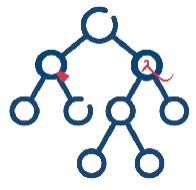
\includegraphics[height=1.0cm]{msca_logo.png}}%
    \end{center}

    \vspace{0.6cm}

    % Main title with Q logos on sides (with clickable links)
    \begin{center}
        \begin{minipage}{0.1\textwidth}
            \centering
            \href{https://quantlet.com}{
\includegraphics[height=1.1cm]{ql_logo.png}}
        \end{minipage}%
        \begin{minipage}{0.78\textwidth}
            \centering
            {\LARGE\bfseries\usebeamercolor[fg]{title}\inserttitle}

            \vspace{0.3cm}

            {\usebeamerfont{subtitle}\usebeamercolor[fg]{title}\insertsubtitle}
        \end{minipage}%
        \begin{minipage}{0.1\textwidth}
            \centering
            \href{https://quantinar.com}{
\includegraphics[height=1.1cm]{qr_logo.png}}
        \end{minipage}
    \end{center}

    \vspace{0.6cm}

    % Authors (left aligned)
    \hspace{0.5cm}{\usebeamerfont{author}\insertauthor}

    \vspace{0.3cm}

    % Institute/Affiliations (left aligned)
    \hspace{0.5cm}\begin{minipage}[t]{0.9\textwidth}
        \raggedright\small\insertinstitute
    \end{minipage}
}

%=============================================================================
% THEOREM ENVIRONMENTS
%=============================================================================
\theoremstyle{definition}
\setbeamertemplate{theorems}[numbered]
\ifdefined\sfmlang
\newtheorem{defn}{Definiție}
\newtheorem{thm}{Teoremă}
\newtheorem{prop}{Propoziție}
\newtheorem{rmk}{Observație}
\else
\newtheorem{defn}{Definition}
\newtheorem{thm}{Theorem}
\newtheorem{prop}{Proposition}
\newtheorem{rmk}{Remark}
\fi

%=============================================================================
% CENTRED MINIPAGE (no extra vertical space)
%=============================================================================
\newenvironment{cminipage}[1]{%
    \par\noindent\hfill\begin{minipage}{#1}\ignorespaces
}{%
    \end{minipage}\hfill\null\par
}

%=============================================================================
% CUSTOM COMMANDS
%=============================================================================
\newcommand{\E}{\mathbb{E}}
\newcommand{\Var}{\text{Var}}
\newcommand{\Cov}{\text{Cov}}
\newcommand{\Corr}{\text{Corr}}
\newcommand{\R}{\mathbb{R}}
\newcommand{\N}{\mathbb{N}}
\newcommand{\Z}{\mathbb{Z}}
\newcommand{\B}{\mathbf{B}}
\newcommand{\imark}{\textcolor{MainBlue}{\textbullet}}
\newcommand{\RMSE}{\text{RMSE}}
\newcommand{\MAE}{\text{MAE}}
\newcommand{\MAPE}{\text{MAPE}}



\newcommand{\qlurl}[1]{https://github.com/danpele/SFM/tree/main/Quantlets/Ch_14/#1}

% Clickable citations (DOIs verified via Crossref)

\newcommand{\refNakamoto}{\href{https://bitcoin.org/bitcoin.pdf}{Nakamoto (2008)}}
\newcommand{\refButerin}{\href{https://ethereum.org/en/whitepaper/}{Buterin (2014)}}
\newcommand{\refMerge}{\href{https://ethereum.org/en/roadmap/merge/}{ethereum.org: The Merge}}
\newcommand{\refLT}{\href{https://doi.org/10.1093/rfs/hhaa113}{Liu \& Tsyvinski (2021)}}
\newcommand{\refLTW}{\href{https://doi.org/10.1111/jofi.13119}{Liu, Tsyvinski \& Wu (2022)}}
\newcommand{\refGS}{\href{https://doi.org/10.1111/jofi.12903}{Griffin \& Shams (2020)}}
\newcommand{\refMS}{\href{https://doi.org/10.1016/j.jfineco.2019.07.001}{Makarov \& Schoar (2020)}}
\newcommand{\refGorton}{\href{https://doi.org/10.3386/w30796}{Gorton et al.\ (2022)}}
\newcommand{\refGZ}{\href{https://doi.org/10.2139/ssrn.3888752}{Gorton \& Zhang (2021)}}
\newcommand{\refLVN}{\href{https://doi.org/10.1016/j.jimonfin.2022.102777}{Lyons \& Viswanath-Natraj (2023)}}
\newcommand{\refLMS}{\href{https://doi.org/10.3386/w31160}{Liu, Makarov \& Schoar (2023)}}
\newcommand{\refMZZ}{\href{https://doi.org/10.3386/w33882}{Ma, Zeng \& Zhang (2025)}}
\newcommand{\refUrquhart}{\href{https://doi.org/10.1016/j.econlet.2016.09.019}{Urquhart (2016)}}
\newcommand{\refNC}{\href{https://doi.org/10.1016/j.econlet.2016.10.033}{Nadarajah \& Chu (2017)}}
\newcommand{\refTL}{\href{https://doi.org/10.1016/j.frl.2019.101382}{Tran \& Leirvik (2020)}}
\newcommand{\refCF}{\href{https://doi.org/10.1016/j.econlet.2015.02.029}{Cheah \& Fry (2015)}}
\newcommand{\refKatsiampa}{\href{https://doi.org/10.1016/j.econlet.2017.06.023}{Katsiampa (2017)}}
\newcommand{\refBL}{\href{https://doi.org/10.1111/j.1540-6288.2010.00244.x}{Baur \& Lucey (2010)}}
\newcommand{\refBHL}{\href{https://doi.org/10.1016/j.intfin.2017.12.004}{Baur, Hong \& Lee (2018)}}
\newcommand{\refCP}{\href{https://doi.org/10.1016/j.frl.2018.11.012}{Caporale \& Plastun (2019)}}
\newcommand{\refGHMO}{\href{https://doi.org/10.1016/j.jmoneco.2017.12.004}{Gandal et al.\ (2018)}}
\newcommand{\refHill}{\href{https://doi.org/10.1214/aos/1176343247}{Hill (1975)}}
\newcommand{\refBoll}{\href{https://doi.org/10.1016/0304-4076(86)90063-1}{Bollerslev (1986)}}
\newcommand{\refLM}{\href{https://doi.org/10.1093/rfs/1.1.41}{Lo \& MacKinlay (1988)}}
\newcommand{\refFama}{\href{https://doi.org/10.2307/2325486}{Fama (1970)}}
\newcommand{\refJLS}{\href{https://doi.org/10.1142/S0219024900000115}{Johansen, Ledoit \& Sornette (2000)}}
\newcommand{\refTH}{\href{https://doi.org/10.1016/j.jempfin.2018.08.004}{Trimborn \& Härdle (2018)}}
\newcommand{\refHHR}{\href{https://doi.org/10.1093/jjfinec/nbz033}{Härdle, Harvey \& Reule (2020)}}
\newcommand{\refFHH}{\href{https://doi.org/10.1007/978-3-030-13751-9}{Franke, Härdle \& Hafner (2019)}}
\newcommand{\refKupiec}{\href{https://doi.org/10.3905/jod.1995.407942}{Kupiec (1995)}}
\newcommand{\refWang}{\href{https://doi.org/10.1038/s41586-023-06221-2}{Wang et al.\ (2023)}}
\newcommand{\refPeleA}{\href{https://doi.org/10.1080/1351847X.2021.1960403}{Pele et al.\ (2023)}}
\newcommand{\refPeleB}{\href{https://doi.org/10.3390/e21020102}{Pele \& Mazurencu-Marinescu-Pele (2019)}}
\newcommand{\refMiCA}{\href{https://eur-lex.europa.eu/eli/reg/2023/1114/oj}{Regulation (EU) 2023/1114 (MiCA)}}
\newcommand{\refESMA}{\href{https://www.esma.europa.eu/esmas-activities/digital-finance-and-innovation/markets-crypto-assets-regulation-mica}{ESMA: MiCA}}
\newcommand{\refGENIUS}{\href{https://www.govinfo.gov/app/details/PLAW-119publ27}{GENIUS Act, Public Law 119-27}}
\newcommand{\refSEC}{\href{https://www.sec.gov/newsroom/speeches-statements/gensler-statement-spot-bitcoin-011023}{SEC (2024)}}
\newcommand{\refFed}{\href{https://www.federalreserve.gov/newsevents/pressreleases/monetary20230312b.htm}{Treasury, Federal Reserve and FDIC (2023)}}
\newcommand{\refFDIC}{\href{https://www.fdic.gov/news/press-releases/2023/pr23016.html}{FDIC (2023)}}
\newcommand{\refDL}{\href{https://api-docs.defillama.com/}{DefiLlama}}

\title[Statistics of Financial Markets]{Statistics of Financial Markets}
\subtitle{Chapter 14: Crypto assets}
\author[D.T. Pele]{Daniel Traian PELE}
\institute{Bucharest University of Economic Studies\\
IDA Institute Digital Assets\\
Blockchain Research Center\\
AI4EFin Artificial Intelligence for Energy Finance\\
Romanian Academy, Institute for Economic Forecasting\\
MSCA Digital Finance}
\date{}

%=============================================================================
\providecommand{\sfmapplink}[3]{\hypertarget{#2}{}\hyperlink{#1}{\beamergotobutton{#3}}}  % APPLINKS-MACROS
\providecommand{\sfmappback}[2]{\begin{tikzpicture}[remember picture,overlay]\node[anchor=south east] at ([xshift=-3mm,yshift=7mm]current page.south east){\hyperlink{#1}{\beamerreturnbutton{#2}}};\end{tikzpicture}}  % APPLINKS-MACROS
\providecommand{\sfmchlink}[2]{\href{#1}{#2}}  % APPLINKS-MACROS
\providecommand{\sfmchlinkt}[2]{\href{#1}{\usebeamercolor[fg]{frametitle}#2}}  % APPLINKS-MACROS
\begin{document}
%=============================================================================

{
\setbeamertemplate{headline}{}
\setbeamertemplate{footline}{}
\begin{frame}[noframenumbering]
    \titlepage
\end{frame}
}
% BEGIN-ACRONYMS (generat de latex/acronyms.py; nu editati manual)
\begin{frame}{Acronyms used in this material (1/2)}
\setbeamertemplate{itemize/enumerate body begin}{\tiny}
\begin{columns}[T]
\begin{column}{0.49\textwidth}
\begin{itemize}\setlength{\itemsep}{0pt}
    \item \textbf{ACF}: Autocorrelation Function
    \item \textbf{AI}: Artificial Intelligence
    \item \textbf{AIC}: Akaike Information Criterion
    \item \textbf{API}: Application Programming Interface
    \item \textbf{AR}: AutoRegressive (model); in event studies: Abnormal Return
    \item \textbf{ATM}: Automated Teller Machine
    \item \textbf{CI}: Confidence Interval
    \item \textbf{COVID-19}: COronaVIrus Disease 2019
    \item \textbf{CRIX}: CRypto IndeX
    \item \textbf{DAI}: Dai (stablecoin of the MakerDAO protocol)
    \item \textbf{EODHD}: EOD Historical Data (market-data provider)
    \item \textbf{ES}: Expected Shortfall
    \item \textbf{ETF}: Exchange-Traded Fund
\end{itemize}
\end{column}
\begin{column}{0.49\textwidth}
\begin{itemize}\setlength{\itemsep}{0pt}
    \item \textbf{EWMA}: Exponentially Weighted Moving Average
    \item \textbf{FTX}: FTX Trading Ltd. (crypto exchange, bankrupt in November 2022)
    \item \textbf{GARCH}: Generalised AutoRegressive Conditional Heteroskedasticity
    \item \textbf{GENIUS}: Guiding and Establishing National Innovation for U.S. Stablecoins (Act)
    \item \textbf{GJR}: Glosten–Jagannathan–Runkle (asymmetric GARCH)
    \item \textbf{HAC}: Heteroskedasticity and Autocorrelation Consistent (standard errors)
    \item \textbf{HS}: Historical Simulation
    \item \textbf{IGARCH}: Integrated GARCH
    \item \textbf{LPPL}: Log-Periodic Power Law
    \item \textbf{LUNA}: Luna (token of the Terra blockchain)
    \item \textbf{SEC}: Securities and Exchange Commission
    \item \textbf{SHA-256}: Secure Hash Algorithm, 256 bits
    \item \textbf{SVB}: Silicon Valley Bank
\end{itemize}
\end{column}
\end{columns}
\end{frame}
\begin{frame}{Acronyms used in this material (2/2)}
\setbeamertemplate{itemize/enumerate body begin}{\tiny}
\begin{columns}[T]
\begin{column}{0.49\textwidth}
\begin{itemize}\setlength{\itemsep}{0pt}
    \item \textbf{US}: United States
    \item \textbf{USDC}: USD Coin
    \item \textbf{UST}: TerraUSD
    \item \textbf{UTC}: Coordinated Universal Time (Temps Universel Coordonné)
    \item \textbf{VR}: Variance Ratio
\end{itemize}
\end{column}
\begin{column}{0.49\textwidth}
\end{column}
\end{columns}
\end{frame}
% END-ACRONYMS

\begin{frame}{Today's Question and Route}
\itemsize{\small}
\begin{itemize}
    \item \textbf{Question}: do the statistical tools of \sfmchlink{https://danpele.github.io/SFM/EN/Courses/chapter2_classical_distributions_stylised_facts.pdf}{Chapters 2}--\sfmchlink{https://danpele.github.io/SFM/EN/Courses/chapter10_var_es_backtesting.pdf}{10} work for a market that never closes, has no cash flows and can lose 80\% of its value?
    \begin{itemize}
        \item the answer is a statistics-of-markets view of crypto assets, not a course in cryptography
    \end{itemize}
    \item \textbf{Route} of the chapter
    \begin{itemize}
        \item Bitcoin and Ethereum: blockchain, proof of work and of stake, the halving
        \item crypto as an asset class: annualisation with 365 days, tails, volatility clustering, GARCH, efficiency, the weekend
        \item correlation with equities and gold; bubbles and drawdowns; the spot Bitcoin ETFs of 2024
        \item stablecoins: types, supply, peg deviations, USDC in March 2023, the collapse of TerraUSD; regulation; VaR 1\% and ES 2.5\%
    \end{itemize}
\end{itemize}
\end{frame}

\begin{frame}{Learning Outcomes}
\itemsize{\small}
\begin{itemize}
    \item Explain how a blockchain records ownership, why mining costs energy and how the Bitcoin supply follows from the halving rule
    \item Annualise crypto returns and volatilities with the actual frequency (365 days) and say what goes wrong with 252
    \item Estimate the tail index, a GARCH(1,1)-t model and variance-ratio tests for Bitcoin and compare them with the S\&P 500
    \item Measure the correlation of crypto with equities and gold over time, and the drawdowns of a crypto asset
    \item Describe the three types of stablecoins, measure a peg deviation in basis points and read a depeg episode
    \item Compute VaR 1\% and ES 2.5\% of a crypto position and backtest them
\end{itemize}
\end{frame}

\begin{frame}{Reading and Tools}
\itemsize{\small}
\begin{itemize}
    \item Textbook: \refFHH, Ch.~23 (cryptocurrencies)
    \begin{itemize}
        \item surveys: \refHHR; crypto index CRIX: \refTH
        \item risks and returns: \refLT; stablecoins: \refGorton, \refLVN
    \end{itemize}
    \item Python Quantlets of this chapter: \href{https://github.com/danpele/SFM/tree/main/Quantlets/Ch_14}{Quantlets/Ch\_14}
    \begin{itemize}
        \item daily data from EODHD (crypto close, 7 days a week); stablecoin supply from \refDL
    \end{itemize}
    \item Lecture notebook: \href{\colaburl{notebooks/EN/chapter14_lecture_notebook.ipynb}}{open in Google Colab}
    \item Video courses: \quantinar{Introduction to Blockchain and Cryptocurrencies}{https://quantinar.com/course/134/introduction-to-blockchain-and-cryptocurrencies}; \quantinar{Cryptocurrency as an Asset Class}{https://quantinar.com/course/55/cryptoasset}
\end{itemize}
\end{frame}


%=============================================================================
\section{Bitcoin and Ethereum in Brief}
%=============================================================================

\begin{frame}{From a White Paper to a Market}
\itemsize{\footnotesize}
\begin{columns}[T]
\begin{column}{0.62\textwidth}
\begin{itemize}
    \item 31 October 2008: \refNakamoto{} proposes ``a peer-to-peer electronic cash system''
    \begin{itemize}
        \item \textbf{peer-to-peer}: users pay each other directly, without a bank in the middle
        \item the problem solved: \textbf{double spending}, i.e.\ paying twice with the same digital coin
    \end{itemize}
    \item 3 January 2009: the first block; 2010: the first trades on exchanges
    \begin{itemize}
        \item \textbf{exchange}: a trading platform where crypto assets are bought and sold against dollars or other crypto assets
    \end{itemize}
    \item \textbf{Crypto asset}: a digital asset whose ownership is recorded on a blockchain
    \begin{itemize}
        \item the author, ``Satoshi Nakamoto'', is still unknown; the coins mined in 2009--2010 have never moved
    \end{itemize}
\end{itemize}
\end{column}
\begin{column}{0.35\textwidth}
\centering
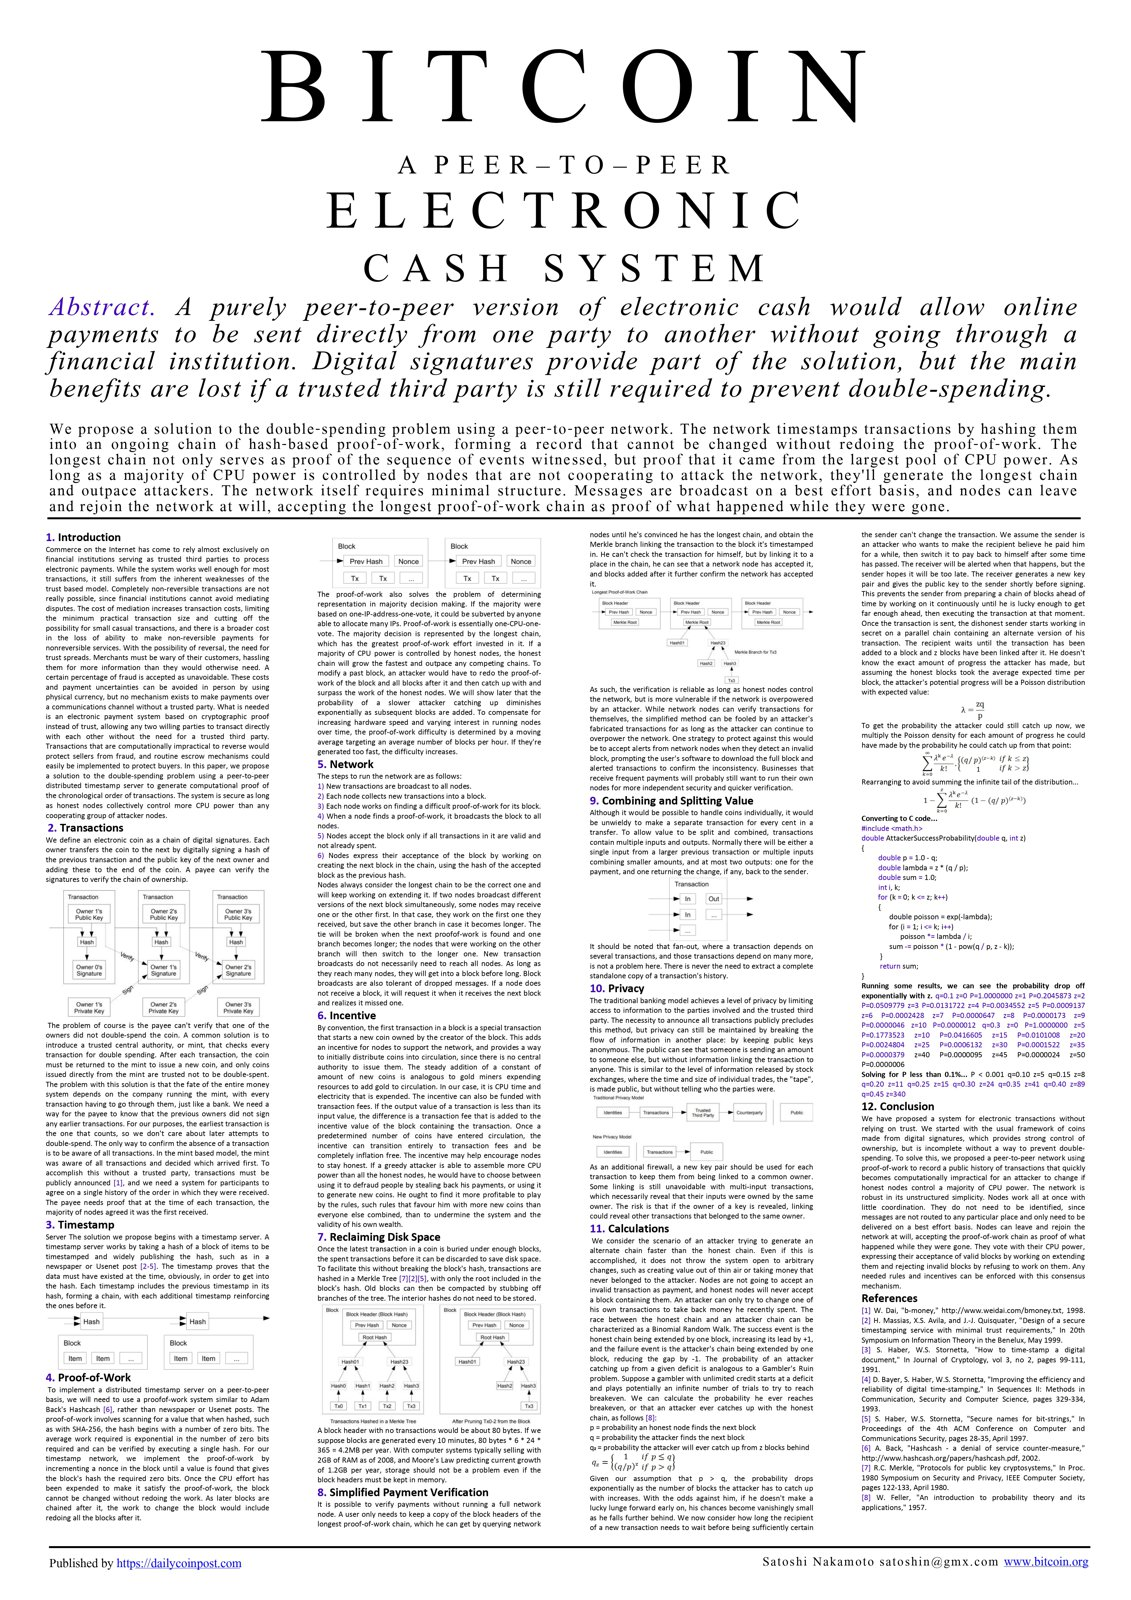
\includegraphics[height=0.50\textheight]{ch0_bitcoin_whitepaper.jpg}\\[1mm]
\imgcap{The Bitcoin white paper, 2008}
\imgcredit{https://commons.wikimedia.org/wiki/File:Bitcoin-whitepaper-poster_page-0001.jpg}{Text: Satoshi Nakamoto (2008); poster: DailyCoinPost (2018); CC0; Wikimedia Commons}
\end{column}
\end{columns}
\end{frame}

\begin{frame}{The Blockchain: a Public Ledger}
\itemsize{\small}
\begin{itemize}
    \item \textbf{Ledger}: the list of all transactions; whoever holds the ledger knows who owns what
    \begin{itemize}
        \item banks keep private ledgers; Bitcoin keeps one public ledger, copied on thousands of computers (\textbf{nodes})
    \end{itemize}
    \item \textbf{Block}: a batch of transactions; \textbf{hash}: a short fingerprint of a block (the function SHA-256)
    \begin{itemize}
        \item changing one character of a block changes its hash completely
        \item each block contains the hash of the previous one: the blocks form a \textbf{chain}
    \end{itemize}
    \item Consequence: rewriting an old transaction means rewriting every later block
    \begin{itemize}
        \item who may add the next block, and at what cost, is decided by the \textbf{consensus} rule (next slide)
    \end{itemize}
    \item Ownership: a coin belongs to whoever holds the private key of its address; a lost key is a lost coin
\end{itemize}
\end{frame}

\begin{frame}{Proof of Work and Mining}
\itemsize{\footnotesize}
\begin{columns}[T]
\begin{column}{0.58\textwidth}
\begin{itemize}
    \item \textbf{Proof of work} (PoW): to add a block, a \textbf{miner} must find a number that makes the hash of the block smaller than a target
    \begin{itemize}
        \item the only method is trial and error: billions of hashes per second, on specialised machines
        \item the target is adjusted every 2016 blocks so that a block arrives about every 10 minutes
    \end{itemize}
    \item The winner receives the \textbf{block subsidy} (new coins) plus the fees of the transactions
    \begin{itemize}
        \item to rewrite history, an attacker would need more computing power than all honest miners together
    \end{itemize}
    \item The cost of security is electricity: this is why Bitcoin is criticised for its energy use
\end{itemize}
\end{column}
\begin{column}{0.39\textwidth}
\centering
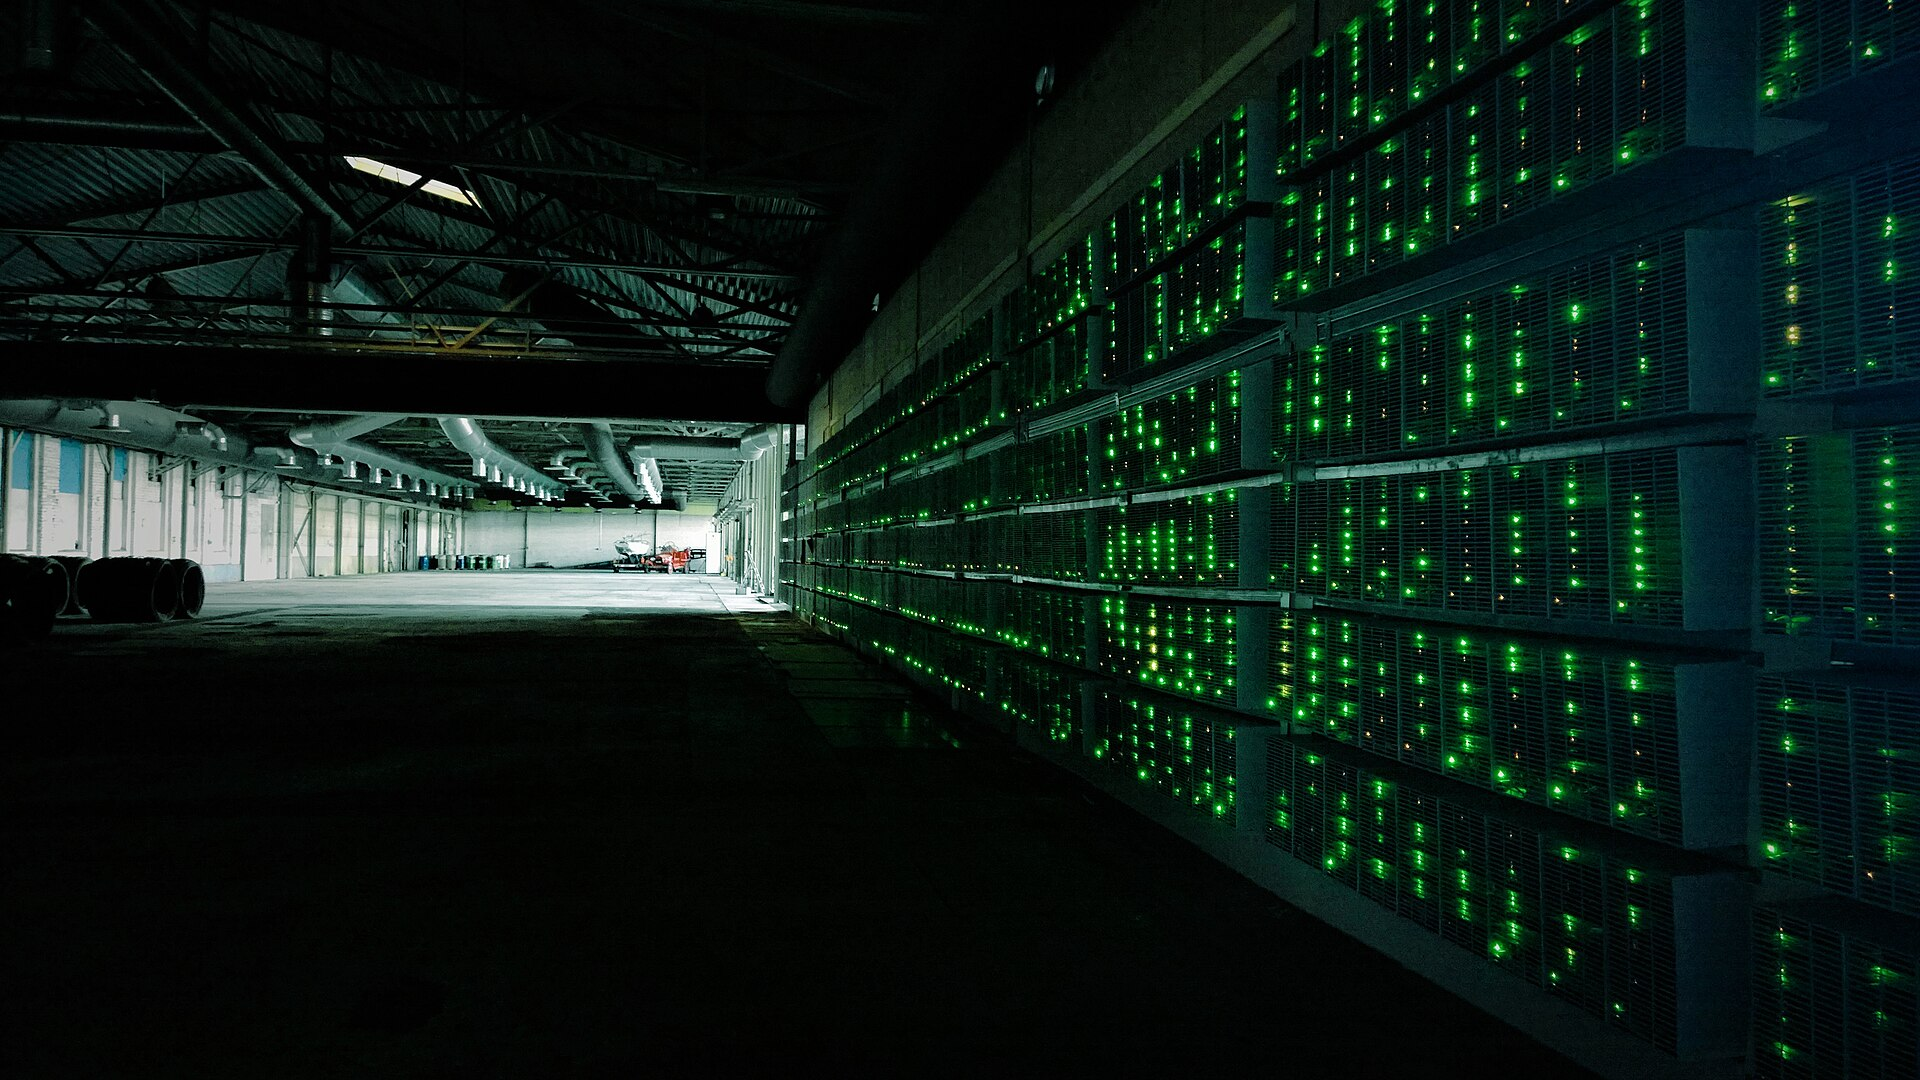
\includegraphics[height=0.36\textheight]{ch14_mining_farm_2014.jpg}\\[1mm]
\imgcap{A Bitcoin mining farm, 2014}
\imgcredit{https://commons.wikimedia.org/wiki/File:Bitcoin_mining_farm.jpg}{Photo: Marko Ahtisaari (2014); CC BY 2.0; Wikimedia Commons}
\end{column}
\end{columns}
\end{frame}

\begin{frame}{The Supply Rule and the Halving}
\itemsize{\small}
\begin{itemize}
    \item Block subsidy: 50 BTC from 2009, \textbf{halved} every 210\,000 blocks (about four years)
    \begin{itemize}
        \item 2012: 25; 2016: 12.5; 2020: 6.25; April 2024: 3.125 BTC per block
        \item the event of halving the subsidy is called the \textbf{halving}
    \end{itemize}
    \item Total supply: a geometric series
    \begin{itemize}
        \item $210\,000 \times 50 \times (1 + \tfrac12 + \tfrac14 + \dots) = 210\,000 \times 50 \times 2 = 21$ million BTC
        \item about 19.4 million at the start of 2024, 20.4 million in 2030: almost all coins already exist
    \end{itemize}
    \item The halving dates are known years in advance
    \begin{itemize}
        \item in an efficient market (\sfmchlink{https://danpele.github.io/SFM/EN/Courses/chapter7_efficient_markets_random_walk_vr.pdf}{Chapter 7}), a predictable cut in new supply should already be in the price
    \end{itemize}
\end{itemize}
\end{frame}

\begin{frame}{Bitcoin Price and Supply}
\itemsize{\footnotesize}
\begin{center}
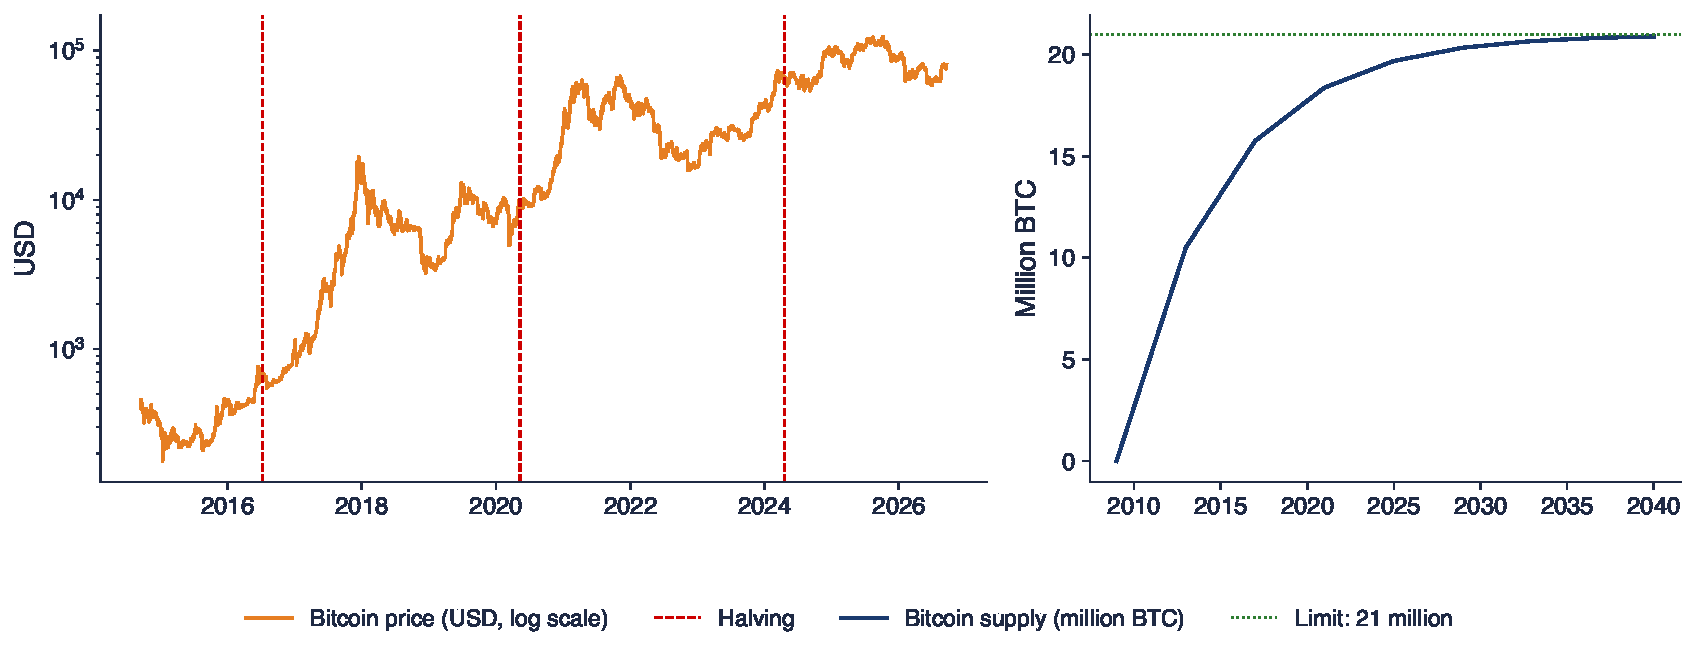
\includegraphics[width=0.97\textwidth,height=0.50\textheight,keepaspectratio]{sfm_ch14_halving.pdf}
\end{center}
\vspace{-0.25cm}
\begin{itemize}
    \item Left: Bitcoin close in USD (log scale), 457 USD in September 2014 and 80\,901 USD on 18 September 2026; dashed: the halvings of 2016, 2020 and 2024. Right: supply from the protocol rule
    \item Interpretation: one year after the halvings the price was 287\%, 559\% and 31\% higher; three observations are not evidence, and the effect shrinks
\end{itemize}
\sfmquantlet{Ch_14}{SFM_ch14_bitcoin_basics}
\end{frame}

\begin{frame}{An Anonymous Founder}
\itemsize{\footnotesize}
\begin{columns}[T]
\begin{column}{0.62\textwidth}
\begin{itemize}
    \item Nobody knows who ``Satoshi Nakamoto'' is; the founder stopped writing in 2011
    \begin{itemize}
        \item the rules of Bitcoin are changed only if most nodes accept the new software
    \end{itemize}
    \item Consequences for a statistician
    \begin{itemize}
        \item no company, no profits, no dividends: no cash flows to discount
        \item the price reflects only demand: payments, speculation, belief in scarcity \refBHL
        \item so the usual valuation models do not apply; we study the price as a statistical object
    \end{itemize}
    \item Trades happen around the clock on hundreds of exchanges, 365 days a year
\end{itemize}
\end{column}
\begin{column}{0.35\textwidth}
\centering
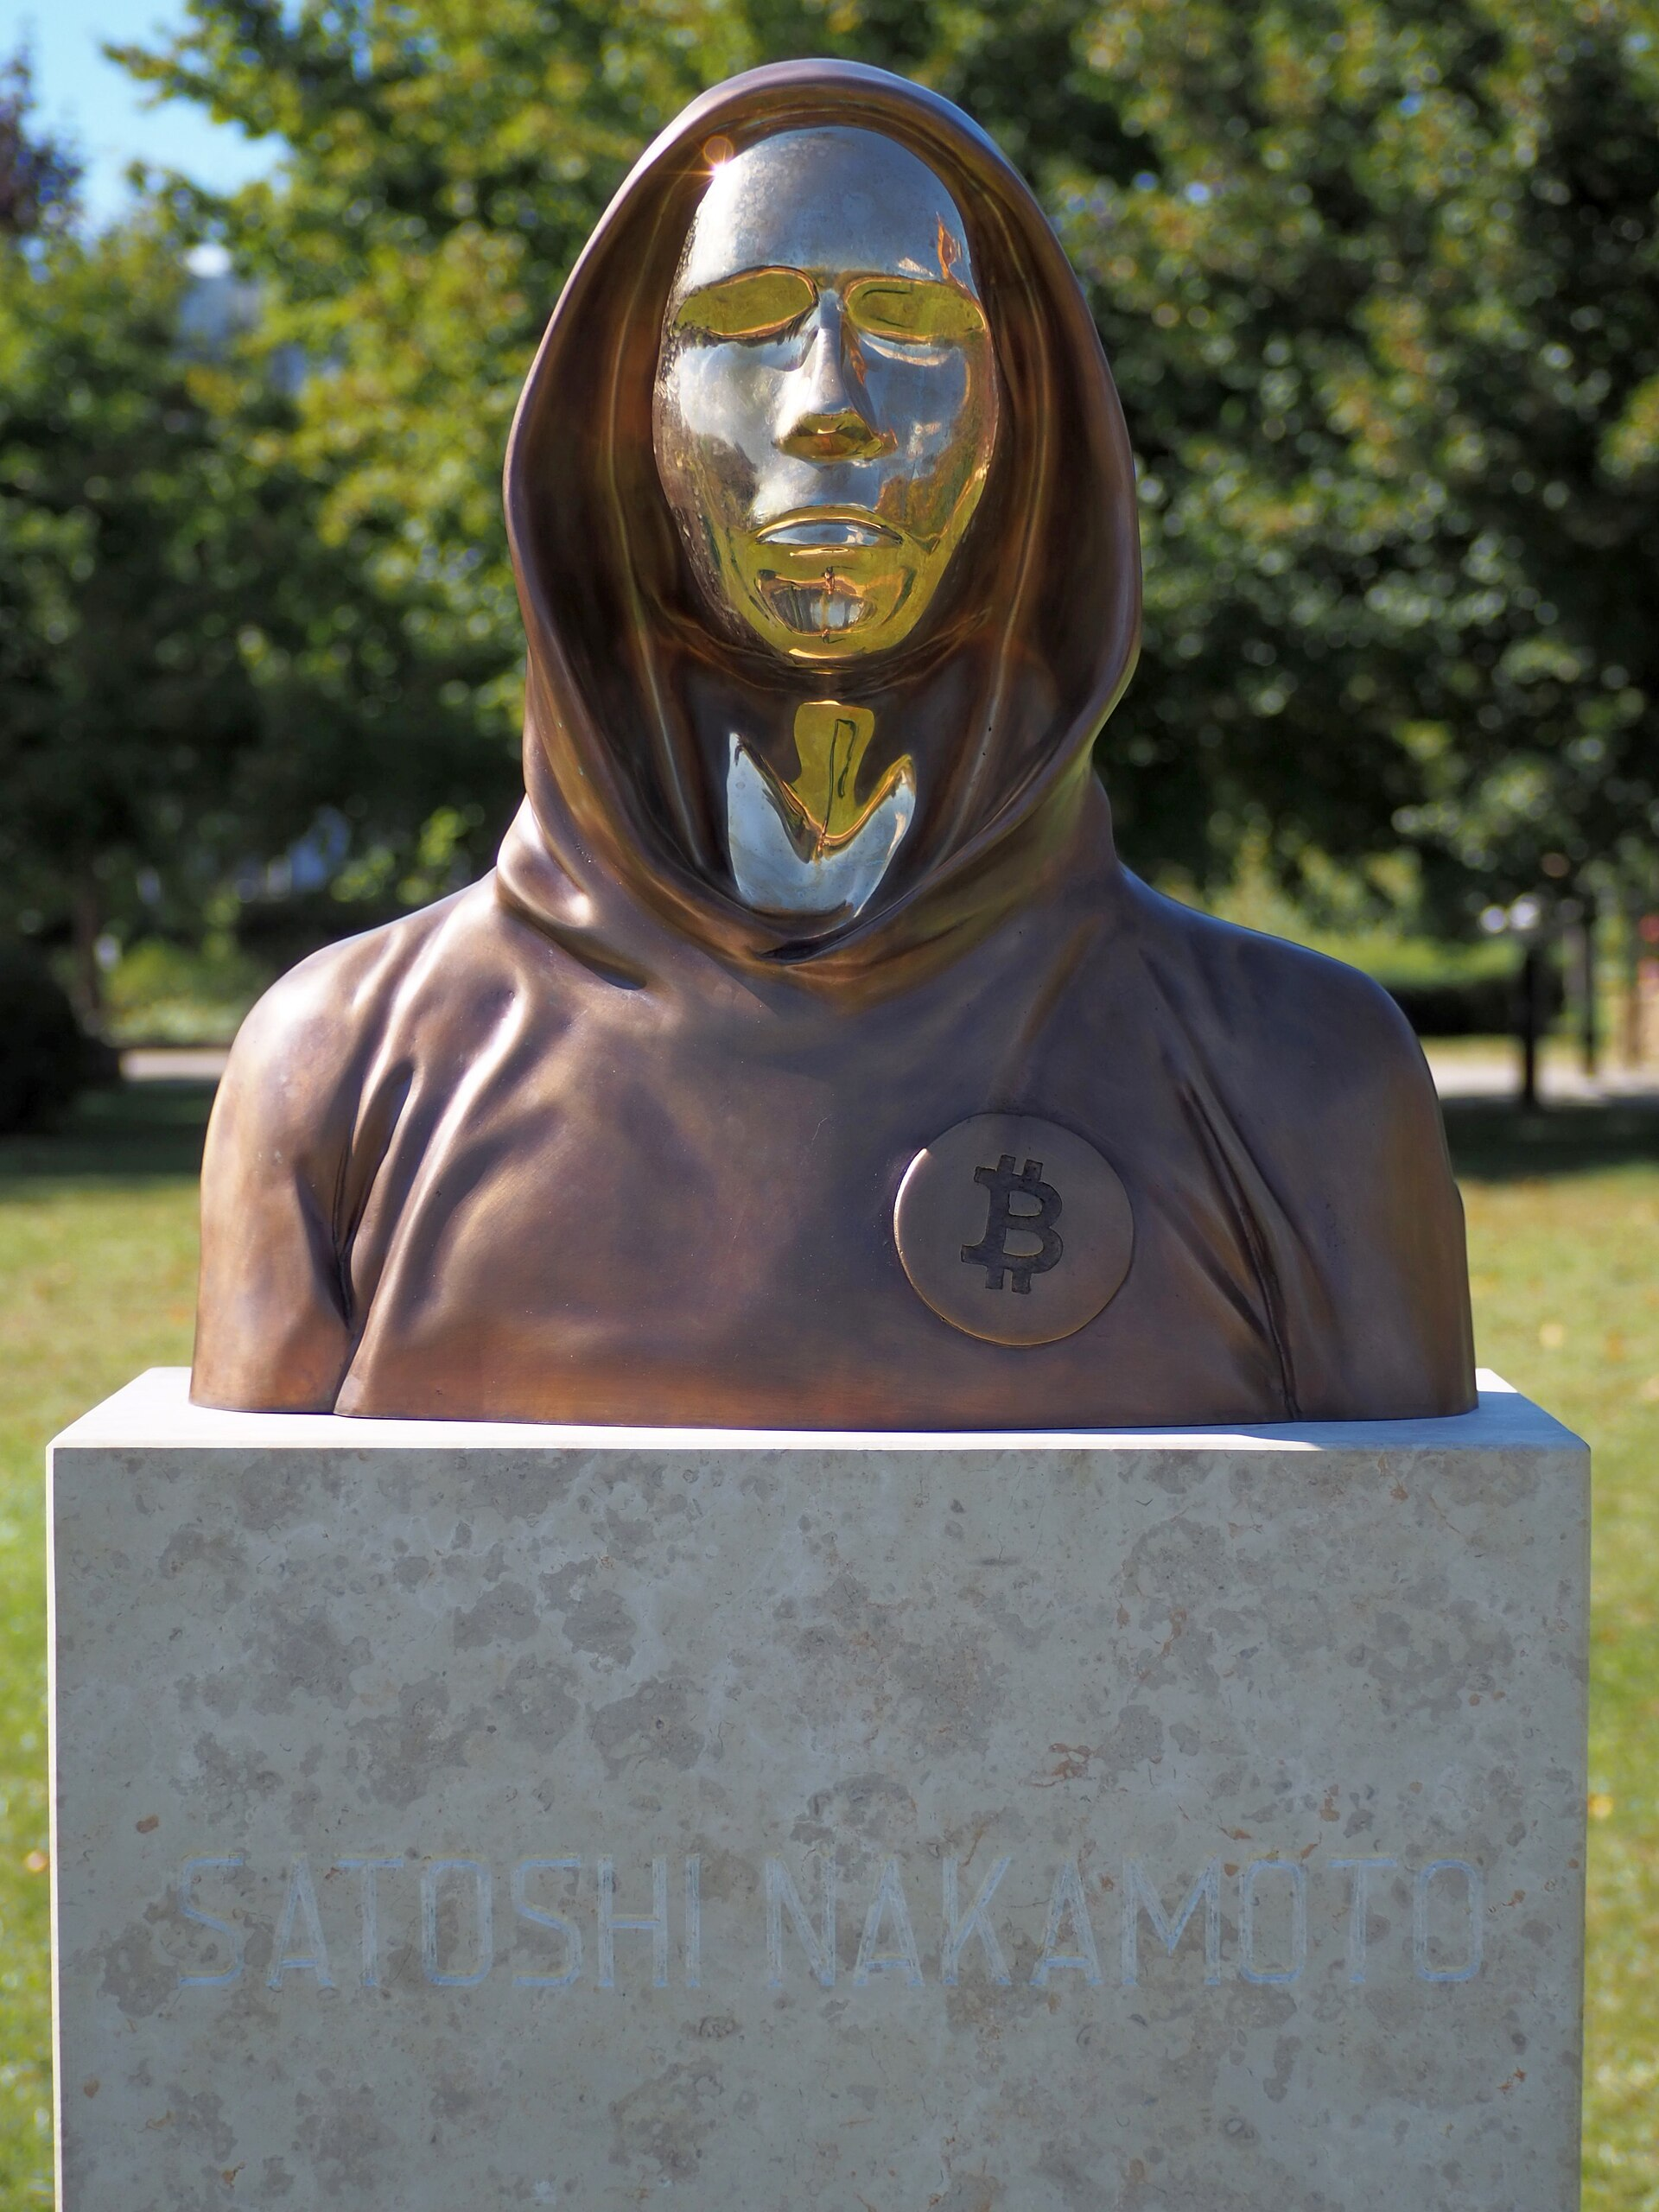
\includegraphics[height=0.46\textheight]{ch14_satoshi_bust_2021.jpg}\\[1mm]
\imgcap{A bust of Satoshi Nakamoto, Budapest}
\imgcredit{https://commons.wikimedia.org/wiki/File:Bust_of_Satoshi_Nakamoto_in_Budapest.jpg}{Photo: Fekist (2021); CC BY-SA 4.0; Wikimedia Commons}
\end{column}
\end{columns}
\end{frame}

\begin{frame}{Ethereum, Smart Contracts and Proof of Stake}
\itemsize{\footnotesize}
\begin{columns}[T]
\begin{column}{0.64\textwidth}
\begin{itemize}
    \item 2014: \refButerin{} proposes Ethereum, a blockchain that runs programs; launched in July 2015
    \begin{itemize}
        \item \textbf{smart contract}: a program stored on the blockchain that executes a transaction when its conditions are met
        \item on top of it: tokens, stablecoins and DeFi (decentralised finance: lending and trading without intermediaries)
    \end{itemize}
    \item \textbf{Proof of stake} (PoS): the right to add a block is drawn in proportion to the coins locked as a deposit (\textbf{stake})
    \begin{itemize}
        \item cheating is punished by losing the stake; no race of computing power
        \item 15 September 2022 (``the Merge''): Ethereum moves from PoW to PoS; energy use falls by more than 99.9\% \refMerge
    \end{itemize}
\end{itemize}
\end{column}
\begin{column}{0.33\textwidth}
\centering
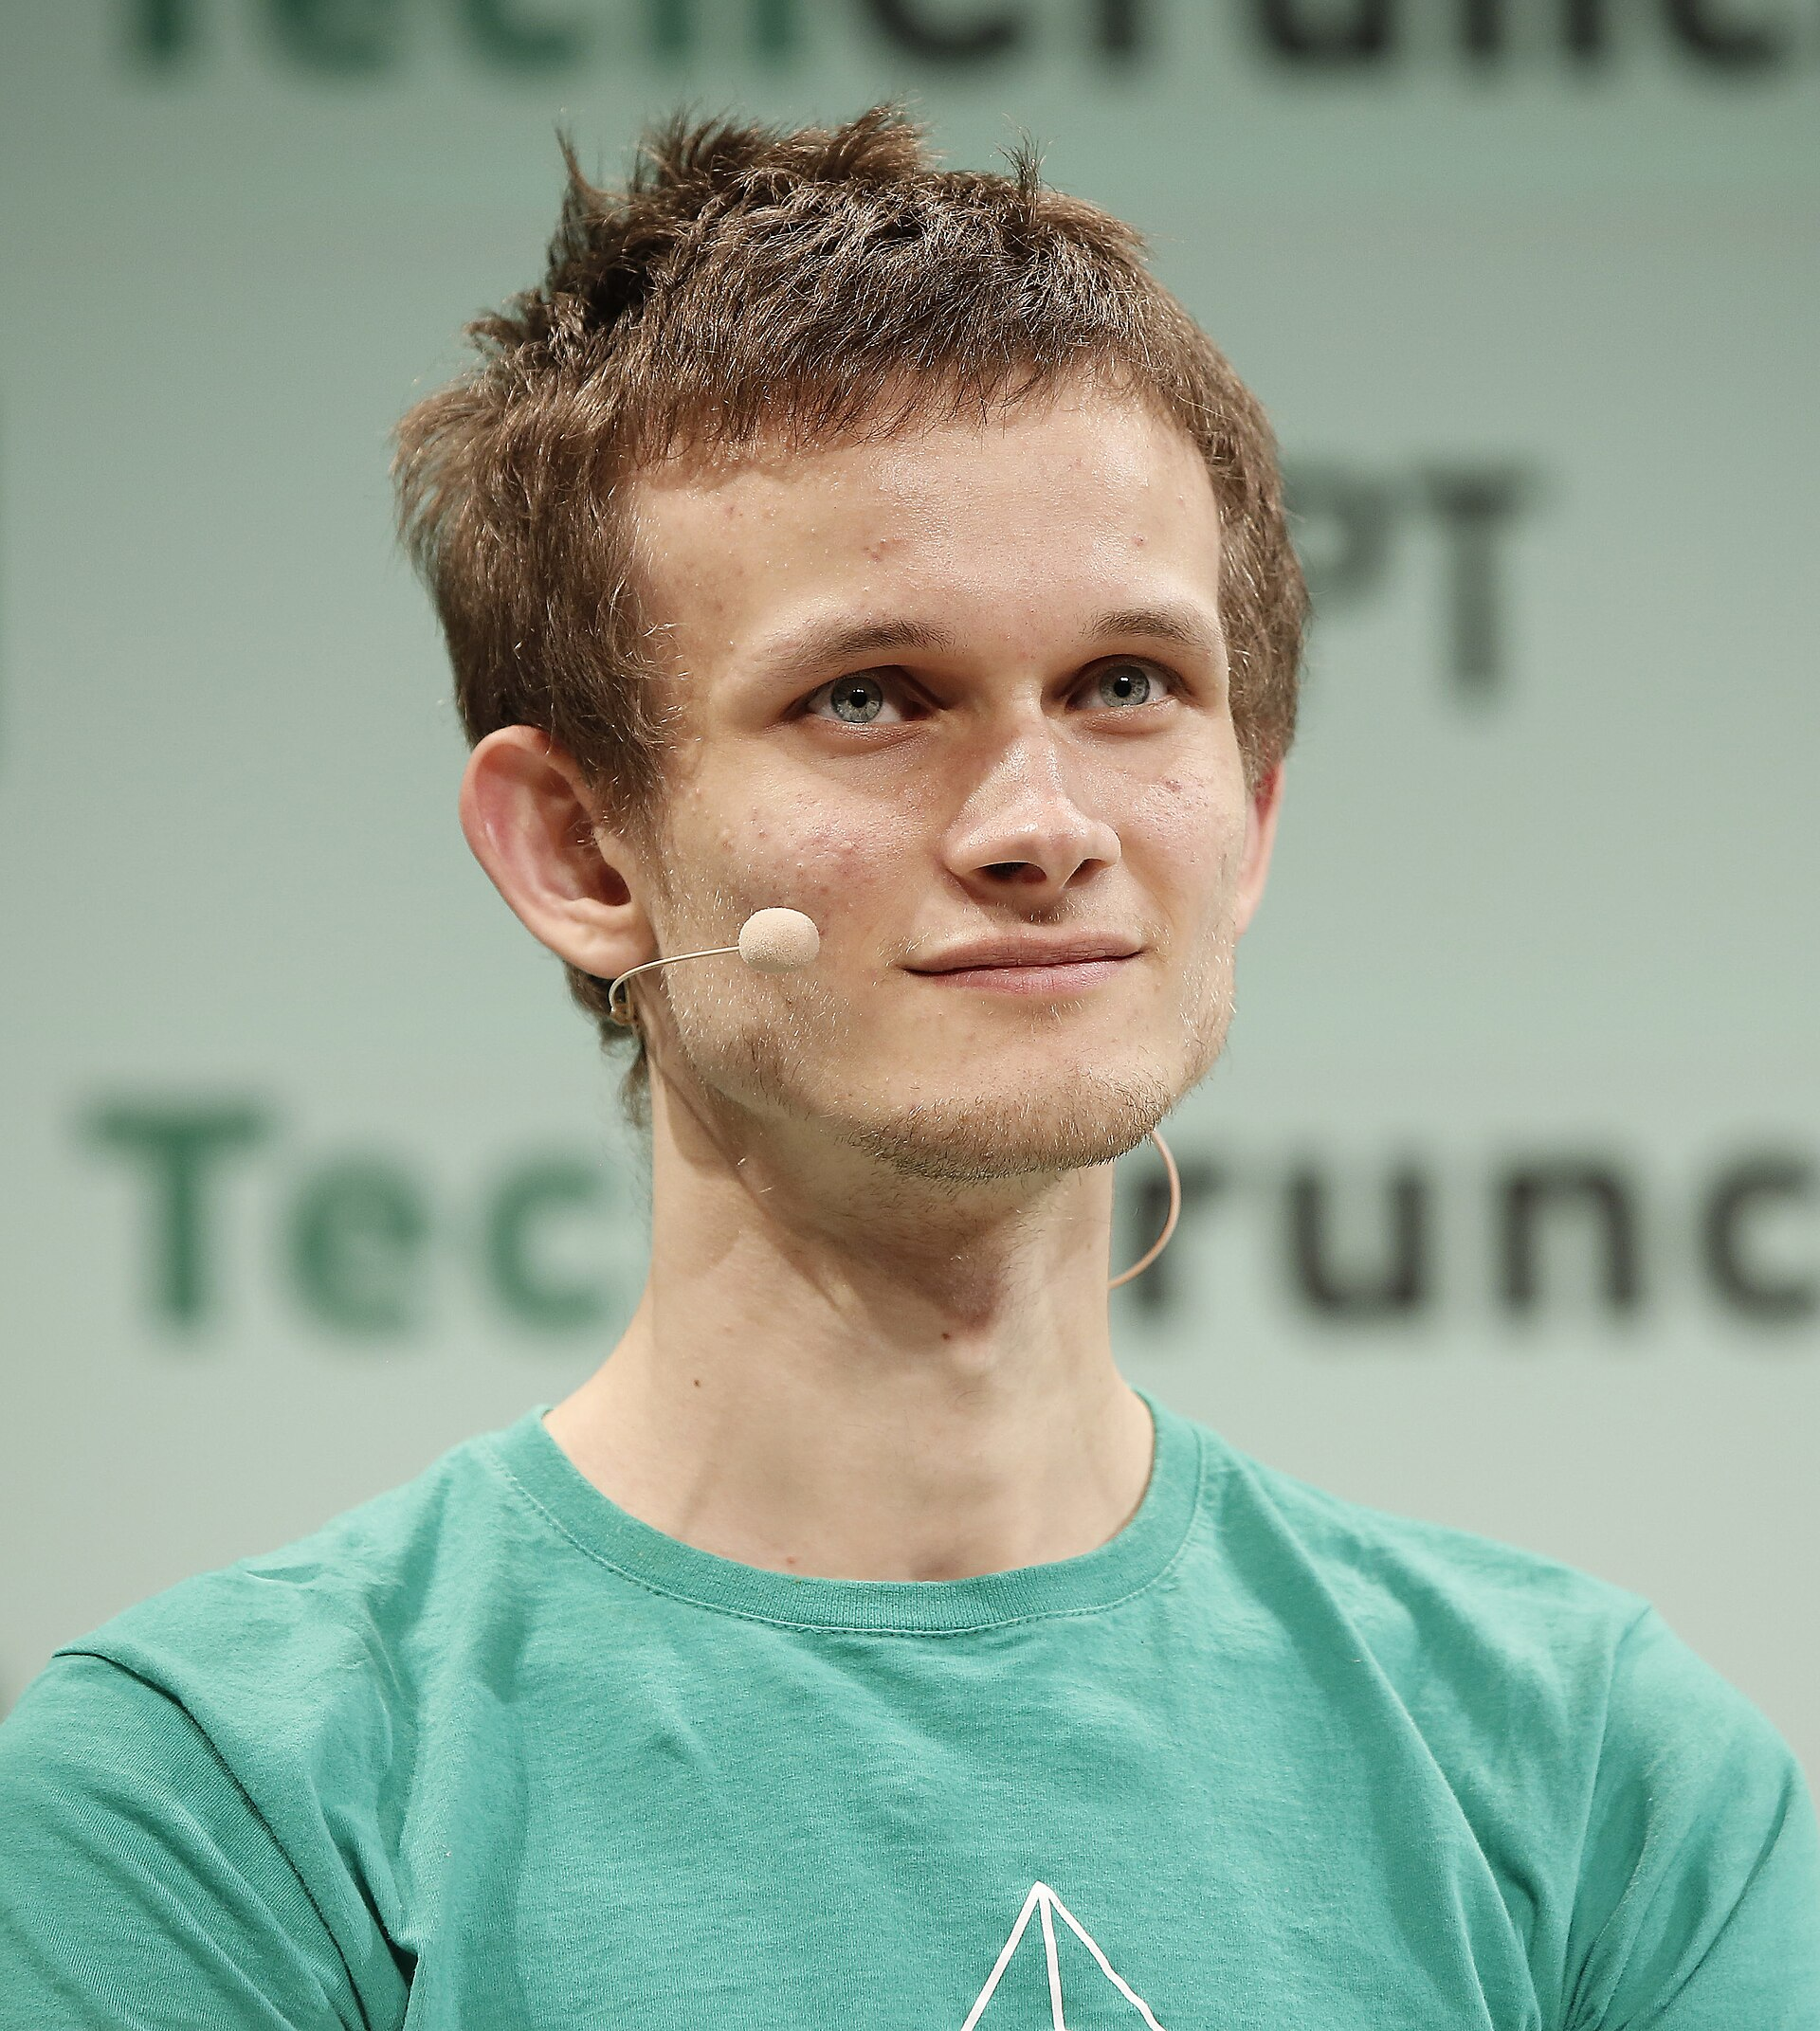
\includegraphics[height=0.42\textheight]{ch14_buterin_2015.jpg}\\[1mm]
\imgcap{Vitalik Buterin, 2015}
\imgcredit{https://commons.wikimedia.org/wiki/File:Vitalik_Buterin_TechCrunch_London_2015_(cropped).jpg}{Photo: John Phillips (2015); CC BY 2.0; Wikimedia Commons}
\end{column}
\end{columns}
\end{frame}

\begin{frame}{Prices and Data}
\itemsize{\footnotesize}
\begin{columns}[T]
\begin{column}{0.64\textwidth}
\begin{itemize}
    \item There is no single exchange: each platform has its own price; prices differ across countries \refMS
    \begin{itemize}
        \item a data provider aggregates the platforms into one daily series; here: EODHD, close at midnight UTC (Coordinated Universal Time)
    \end{itemize}
    \item Seven trading days a week: no weekend gaps, no holidays
    \begin{itemize}
        \item Bitcoin: 4\,384 daily returns since 2014; the S\&P 500: 3\,017 returns in the same period
    \end{itemize}
    \item Market indices of many coins exist, e.g.\ CRIX (Crypto Index) \refTH
    \begin{itemize}
        \item CRIX chooses the number of coins with the AIC criterion (\sfmchlink{https://danpele.github.io/SFM/EN/Courses/chapter6_model_selection_risk_management.pdf}{Chapter 6}): few coins describe the whole market
    \end{itemize}
    \item Returns: $r_t = 100(\ln P_t - \ln P_{t-1})$ in \%, each series on its own calendar
\end{itemize}
\end{column}
\begin{column}{0.33\textwidth}
\centering
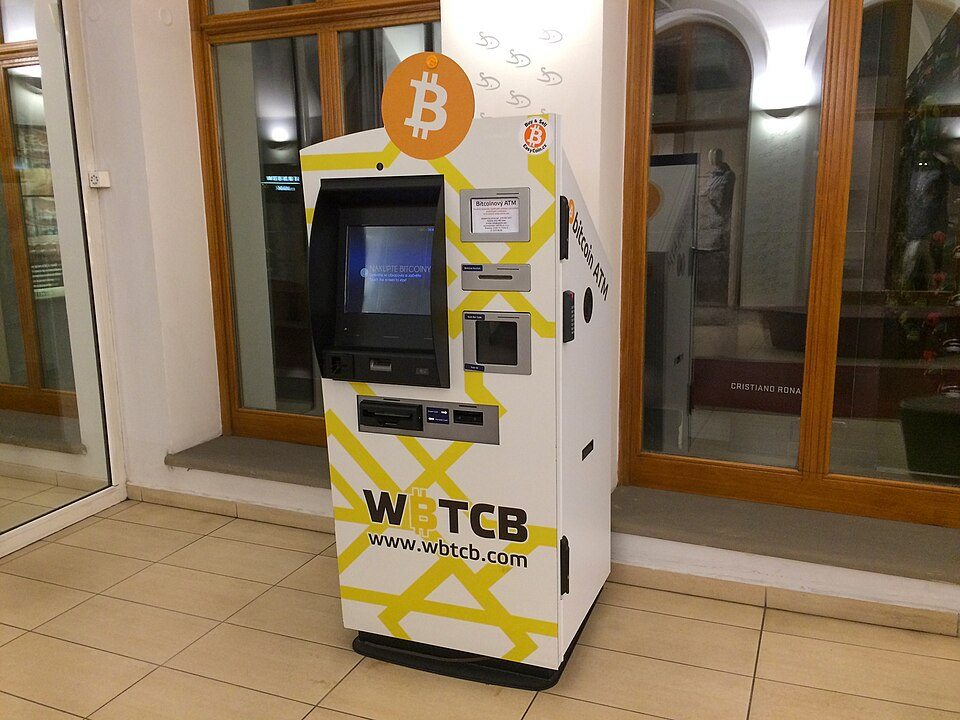
\includegraphics[height=0.40\textheight]{ch11_bitcoin_atm_prague.jpg}\\[1mm]
\imgcap{A Bitcoin ATM, Prague}
\imgcredit{https://commons.wikimedia.org/wiki/File:Bitcoin_ATM_Prague.jpg}{Photo: Perituss (2016); CC0; Wikimedia Commons}
\end{column}
\end{columns}
\end{frame}

\begin{frame}{Recap: Bitcoin and Ethereum in Brief}
\itemsize{\small}
\begin{itemize}
    \item A blockchain is a public chain of blocks linked by hashes; changing the past means redoing all later work
    \item PoW pays miners for computing; PoS asks validators for a deposit; Ethereum switched in 2022
    \item The Bitcoin supply is fixed by the halving rule at 21 million; there are no cash flows, only prices
\end{itemize}
\end{frame}


%=============================================================================
\section{Crypto as an Asset Class}
%=============================================================================

\begin{frame}{Annualisation with the Actual Frequency}
\itemsize{\footnotesize}
\begin{itemize}
    \item With $m$ observations a year and i.i.d.\ daily returns: annual mean $= m\,\bar r$, annual volatility $= \sqrt{m}\,s$ (\sfmchlink{https://danpele.github.io/SFM/EN/Courses/chapter1_data_returns_indicators.pdf}{Chapter 1})
    \begin{itemize}
        \item equities: $m \approx 252$ trading days; crypto: $m = 365$ (actual frequency: $m = 365.3$ for Bitcoin, 251.4 for the S\&P 500)
    \end{itemize}
    \item \textbf{Worked example}: Bitcoin, $\bar r = 0.118\%$, $s = 3.49\%$ per day
    \begin{itemize}
        \item right: $\sqrt{365} \times 3.49 = 19.10 \times 3.49 = 66.6\%$; mean $365 \times 0.118 = 43.1\%$
        \item wrong: $\sqrt{252} \times 3.49 = 55.3\%$ and $252 \times 0.118 = 29.8\%$
    \end{itemize}
    \item The 252 rule understates the volatility by 16.9\% and the mean by 31.0\%
    \begin{itemize}
        \item mixing the two (mean $\times 252$, volatility $\times\sqrt{365}$) also biases the Sharpe ratio
        \item comparisons with equities: annualise each series with its own $m$, never with a common one
    \end{itemize}
\end{itemize}
\end{frame}

\begin{frame}{Five Assets Side by Side}
\itemsize{\footnotesize}
\begin{center}
\scriptsize
\begin{tabular}{lrrrrrrrr}
\toprule
& since & $n$ & mean (\%) & sd (\%) & ann.\ vol.\ (\%) & skew. & exc.\ kurt. & min (\%) \\
\midrule
Bitcoin & 2014 & 4\,384 & $0.118$ & $3.49$ & $66.6$ & $-0.70$ & $12.0$ & $-46.5$ \\
Ethereum & 2016 & 3\,913 & $0.202$ & $4.99$ & $95.3$ & $-0.20$ & $9.0$ & $-55.1$ \\
Solana & 2020 & 2\,351 & $0.212$ & $6.12$ & $117.1$ & $-0.22$ & $7.9$ & $-55.0$ \\
S\&P 500 & 2014 & 3\,017 & $0.044$ & $1.11$ & $17.6$ & $-0.64$ & $15.8$ & $-12.8$ \\
Gold & 2014 & 3\,124 & $0.041$ & $1.01$ & $16.4$ & $-0.41$ & $9.5$ & $-11.1$ \\
\bottomrule
\end{tabular}
\end{center}
\begin{itemize}
    \item Daily log returns until 18 September 2026; annual volatility $= \sqrt{m}\,s$ with the actual frequency $m$ of each series; gold: XAU/USD
    \item Interpretation
    \begin{itemize}
        \item Bitcoin is 3.8 times as volatile as the S\&P 500 (66.6\% against 17.6\%); Ethereum 5.4 times, Solana 6.7 times
        \item on 11.6\% of the days Bitcoin moves by more than 5\%; the worst day: $-46.5\%$ on 12 March 2020
        \item all five have negative skewness and excess kurtosis: the stylised facts of \sfmchlink{https://danpele.github.io/SFM/EN/Courses/chapter2_classical_distributions_stylised_facts.pdf}{Chapter 2} hold, in a stronger form
    \end{itemize}
\end{itemize}
\end{frame}

\begin{frame}{Volatility Through Time}
\itemsize{\footnotesize}
\begin{center}
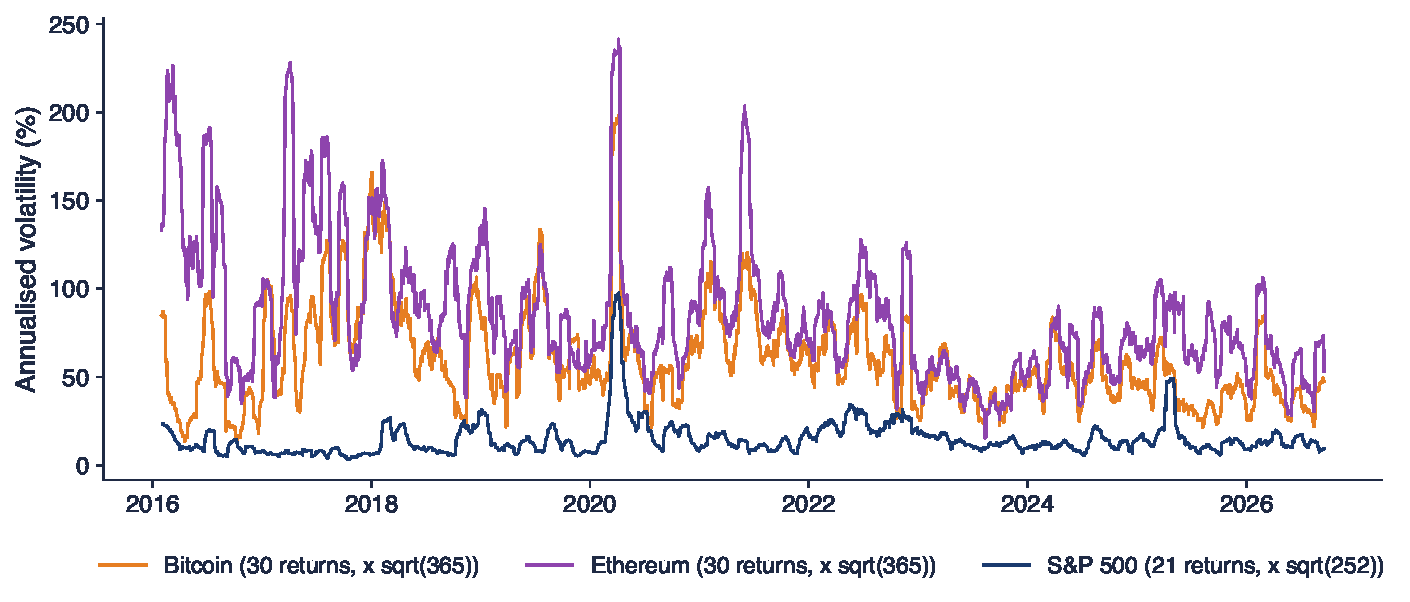
\includegraphics[width=0.97\textwidth,height=0.46\textheight,keepaspectratio]{sfm_ch14_rolling_vol.pdf}
\end{center}
\vspace{-0.25cm}
\begin{itemize}
    \item Volatility on about one month: 30 daily returns $\times\sqrt{365}$ for crypto, 21 returns $\times\sqrt{252}$ for the S\&P 500
    \item Interpretation: medians 54\% (Bitcoin), 77\% (Ethereum), 12\% (S\&P 500); the median ratio Bitcoin/S\&P 500 is 3.8; all three peak in March--April 2020
    \item Bitcoin's volatility trends down, but it was below that of the S\&P 500 on only 0.1\% of the days
\end{itemize}
\sfmquantlet{Ch_14}{SFM_ch14_asset_class}
\end{frame}

\begin{frame}{Case Study: Risks and Returns of Cryptocurrency}
\itemsize{\small}
\begin{itemize}
    \item \refLT: Bitcoin, Ripple and Ethereum, daily and weekly returns, 2011--2018
    \begin{itemize}
        \item design: regress crypto returns on stock-market factors, currencies, commodities and macroeconomic factors
    \end{itemize}
    \item Findings
    \begin{itemize}
        \item crypto returns have almost no exposure to the usual factors: a separate asset class
        \item strong time-series momentum: high returns this week predict high returns in the next weeks
        \item investor attention (Google searches, Twitter posts) predicts returns
    \end{itemize}
    \item Follow-up \refLTW: three crypto factors (market, size, momentum) price the cross-section of coins
    \begin{itemize}
        \item the link with equities has changed since 2020 (Section 5): results depend on the sample period
    \end{itemize}
\end{itemize}
\end{frame}

\begin{frame}{Is the Weekend Different?}
\itemsize{\small}
\begin{itemize}
    \item Stock markets close at weekends; crypto markets do not, but banks, institutional traders and news slow down
    \begin{itemize}
        \item \textbf{weekday effect}: different mean or variance of returns on some days of the week \refCP
    \end{itemize}
    \item Two tests on Bitcoin, each day labelled by its closing date
    \begin{itemize}
        \item mean: $r_t = a + b\,W_t + \varepsilon_t$, $W_t = 1$ on Saturday and Sunday; HAC (Newey--West) standard errors
        \item variance: the Brown--Forsythe test (Levene's test around the median), robust to heavy tails
    \end{itemize}
    \item Ratio of the weekend to the weekday variance: equal to 1 if every day had the same risk
\end{itemize}
\end{frame}

\begin{frame}{Bitcoin Volatility by Day of the Week}
\itemsize{\footnotesize}
\begin{center}
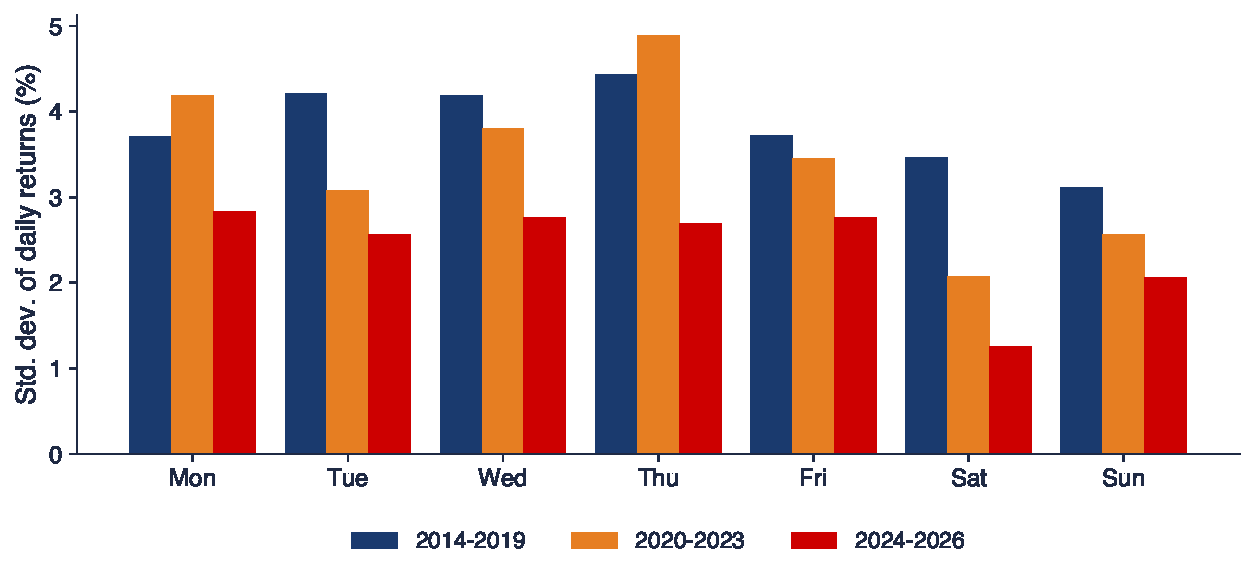
\includegraphics[width=0.97\textwidth,height=0.44\textheight,keepaspectratio]{sfm_ch14_weekday.pdf}
\end{center}
\vspace{-0.25cm}
\begin{itemize}
    \item Standard deviation of daily returns by closing day; three periods
    \item Weekend dummy $b$ (p-value): $-0.01$ (0.95), $-0.11$ (0.48), $-0.03$ (0.83): no weekend effect in the mean
    \item Interpretation: weekend/weekday variance 0.66, 0.35, 0.39 (Brown--Forsythe p 0.002, $<$\,0.001, $<$\,0.001): crypto is calmer when traditional markets close
\end{itemize}
\sfmquantlet{Ch_14}{SFM_ch14_asset_class}
\end{frame}

\begin{frame}{Recap: Crypto as an Asset Class}
\itemsize{\small}
\begin{itemize}
    \item Annualise crypto with 365 days: Bitcoin 66.6\% a year, not 55.3\%
    \item Crypto volatility is 3.8 (Bitcoin) to 6.7 (Solana) times that of the S\&P 500, and decreasing
    \item No weekend effect in the mean, a strong one in the variance
\end{itemize}
\end{frame}


%=============================================================================
\section{Tails and Volatility Clustering}
%=============================================================================

\begin{frame}{Heavy Tails: the Hill Estimator}
\itemsize{\footnotesize}
\begin{center}
\scriptsize
\begin{tabular}{lrrrr}
\toprule
& left tail $\hat\alpha$ & 95\% CI & right tail $\hat\alpha$ & 95\% CI \\
\midrule
Bitcoin & $2.71$ & $[2.20, 3.21]$ & $3.37$ & $[2.74, 4.00]$ \\
Ethereum & $2.62$ & $[2.10, 3.15]$ & $3.09$ & $[2.48, 3.71]$ \\
Solana & $2.84$ & $[2.11, 3.57]$ & $3.41$ & $[2.54, 4.29]$ \\
S\&P 500 & $2.68$ & $[2.08, 3.29]$ & $2.80$ & $[2.17, 3.43]$ \\
Gold & $3.11$ & $[2.42, 3.80]$ & $3.04$ & $[2.36, 3.71]$ \\
\bottomrule
\end{tabular}
\end{center}
\begin{itemize}
    \item \refHill{} (\sfmchlink{https://danpele.github.io/SFM/EN/Courses/chapter5_heavy_tails_evt.pdf}{Chapter 5}): $\hat\alpha = \big[\frac1k\sum_{i=1}^k \ln(X_{(i)}/X_{(k+1)})\big]^{-1}$ on the $k$ largest losses (or gains), $k = 2.5\%$ of $n$; CI: $\hat\alpha(1 \pm 1.96/\sqrt{k})$
    \begin{itemize}
        \item $P(X > x) \approx c\,x^{-\alpha}$: moments of order $\ge \alpha$ are infinite
    \end{itemize}
    \item Interpretation: Bitcoin's left tail ($\hat\alpha = 2.71$) is heavier than its right tail; with $\alpha < 4$ the kurtosis is not finite, so the sample kurtosis is not a stable number; the intervals of crypto and equities overlap
\end{itemize}
\end{frame}

\begin{frame}{Volatility Clustering in Bitcoin}
\itemsize{\footnotesize}
\begin{center}
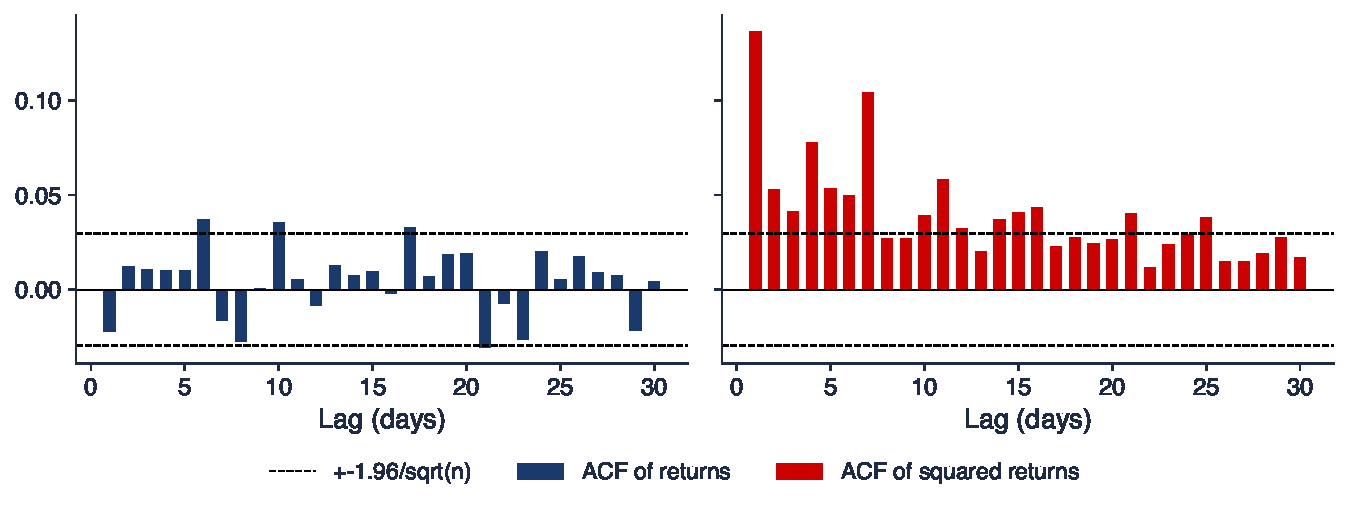
\includegraphics[width=0.97\textwidth,height=0.46\textheight,keepaspectratio]{sfm_ch14_acf.pdf}
\end{center}
\vspace{-0.25cm}
\begin{itemize}
    \item ACF (autocorrelation function) of $r_t$ and of $r_t^2$, lags 1--30; dashed: $\pm 1.96/\sqrt{n} = \pm 0.030$
    \item Returns: $\hat\rho(1) = -0.022$, 4 of 30 lags outside the band; squared returns: $\hat\rho(1) = 0.137$, 15 of 30 outside
    \item Interpretation: Ljung--Box $Q(10)$ is 20.2 for $r_t$ and 212.7 for $r_t^2$ (p $<$\,0.001): the direction is hard to predict, the size of the move is not
\end{itemize}
\sfmquantlet{Ch_14}{SFM_ch14_garch_efficiency}
\end{frame}

\begin{frame}{GARCH(1,1)-t for Crypto and Traditional Assets}
\itemsize{\footnotesize}
\begin{center}
\scriptsize
\begin{tabular}{lrrrrrrr}
\toprule
& $\hat\omega$ & $\hat\alpha$ & $\hat\beta$ & $\hat\alpha + \hat\beta$ & half-life (days) & $\hat\nu$ & GJR $\hat\gamma$ ($t$) \\
\midrule
Bitcoin & $0.194$ & $0.109$ & $0.891$ & $1.000$ & -- & $3.18$ & $-0.013$ ($-0.72$) \\
Ethereum & $1.067$ & $0.175$ & $0.825$ & $1.000$ & -- & $3.14$ & $0.032$ ($0.91$) \\
S\&P 500 & $0.024$ & $0.173$ & $0.820$ & $0.993$ & 100 & $5.50$ & $0.280$ ($7.08$) \\
Gold & $0.010$ & $0.047$ & $0.947$ & $0.994$ & 113 & $4.13$ & $-0.051$ ($-3.33$) \\
\bottomrule
\end{tabular}
\end{center}
\begin{itemize}
    \item \refBoll{} (\sfmchlink{https://danpele.github.io/SFM/EN/Courses/chapter9_arch_garch_models.pdf}{Chapter 9}): $\sigma_t^2 = \omega + \alpha\varepsilon_{t-1}^2 + \beta\sigma_{t-1}^2$, Student-t innovations with $\nu$ degrees of freedom; half-life of a shock $\ln 0.5/\ln(\alpha + \beta)$
    \begin{itemize}
        \item GJR: an extra term $\gamma\,\varepsilon_{t-1}^2\mathbb{1}\{\varepsilon_{t-1} < 0\}$; $\gamma > 0$ is the leverage effect of equities
    \end{itemize}
\end{itemize}
\end{frame}

\begin{frame}{Interpretation of the GARCH Estimates}
\itemsize{\small}
\begin{itemize}
    \item Crypto: $\hat\alpha + \hat\beta = 1$ at the boundary: an integrated GARCH (IGARCH; the EWMA of \sfmchlink{https://danpele.github.io/SFM/EN/Courses/chapter8_volatility_estimators.pdf}{Chapter 8} is the case $\omega = 0$)
    \begin{itemize}
        \item a shock to volatility does not die out within the sample; there is no finite long-run variance to which volatility returns
        \item S\&P 500 and gold: half-lives of 100 and 113 days
    \end{itemize}
    \item $\hat\nu \approx 3.18$ for Bitcoin: even after GARCH filtering the tails are very heavy
    \begin{itemize}
        \item the S\&P 500 has $\hat\nu = 5.50$
    \end{itemize}
    \item No leverage effect in crypto: $\hat\gamma = -0.013$ ($t = -0.72$) for Bitcoin, against $0.280$ ($t = 7.08$) for the S\&P 500
    \begin{itemize}
        \item gold has $\hat\gamma < 0$ ($t = -3.33$): rises in its price raise volatility more than falls, as for a safe haven
    \end{itemize}
    \item \refKatsiampa{} compares GARCH-type models for Bitcoin: a model with a short-run and a long-run volatility component fits best
\end{itemize}
\end{frame}

\begin{frame}{Conditional Volatility: Bitcoin and the S\&P 500}
\itemsize{\footnotesize}
\begin{center}
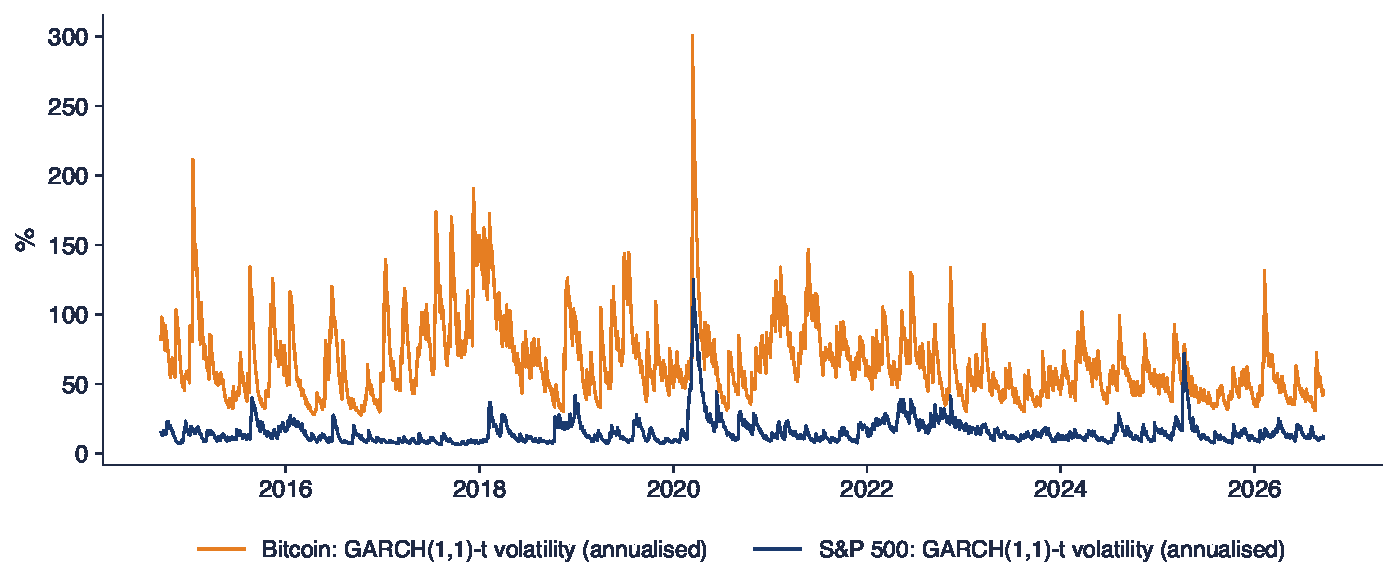
\includegraphics[width=0.97\textwidth,height=0.48\textheight,keepaspectratio]{sfm_ch14_garch_vol.pdf}
\end{center}
\vspace{-0.25cm}
\begin{itemize}
    \item GARCH(1,1)-t volatility $\hat\sigma_t$, annualised with $\sqrt{365}$ (Bitcoin) and $\sqrt{252}$ (S\&P 500)
    \item Interpretation: both peak in March 2020 (301\% and 125\%); on 18 September 2026 the model gives 42\% for Bitcoin and 12\% for the S\&P 500
\end{itemize}
\sfmquantlet{Ch_14}{SFM_ch14_garch_efficiency}
\end{frame}

\begin{frame}{Recap: Tails and Volatility Clustering}
\itemsize{\small}
\begin{itemize}
    \item Crypto tails are heavy ($\hat\alpha$ between 2.5 and 3.5), as heavy in shape as those of the S\&P 500; crypto differs in scale
    \item Volatility clusters strongly; GARCH-t fits with $\alpha + \beta \approx 1$ (IGARCH)
    \item No leverage effect: bad and good news move crypto volatility alike
\end{itemize}
\end{frame}


%=============================================================================
\section{Is the Crypto Market Efficient?}
%=============================================================================

\begin{frame}{Weak-Form Efficiency: What We Test}
\itemsize{\small}
\begin{itemize}
    \item \refFama: in a weak-form efficient market, past prices do not help to predict future returns (\sfmchlink{https://danpele.github.io/SFM/EN/Courses/chapter7_efficient_markets_random_walk_vr.pdf}{Chapter 7})
    \begin{itemize}
        \item forms of efficiency: weak (past prices), semi-strong (public information), strong (all information)
    \end{itemize}
    \item Tests used here
    \begin{itemize}
        \item first-order autocorrelation $\hat\rho(1)$ and Ljung--Box $Q(10)$
        \item variance ratio \refLM: $\mathrm{VR}(q) = \mathrm{Var}(r_t + \dots + r_{t-q+1})/(q\,\mathrm{Var}(r_t))$, equal to 1 under a random walk
        \item $Z^*(q)$: the version robust to volatility clustering; reject at 5\% if $|Z^*| > 1.96$
    \end{itemize}
    \item VR $> 1$: momentum (trends); VR $< 1$: mean reversion
\end{itemize}
\end{frame}

\begin{frame}{Variance-Ratio Tests on the Whole Sample}
\itemsize{\scriptsize}
\begin{center}
\scriptsize
\begin{tabular}{lrrrrrr}
\toprule
& $\hat\rho(1)$ & $Q(10)$ (p) & VR(2) & VR(5) & VR(10) & $Z^*(5)$ (p) \\
\midrule
Bitcoin & $-0.022$ & $20.2$ (0.028) & $0.977$ & $0.991$ & $1.027$ & $-0.19$ (0.853) \\
Ethereum & $-0.012$ & $22.7$ (0.012) & $0.988$ & $1.067$ & $1.137$ & $1.17$ (0.241) \\
S\&P 500 & $-0.126$ & $236.1$ ($<$\,0.001) & $0.875$ & $0.849$ & $0.813$ & $-1.28$ (0.201) \\
\bottomrule
\end{tabular}
\end{center}
\begin{center}
\scriptsize
\begin{tabular}{llrrrr}
\toprule
& period & $n$ & $\hat\rho(1)$ & VR(5) & $Z^*(5)$ (p) \\
\midrule
Bitcoin & 2014--2017 & 1\,201 & $0.028$ & $0.975$ & $-0.23$ (0.815) \\
Bitcoin & 2018--2021 & 1\,460 & $-0.057$ & $0.981$ & $-0.25$ (0.801) \\
Bitcoin & 2022--2026 & 1\,721 & $-0.026$ & $1.013$ & $0.18$ (0.856) \\
Ethereum & 2016--2017 & 730 & $0.034$ & $1.127$ & $1.03$ (0.303) \\
Ethereum & 2018--2021 & 1\,460 & $-0.064$ & $0.997$ & $-0.04$ (0.971) \\
Ethereum & 2022--2026 & 1\,721 & $-0.015$ & $1.014$ & $0.20$ (0.844) \\
\bottomrule
\end{tabular}
\end{center}
\begin{itemize}
    \item Interpretation: no VR test rejects the random walk, in any sub-period; the Ljung--Box test rejects weakly for crypto because it ignores volatility clustering
\end{itemize}
\end{frame}

\begin{frame}{Efficiency Through Time}
\itemsize{\footnotesize}
\begin{center}
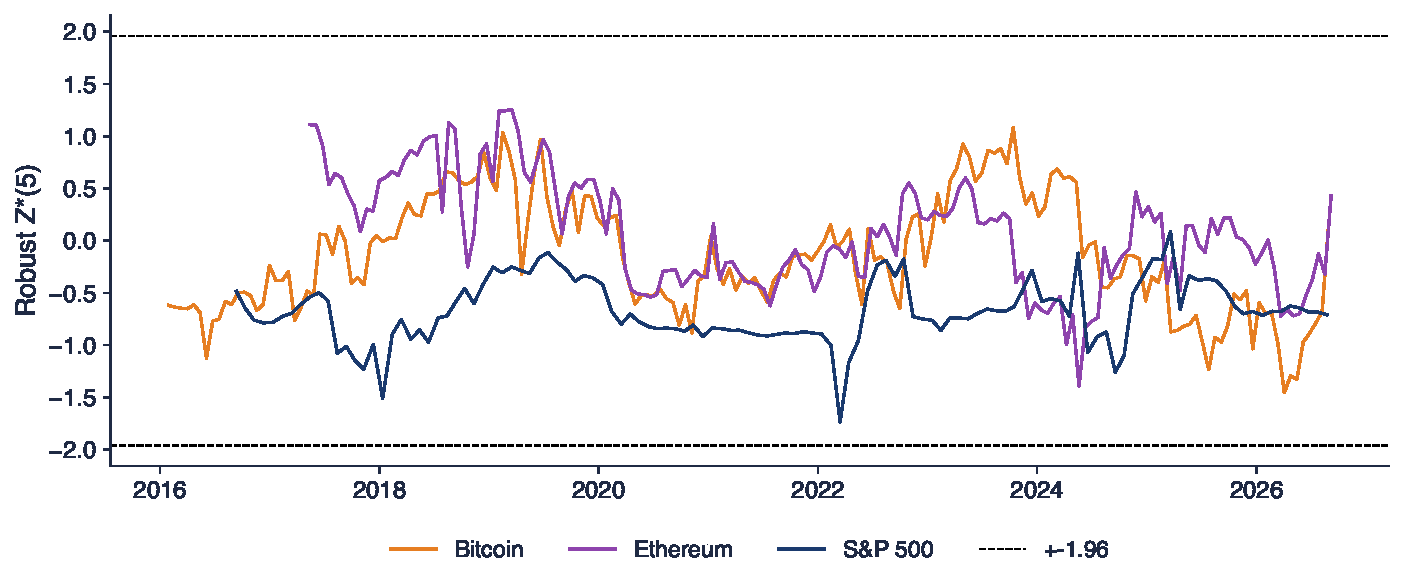
\includegraphics[width=0.97\textwidth,height=0.46\textheight,keepaspectratio]{sfm_ch14_rolling_vr.pdf}
\end{center}
\vspace{-0.25cm}
\begin{itemize}
    \item Robust $Z^*(5)$ on windows of 500 observations, one window every 21 observations (as in \sfmchlink{https://danpele.github.io/SFM/EN/Courses/chapter7_efficient_markets_random_walk_vr.pdf}{Chapter 7})
    \item Interpretation: Bitcoin 0.0\% of 185 windows reject; with the i.i.d.\ statistic $Z(5)$ the share would be 1.6\% for Bitcoin and 21.7\% for the S\&P 500: ignoring volatility clustering creates false rejections
\end{itemize}
\sfmquantlet{Ch_14}{SFM_ch14_garch_efficiency}
\end{frame}

\begin{frame}{How Efficiency Evolved}
\itemsize{\small}
\begin{itemize}
    \item \refUrquhart: Bitcoin was inefficient in 2010--2016 as a whole, but moved towards efficiency after 2013
    \begin{itemize}
        \item \refNC: a power transformation of the same returns passes the tests: the early verdict was fragile
        \item \refTL: an adjusted measure of inefficiency; crypto markets became more efficient after 2017
    \end{itemize}
    \item Our data (since 2014): VR(5) between 0.78 and 1.17 on rolling windows; no robust rejection
    \begin{itemize}
        \item the market grew, arbitrageurs arrived, derivatives and ETFs appeared: the adaptive-markets view of \sfmchlink{https://danpele.github.io/SFM/EN/Courses/chapter11_fractal_markets_long_memory.pdf}{Chapter 11}
    \end{itemize}
    \item Weak-form efficiency is not efficiency in general: prices can be unpredictable and still be far from any fundamental value
\end{itemize}
\end{frame}

\begin{frame}{Case Study: Trading and Arbitrage Across Exchanges}
\itemsize{\small}
\begin{itemize}
    \item \refMS: tick data of 34 exchanges in 19 countries, 2017--2018
    \begin{itemize}
        \item \textbf{arbitrage}: buy where the price is low, sell where it is high; in an efficient market the gap closes fast
    \end{itemize}
    \item Findings
    \begin{itemize}
        \item large and persistent price gaps between countries (Korea, Japan and the United States), much smaller within a country
        \item the gaps open when Bitcoin rises and capital controls make the arbitrage hard
        \item a common component explains most of the order flow: prices are driven by one global market
    \end{itemize}
    \item Lesson: the ``law of one price'' fails where money cannot move freely; a statistical test on one series cannot see this
\end{itemize}
\end{frame}

\begin{frame}{Case Study: Is Bitcoin Really Untethered?}
\itemsize{\small}
\begin{itemize}
    \item \refGS: blockchain records of Bitcoin and of the stablecoin Tether (USDT), 2017--2018
    \begin{itemize}
        \item question: was new USDT used to buy Bitcoin after price falls?
    \end{itemize}
    \item Findings
    \begin{itemize}
        \item purchases with Tether came after market falls and were followed by price rises
        \item the flows came mostly from one large account on one exchange (Bitfinex)
        \item hours with such flows account for a large share of the 2017 rise
    \end{itemize}
    \item Related: manipulation of the Mt.~Gox exchange in 2013 \refGHMO. Lesson: blockchain data allow tests that are impossible in equity markets
\end{itemize}
\end{frame}

\begin{frame}{Recap: Is the Crypto Market Efficient?}
\itemsize{\small}
\begin{itemize}
    \item Robust VR tests do not reject the random walk for Bitcoin and Ethereum since 2014
    \item Early studies found inefficiency; the market became more efficient as it grew
    \item Arbitrage gaps across countries and manipulation show the limits of weak-form tests
\end{itemize}
\end{frame}


%=============================================================================
\section{Correlation with Equities and Gold}
%=============================================================================

\begin{frame}{Measuring Correlation Across Calendars}
\itemsize{\small}
\begin{itemize}
    \item Bitcoin trades 7 days a week, the S\&P 500 and gold 5: first join the \textbf{prices} on common days, then compute returns
    \begin{itemize}
        \item Monday's Bitcoin return then covers Friday to Monday, like the S\&P 500 return
        \item joining returns instead would drop the weekend moves of Bitcoin
    \end{itemize}
    \item \textbf{Asynchronous} closes: Bitcoin at midnight UTC, the S\&P 500 at 16:00 New York time
    \begin{itemize}
        \item weekly returns (Friday to Friday) reduce this problem; we report both
    \end{itemize}
    \item \textbf{Rolling correlation}: the sample correlation on the last 250 common days, recomputed every day
    \begin{itemize}
        \item standard error about $(1 - \rho^2)/\sqrt{250} \approx 0.06$: moves below 0.1 are noise
    \end{itemize}
\end{itemize}
\end{frame}

\begin{frame}{Rolling Correlation with Equities and Gold}
\itemsize{\footnotesize}
\begin{center}
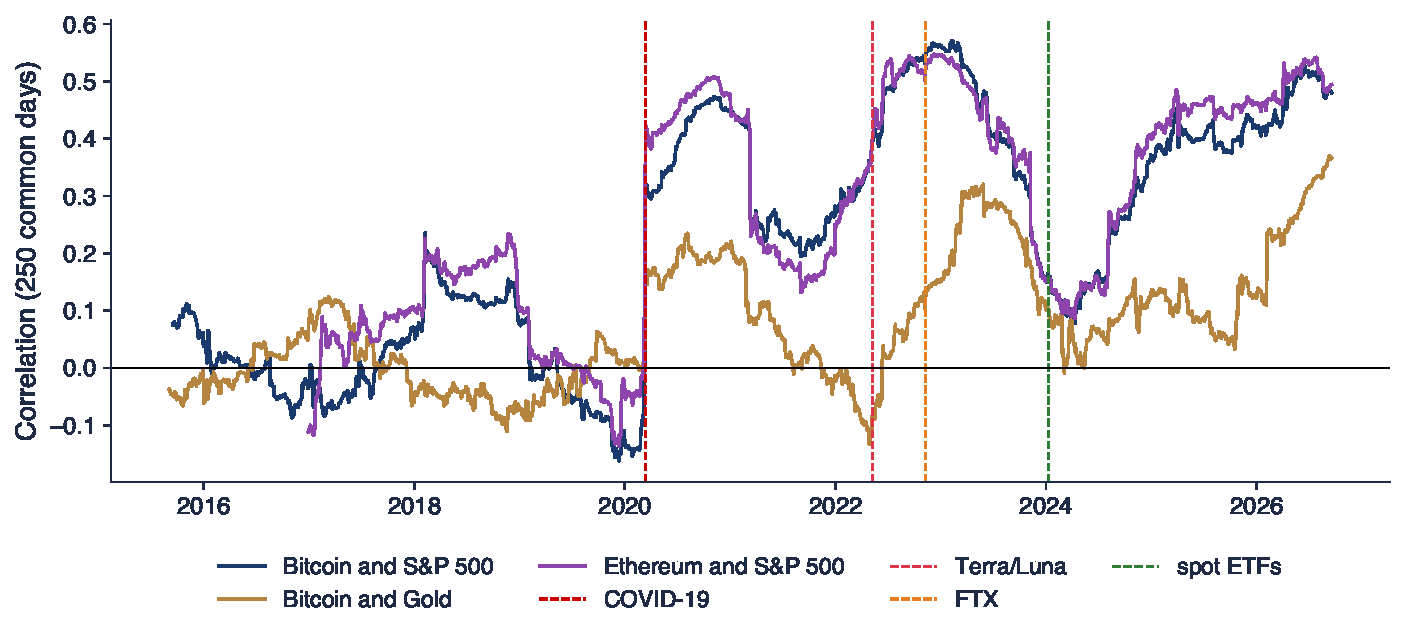
\includegraphics[width=0.97\textwidth,height=0.48\textheight,keepaspectratio]{sfm_ch14_rolling_corr.pdf}
\end{center}
\vspace{-0.25cm}
\begin{itemize}
    \item Daily log returns on common days; 250-day windows; dashed: COVID-19, Terra/Luna, FTX and the spot ETFs
    \item Interpretation: Bitcoin and the S\&P 500 were uncorrelated before 2020 (0.02) and positively correlated after (0.39); the maximum, 0.57, came on 9 February 2023; gold stays weakly linked
\end{itemize}
\sfmquantlet{Ch_14}{SFM_ch14_correlation}
\end{frame}

\begin{frame}{Correlation Year by Year}
\itemsize{\footnotesize}
\begin{center}
\scriptsize
\begin{tabular}{lrrrrrrr}
\toprule
Bitcoin with & 2019 & 2020 & 2021 & 2022 & 2023 & 2024 & 2025 \\
\midrule
S\&P 500 & $-0.11$ & $0.45$ & $0.26$ & $0.56$ & $0.16$ & $0.36$ & $0.42$ \\
gold & $0.01$ & $0.21$ & $-0.02$ & $0.15$ & $0.12$ & $0.12$ & $0.12$ \\
Ethereum with S\&P 500 & $-0.02$ & $0.47$ & $0.20$ & $0.55$ & $0.15$ & $0.40$ & $0.46$ \\
\bottomrule
\end{tabular}
\end{center}
\begin{itemize}
    \item Whole period: daily 0.24, weekly 0.19 for Bitcoin and the S\&P 500
    \begin{itemize}
        \item the asynchronous closes do not explain the correlation: weekly returns give a similar number
    \end{itemize}
    \item Interpretation
    \begin{itemize}
        \item since 2020, crypto behaves as a risk asset: it falls with equities when interest rates rise (2022)
        \item the change coincides with the arrival of institutional investors; a diversification benefit measured before 2020 no longer holds
    \end{itemize}
\end{itemize}
\end{frame}

\begin{frame}{Three Crisis Episodes}
\itemsize{\footnotesize}
\begin{center}
\scriptsize
\begin{tabular}{llrrrrr}
\toprule
Episode & period & Bitcoin & Ethereum & S\&P 500 & gold & worst Bitcoin day \\
\midrule
COVID-19 & 19 February 2020 -- 23 March 2020 & $-40.6$ & $-65.5$ & $-41.4$ & $0.3$ & $-46.5$ \\
Terra/Luna & 5 May 2022 -- 12 May 2022 & $-23.0$ & $-33.8$ & $-5.4$ & $-3.0$ & $-11.7$ \\
FTX & 5 November 2022 -- 21 November 2022 & $-29.9$ & $-38.4$ & $4.6$ & $3.4$ & $-15.5$ \\
\bottomrule
\end{tabular}
\end{center}
\begin{itemize}
    \item Cumulative log returns in \% from the first to the last close; worst day: the smallest daily log return of Bitcoin
    \item Interpretation
    \begin{itemize}
        \item COVID-19 (a global shock): crypto fell as much as equities, gold did not move
        \item Terra/Luna (May 2022) and FTX (an exchange that went bankrupt in November 2022): crypto-specific shocks; crypto fell by a quarter or more, the S\&P 500 much less or not at all
        \item the dependence is asymmetric: equity crashes reach crypto, crypto crashes rarely reach equities
    \end{itemize}
\end{itemize}
\end{frame}

\begin{frame}{Hedge or Safe Haven?}
\itemsize{\small}
\begin{itemize}
    \item \refBL: a \textbf{hedge} is uncorrelated or negatively correlated with equities on average; a \textbf{safe haven} is so in market crashes
    \begin{itemize}
        \item test: the mean return on the worst 5\% of S\&P 500 days (151 common days, S\&P 500 below $-1.65\%$, on average $-2.70\%$)
    \end{itemize}
    \item Bitcoin: $-2.77\%$ on those days ($t = -4.89$, p $<$\,0.001); negative on 70\% of them
    \begin{itemize}
        \item gold: 0.10\% ($t = 0.86$, p 0.394)
    \end{itemize}
    \item Interpretation: Bitcoin is not a safe haven; on the worst equity days it falls as much as the S\&P 500; gold holds its value
    \item The ``digital gold'' narrative is not supported by the data of this sample
\end{itemize}
\end{frame}

\begin{frame}{Recap: Correlation with Equities and Gold}
\itemsize{\small}
\begin{itemize}
    \item Join prices on common days, then compute returns; check weekly returns
    \item Correlation with equities: about 0 before 2020, about 0.39 after
    \item Bitcoin is neither a hedge nor a safe haven for equities in this sample
\end{itemize}
\end{frame}


%=============================================================================
\section{Bubbles and Crashes}
%=============================================================================

\begin{frame}{Drawdown}
\itemsize{\small}
\begin{itemize}
    \item \textbf{Drawdown}: $D_t = P_t/\max_{s \le t} P_s - 1$, the loss from the last record high (\sfmchlink{https://danpele.github.io/SFM/EN/Courses/chapter1_data_returns_indicators.pdf}{Chapter 1})
    \begin{itemize}
        \item \textbf{maximum drawdown}: $\min_t D_t$; \textbf{time under water}: the days until a new record high
    \end{itemize}
    \item A loss of $d$ needs a gain of $d/(1 - d)$ to recover
    \begin{itemize}
        \item $d = 75\%$: $0.75/0.25 = 300\%$; $d = 80\%$: 400\%
        \item Bitcoin's deepest drawdown in our data: $-83.4\%$ (15 December 2018); recovery needed a gain of 502\%
    \end{itemize}
    \item Drawdowns depend on the path, not only on the distribution of returns: high volatility and clustering produce deep ones
\end{itemize}
\end{frame}

\begin{frame}{Drawdowns of Bitcoin, Ethereum and the S\&P 500}
\itemsize{\footnotesize}
\begin{center}
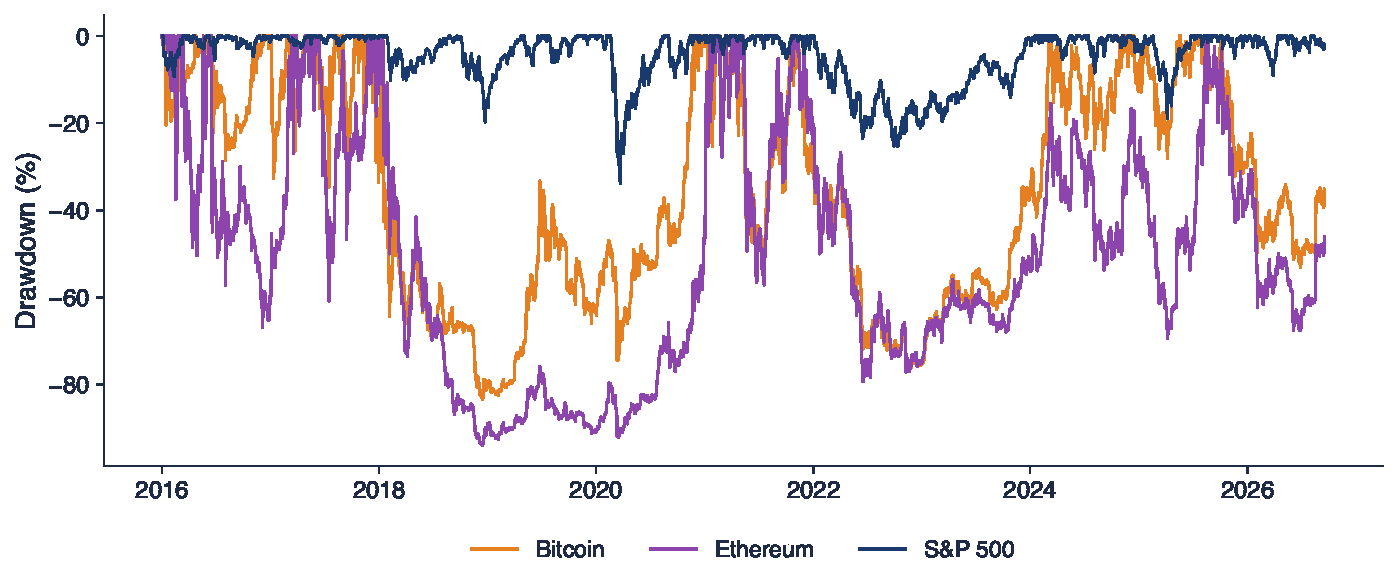
\includegraphics[width=0.97\textwidth,height=0.46\textheight,keepaspectratio]{sfm_ch14_drawdowns.pdf}
\end{center}
\vspace{-0.25cm}
\begin{itemize}
    \item Daily closes since 2016; maximum drawdowns: Bitcoin $-83.4\%$, Ethereum $-94.0\%$, S\&P 500 $-33.9\%$
    \item Interpretation: Bitcoin spent 76\% of the days more than 10\% below its record, Ethereum 90\%, the S\&P 500 16\%; on 18 September 2026 Bitcoin was 35.2\% below its record
\end{itemize}
\sfmquantlet{Ch_14}{SFM_ch14_bubbles_etf}
\end{frame}

\begin{frame}{Bitcoin's Large Drawdowns}
\itemsize{\footnotesize}
\begin{center}
\scriptsize
\begin{tabular}{lrlrrlr}
\toprule
Peak & USD & trough & USD & depth (\%) & new record & days under water \\
\midrule
2014-09-17 & 457 & 2015-01-14 & 178 & $-61.1$ & 2015-12-15 & 454 \\
2017-12-16 & 19\,497 & 2018-12-15 & 3\,237 & $-83.4$ & 2020-11-30 & 1080 \\
2021-04-13 & 63\,503 & 2021-07-20 & 29\,807 & $-53.1$ & 2021-10-19 & 189 \\
2021-11-08 & 67\,567 & 2022-11-21 & 15\,787 & $-76.6$ & 2024-03-04 & 847 \\
2025-10-06 & 124\,753 & 2026-06-30 & 58\,559 & $-53.1$ & not yet & -- \\
\bottomrule
\end{tabular}
\end{center}
\begin{itemize}
    \item Episodes since September 2014 whose drawdown exceeded 50\%; dates as year-month-day
    \item Interpretation
    \begin{itemize}
        \item 5 falls of more than half in twelve years: a crash of this size is a regular event, not a rare one
        \item the 2017 and 2021 peaks were recovered after 1080 and 847 days
    \end{itemize}
\end{itemize}
\end{frame}

\begin{frame}{Bubbles and the Log-Periodic Idea}
\itemsize{\footnotesize}
\begin{columns}[T]
\begin{column}{0.66\textwidth}
\begin{itemize}
    \item \textbf{Bubble}: a price far above the fundamental value, sustained by the expectation of selling higher
    \begin{itemize}
        \item \refCF: the fundamental value of Bitcoin is zero; its price shows speculative bubbles
    \end{itemize}
    \item Log-periodic power law (LPPL) \refJLS: before a crash, $\ln P_t \approx A + B(t_c - t)^m + C(t_c - t)^m\cos(\omega\ln(t_c - t) - \phi)$
    \begin{itemize}
        \item faster than exponential growth with accelerating oscillations; $t_c$: the critical time
    \end{itemize}
    \item Caution: seven parameters, many local optima, and $t_c$ is the most uncertain of them; fits look convincing only after the crash
\end{itemize}
\end{column}
\begin{column}{0.31\textwidth}
\centering
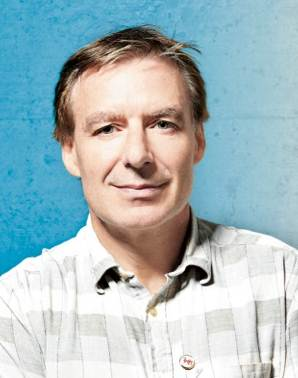
\includegraphics[height=0.36\textheight]{ch14_sornette_2012.jpg}\\[1mm]
\imgcap{Didier Sornette}
\imgcredit{https://commons.wikimedia.org/wiki/File:Didier_Sornette.jpg}{Photo: Didier Sornette (2012); CC BY-SA 3.0 DE; Wikimedia Commons}
\end{column}
\end{columns}
\end{frame}

\begin{frame}{Recap: Bubbles and Crashes}
\itemsize{\small}
\begin{itemize}
    \item Drawdown $= P_t/\max P - 1$; a fall of $d$ needs a gain of $d/(1 - d)$
    \item Bitcoin lost more than half of its value 5 times since 2014
    \item Bubble models are useful descriptions, unreliable for timing a crash
\end{itemize}
\end{frame}


%=============================================================================
\section{Spot Bitcoin ETFs}
%=============================================================================

\begin{frame}{January 2024: Bitcoin Enters the Stock Exchange}
\itemsize{\footnotesize}
\begin{columns}[T]
\begin{column}{0.62\textwidth}
\begin{itemize}
    \item \textbf{ETF} (exchange-traded fund): a fund whose shares trade on a stock exchange; \textbf{spot}: it holds the asset itself, not futures
    \begin{itemize}
        \item 10 January 2024: the SEC (Securities and Exchange Commission) approves 11 spot Bitcoin ETFs \refSEC; trading starts on 11 January
    \end{itemize}
    \item Why it matters
    \begin{itemize}
        \item pension funds and advisers can hold Bitcoin through a regulated security
        \item ETF shares trade only on weekdays: part of the trading moves to stock-market hours
    \end{itemize}
    \item Statistical question: did Bitcoin's volatility, its weekend pattern or its link with equities change?
\end{itemize}
\end{column}
\begin{column}{0.35\textwidth}
\centering
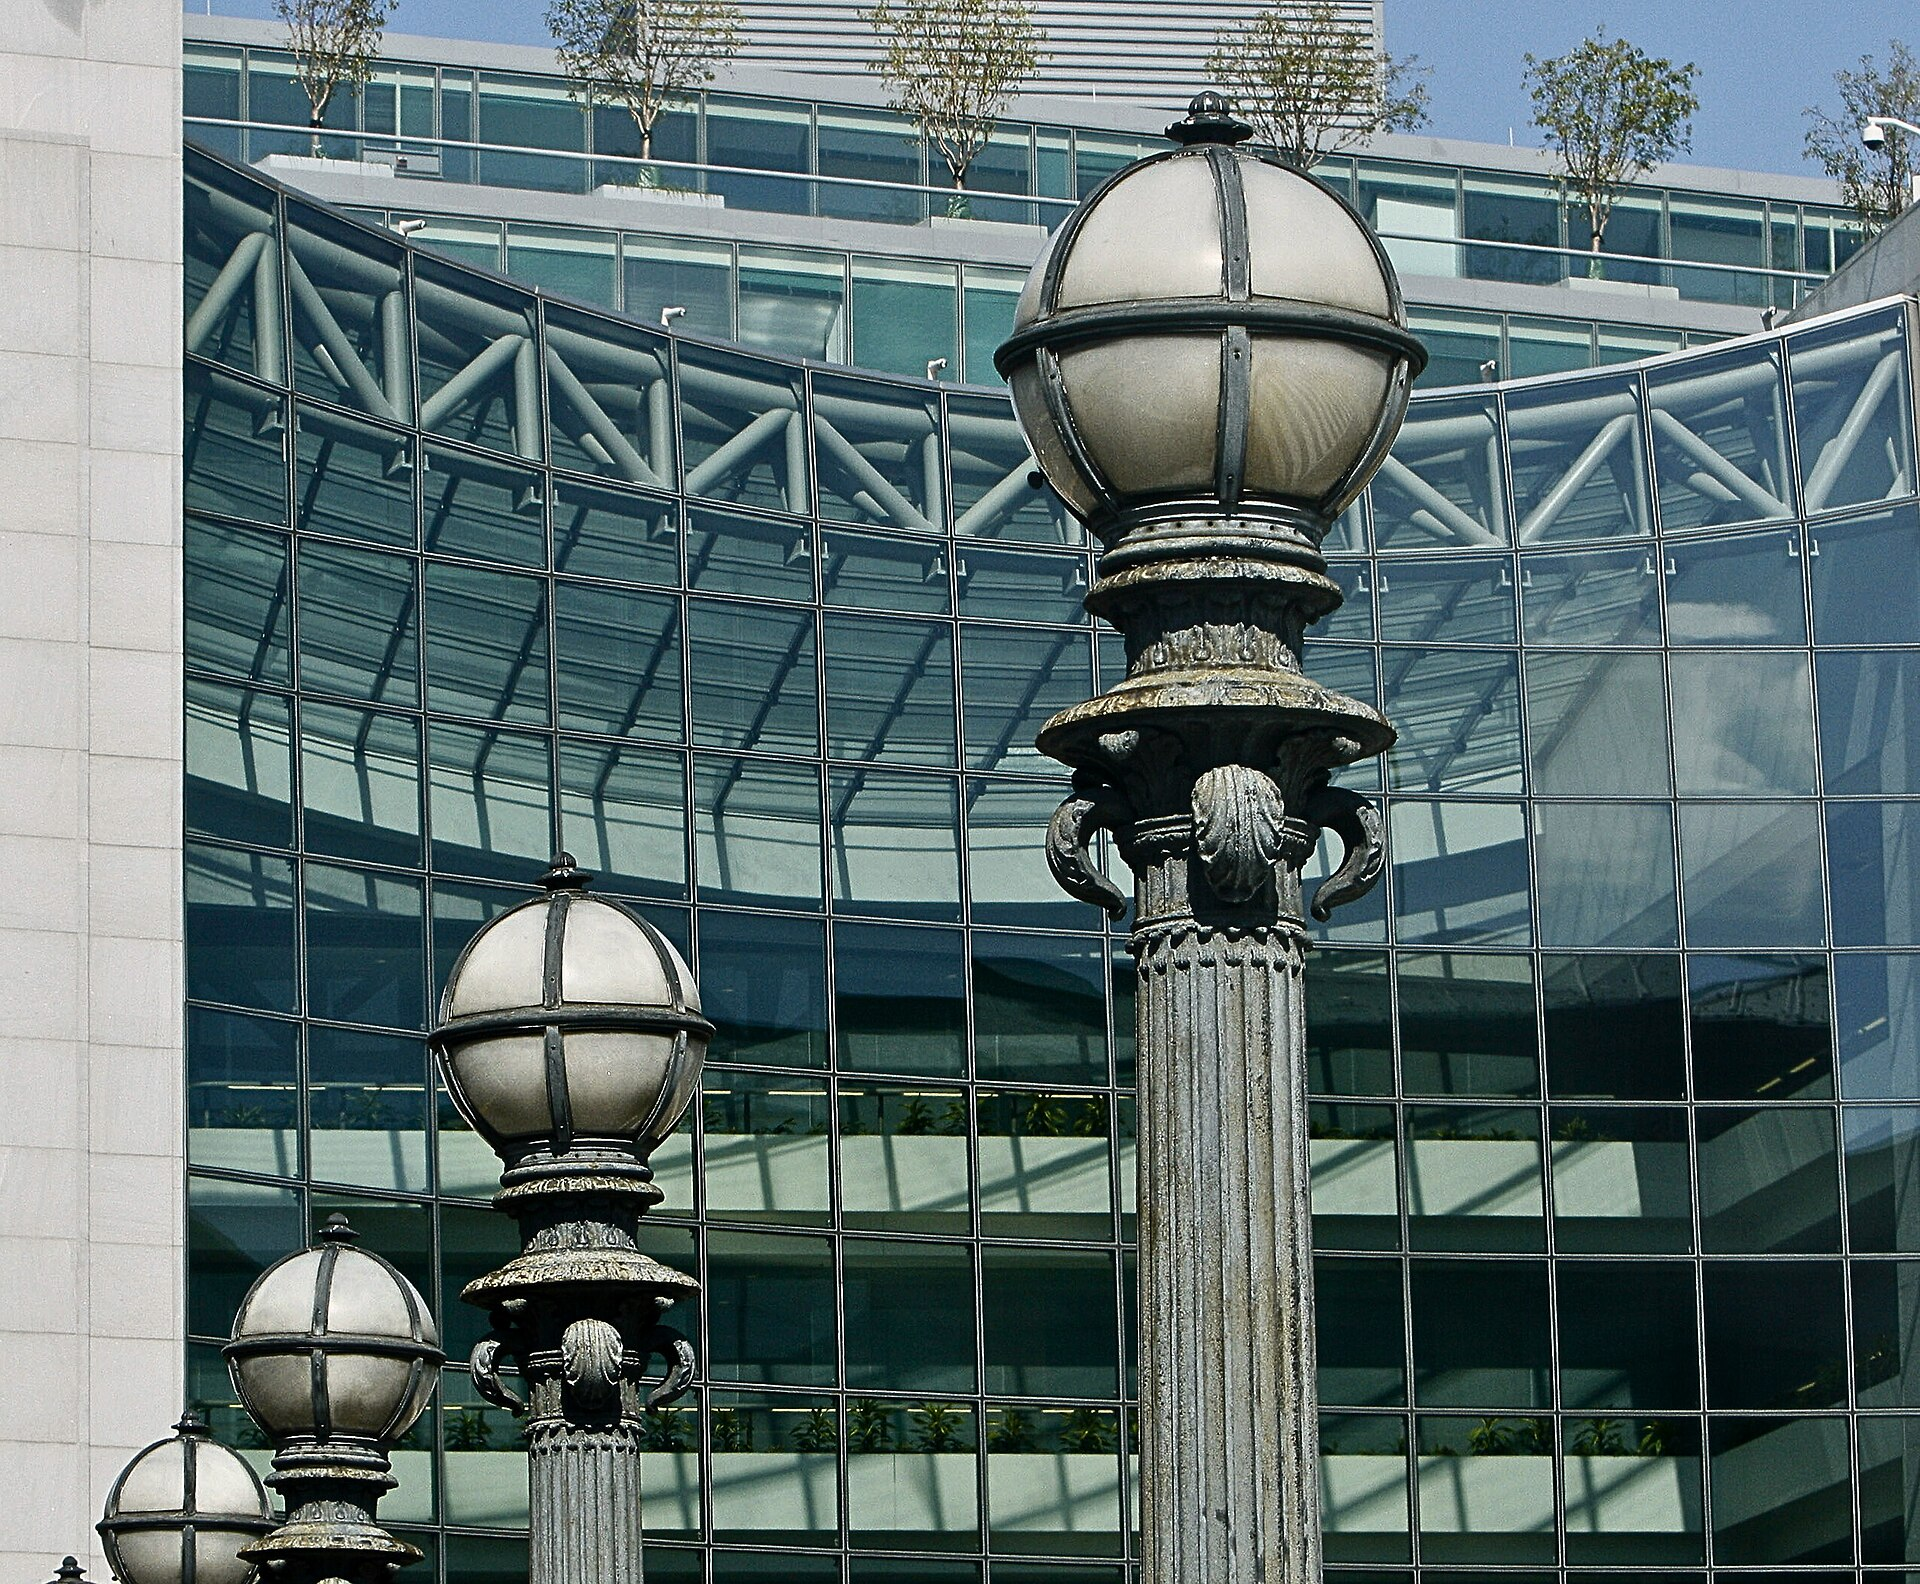
\includegraphics[height=0.34\textheight]{ch14_sec_hq_2008.jpg}\\[1mm]
\imgcap{SEC headquarters, Washington, D.C.}
\imgcredit{https://commons.wikimedia.org/wiki/File:Facade_of_the_U.S._Securities_and_Exchange_Commission_headquarters,_Washington,_D.C.jpg}{Photo: David (dbking) (2008); CC BY 2.0; Wikimedia Commons}
\end{column}
\end{columns}
\end{frame}

\begin{frame}{Volatility and the Weekend Share Around the ETFs}
\itemsize{\footnotesize}
\begin{center}
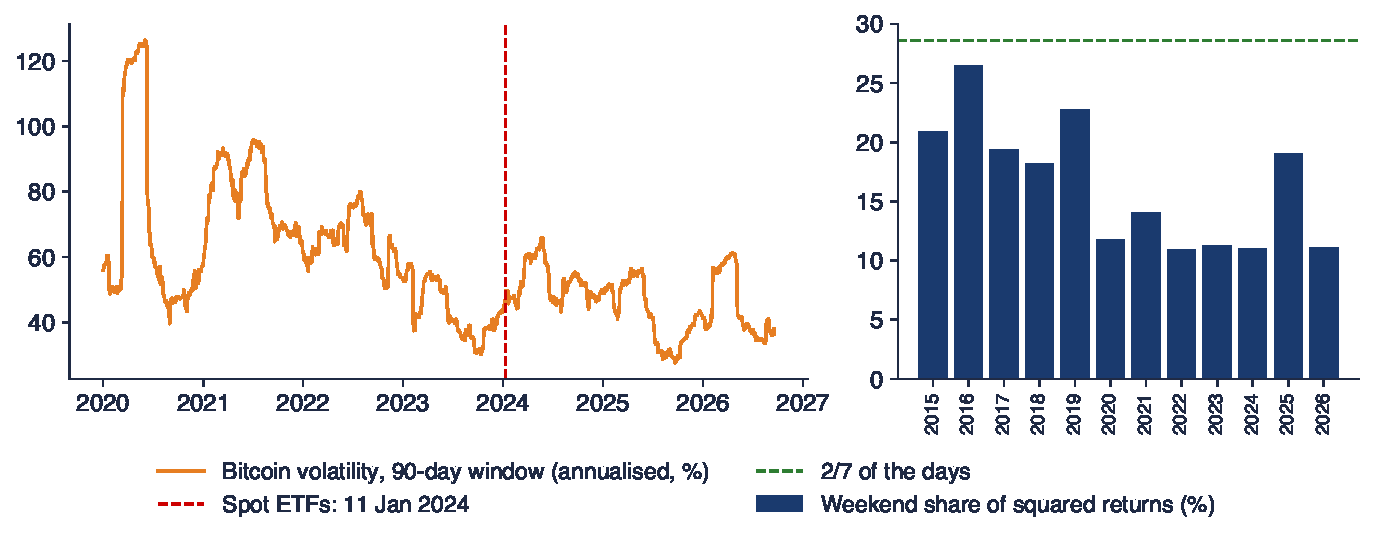
\includegraphics[width=0.97\textwidth,height=0.46\textheight,keepaspectratio]{sfm_ch14_etf.pdf}
\end{center}
\vspace{-0.25cm}
\begin{itemize}
    \item Left: Bitcoin volatility on 90-day windows, annualised with $\sqrt{365}$. Right: weekend share of the sum of squared returns by year (2/7 if every day had the same variance)
    \item Interpretation: volatility kept falling after January 2024, but it was already falling before; the weekend share has been well below 2/7 since 2020
\end{itemize}
\sfmquantlet{Ch_14}{SFM_ch14_bubbles_etf}
\end{frame}

\begin{frame}{Before and After: a Simple Comparison}
\itemsize{\footnotesize}
\begin{center}
\footnotesize
\begin{tabular}{lrr}
\toprule
Bitcoin & two years before & two years after \\
\midrule
annualised volatility (\%) & $55.2$ & $47.5$ \\
weekend/weekday variance & $0.30$ & $0.42$ \\
correlation with the S\&P 500 & $0.45$ & $0.37$ \\
GARCH(1,1)-t $\hat\alpha + \hat\beta$ & $1.000$ & $0.97$ \\
\bottomrule
\end{tabular}
\end{center}
\begin{itemize}
    \item Windows: 11 January 2022 -- 10 January 2024 (729 days) and 11 January 2024 -- 10 January 2026 (730 days)
    \item Brown--Forsythe test of equal variance: statistic 1.22, p $= 0.27$: the fall in volatility is not significant
    \item Interpretation
    \begin{itemize}
        \item a before--after comparison is not a causal effect: interest rates, the halving of April 2024 and the US election changed at the same time
        \item a credible study needs a control group (e.g.\ coins without an ETF) or intraday data around the opening of the stock exchange
    \end{itemize}
\end{itemize}
\end{frame}

\begin{frame}{How Well Does an ETF Track Bitcoin?}
\itemsize{\small}
\begin{itemize}
    \item IBIT (iShares Bitcoin Trust), adjusted close, and Bitcoin, prices joined on the 671 trading days of the ETF
    \begin{itemize}
        \item correlation of daily returns 0.91; slope of IBIT on Bitcoin 0.94
        \item \textbf{tracking error}: the annualised standard deviation of the return difference, 20.8\%
    \end{itemize}
    \item Why not 1: the two closes are four hours apart (16:00 in New York against midnight UTC)
    \begin{itemize}
        \item over a week the difference averages out; the fund itself holds Bitcoin one to one, minus a small fee
    \end{itemize}
    \item Lesson: a high tracking error can be a measurement artefact; align the times before judging a fund
\end{itemize}
\end{frame}

\begin{frame}{Recap: Spot Bitcoin ETFs}
\itemsize{\small}
\begin{itemize}
    \item January 2024: Bitcoin becomes available through regulated ETFs
    \item Volatility fell (55.2\% to 47.5\%), not significantly; causality is not identified
    \item Asynchronous closing times inflate the tracking error of daily returns
\end{itemize}
\end{frame}


%=============================================================================
\section{Stablecoins}
%=============================================================================

\begin{frame}{What Is a Stablecoin?}
\itemsize{\footnotesize}
\begin{center}
\scriptsize
\begin{tabular}{>{\raggedright\arraybackslash}p{2.2cm}>{\raggedright\arraybackslash}p{4.4cm}>{\raggedright\arraybackslash}p{2.0cm}>{\raggedright\arraybackslash}p{2.4cm}}
\toprule
Type & how the peg is held & examples & risk \\
\midrule
fiat-backed & reserves of dollars, deposits and Treasury bills; holders redeem 1 coin for 1 USD at the issuer & USDT, USDC & the reserves and the bank that holds them \\
crypto-backed & over-collateralised loans in crypto, liquidated automatically by smart contracts & DAI & a crash of the collateral \\
algorithmic & no reserves: an algorithm mints and burns a second coin to keep the price at 1 USD & UST (Terra) & a run that destroys both coins \\
\bottomrule
\end{tabular}
\end{center}
\begin{itemize}
    \item \textbf{Stablecoin}: a crypto asset designed to keep a fixed price, usually 1 USD (the \textbf{peg})
    \begin{itemize}
        \item used as cash on crypto exchanges and for payments across borders; DefiLlama classifies today 91.3\% of the supply as fiat-backed, 8.7\% as crypto-backed
    \end{itemize}
\end{itemize}
\end{frame}

\begin{frame}{How a Peg Is Held: Arbitrage}
\itemsize{\small}
\begin{itemize}
    \item Primary market: authorised traders create a coin for 1 USD at the issuer, or redeem it for 1 USD
    \begin{itemize}
        \item price 0.99 on exchanges: buy at 0.99, redeem at 1.00, profit 1 cent: demand pushes the price back up
        \item price 1.01: create at 1.00, sell at 1.01: supply pushes the price down
    \end{itemize}
    \item \refLVN: the peg of Tether holds because of this arbitrage; premiums appear when traders flee into stablecoins in crypto downturns
    \begin{itemize}
        \item \refMZZ: with few authorised arbitrageurs, runs are less likely but deviations last longer
    \end{itemize}
    \item The arbitrage works only while traders trust that redemption at 1 USD will be honoured: a peg is a promise
\end{itemize}
\end{frame}

\begin{frame}{Supply of Stablecoins}
\itemsize{\footnotesize}
\begin{center}
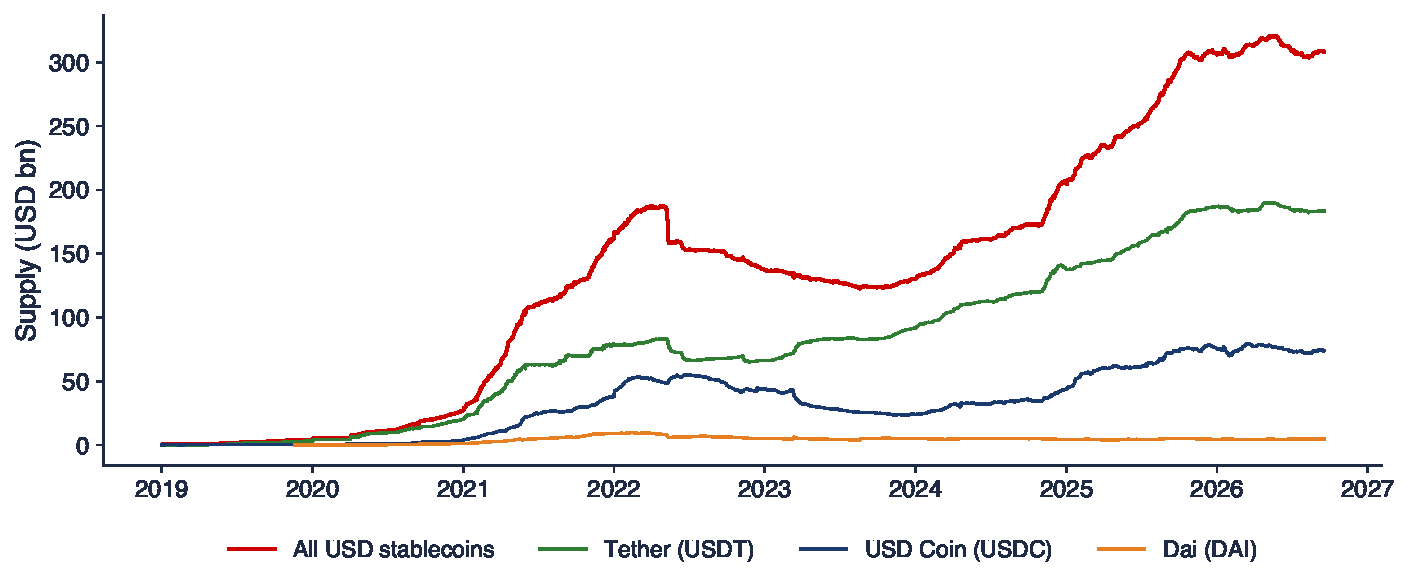
\includegraphics[width=0.97\textwidth,height=0.44\textheight,keepaspectratio]{sfm_ch14_stablecoin_supply.pdf}
\end{center}
\vspace{-0.25cm}
\begin{itemize}
    \item Circulating supply in billion USD (DefiLlama): all USD stablecoins, USDT, USDC and DAI
    \item Interpretation: from 4.2 billion USD at the start of 2020 to 308 billion on 18 September 2026, a factor of 74; USDT holds 60\%, USDC 24\%
    \item The total fell from 187 billion (2 April 2022) to 123 billion (19 August 2023) after Terra and FTX; USDC fell from 43 to 24 billion in 2023
\end{itemize}
\sfmquantlet{Ch_14}{SFM_ch14_stablecoins}
\end{frame}

\begin{frame}{Peg Deviation in Basis Points}
\itemsize{\small}
\begin{itemize}
    \item \textbf{Basis point} (bp): one hundredth of a percent, 0.01\% $= 0.0001$
    \begin{itemize}
        \item \textbf{peg deviation}: $d_t = 10\,000\,(P_t - 1)$ bp for a coin pegged to 1 USD
    \end{itemize}
    \item \textbf{Worked example}: USDC closed at 0.9715 USD on 11 March 2023
    \begin{itemize}
        \item $d = 10\,000 \times (0.9715 - 1) = -285$ bp, a loss of 2.85\%
        \item a holder of 1\,000\,000 USDC who sold at that close lost 28\,500 USD; at the daily low (0.8774): 122\,600 USD
    \end{itemize}
    \item Statistics of a peg: the median absolute deviation, the share of days beyond 10 or 50 bp, the worst close and the worst low
    \begin{itemize}
        \item speed of return: AR(1) $d_t = \phi\,d_{t-1} + e_t$, half-life $\ln 0.5/\ln\phi$ days
    \end{itemize}
\end{itemize}
\end{frame}

\begin{frame}{Peg Deviations of USDT, USDC and DAI}
\itemsize{\footnotesize}
\begin{center}
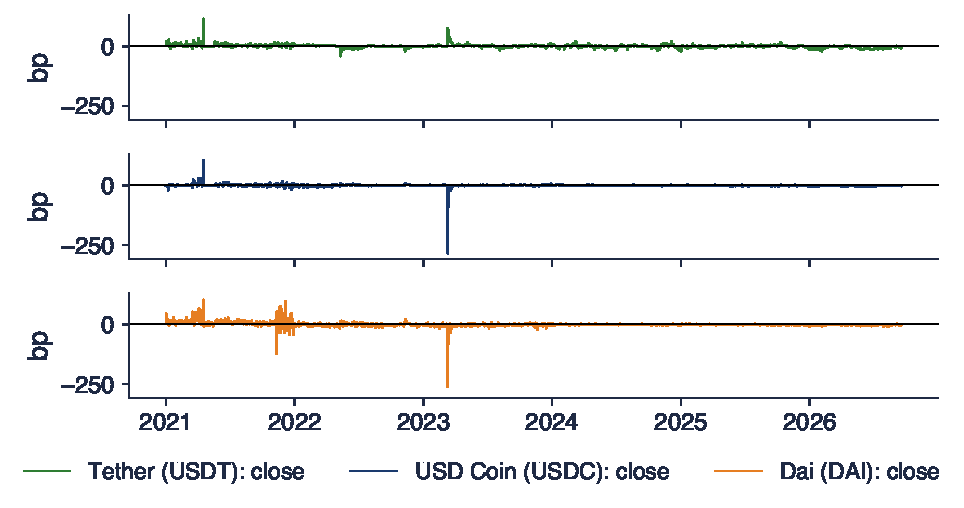
\includegraphics[width=0.97\textwidth,height=0.48\textheight,keepaspectratio]{sfm_ch14_peg.pdf}
\end{center}
\vspace{-0.25cm}
\begin{itemize}
    \item Daily closing deviation from 1 USD in bp since 2021 (EODHD)
    \item Median absolute deviation: USDT 3.1 bp, USDC 1.1 bp, DAI 2.2 bp; days beyond 10 bp: 11.4\%, 1.5\%, 10.7\%
    \item Interpretation: half-lives of 2.2, 0.6 and 0.6 days: deviations close within days; the exception is March 2023 (USDC $-285$ bp, DAI $-261$ bp)
\end{itemize}
\sfmquantlet{Ch_14}{SFM_ch14_stablecoins}
\end{frame}

\begin{frame}{March 2023: USDC and Silicon Valley Bank}
\itemsize{\footnotesize}
\begin{columns}[T]
\begin{column}{0.62\textwidth}
\begin{itemize}
    \item 10 March 2023: Silicon Valley Bank (SVB) is closed by its regulator \refFDIC; part of the cash reserves of USDC was deposited there
    \begin{itemize}
        \item a weekend follows: banks are closed, crypto markets are open
    \end{itemize}
    \item 11 March: USDC falls to 0.8774 USD (low, $-1226$ bp) and closes at 0.9715; DAI, backed largely by USDC, follows
    \begin{itemize}
        \item USDT trades above 1 (close up to 77 bp): money flees from one stablecoin into another
    \end{itemize}
    \item 12 March, evening: US authorities guarantee all SVB deposits \refFed; on 13 March USDC is back at the peg
\end{itemize}
\end{column}
\begin{column}{0.35\textwidth}
\centering
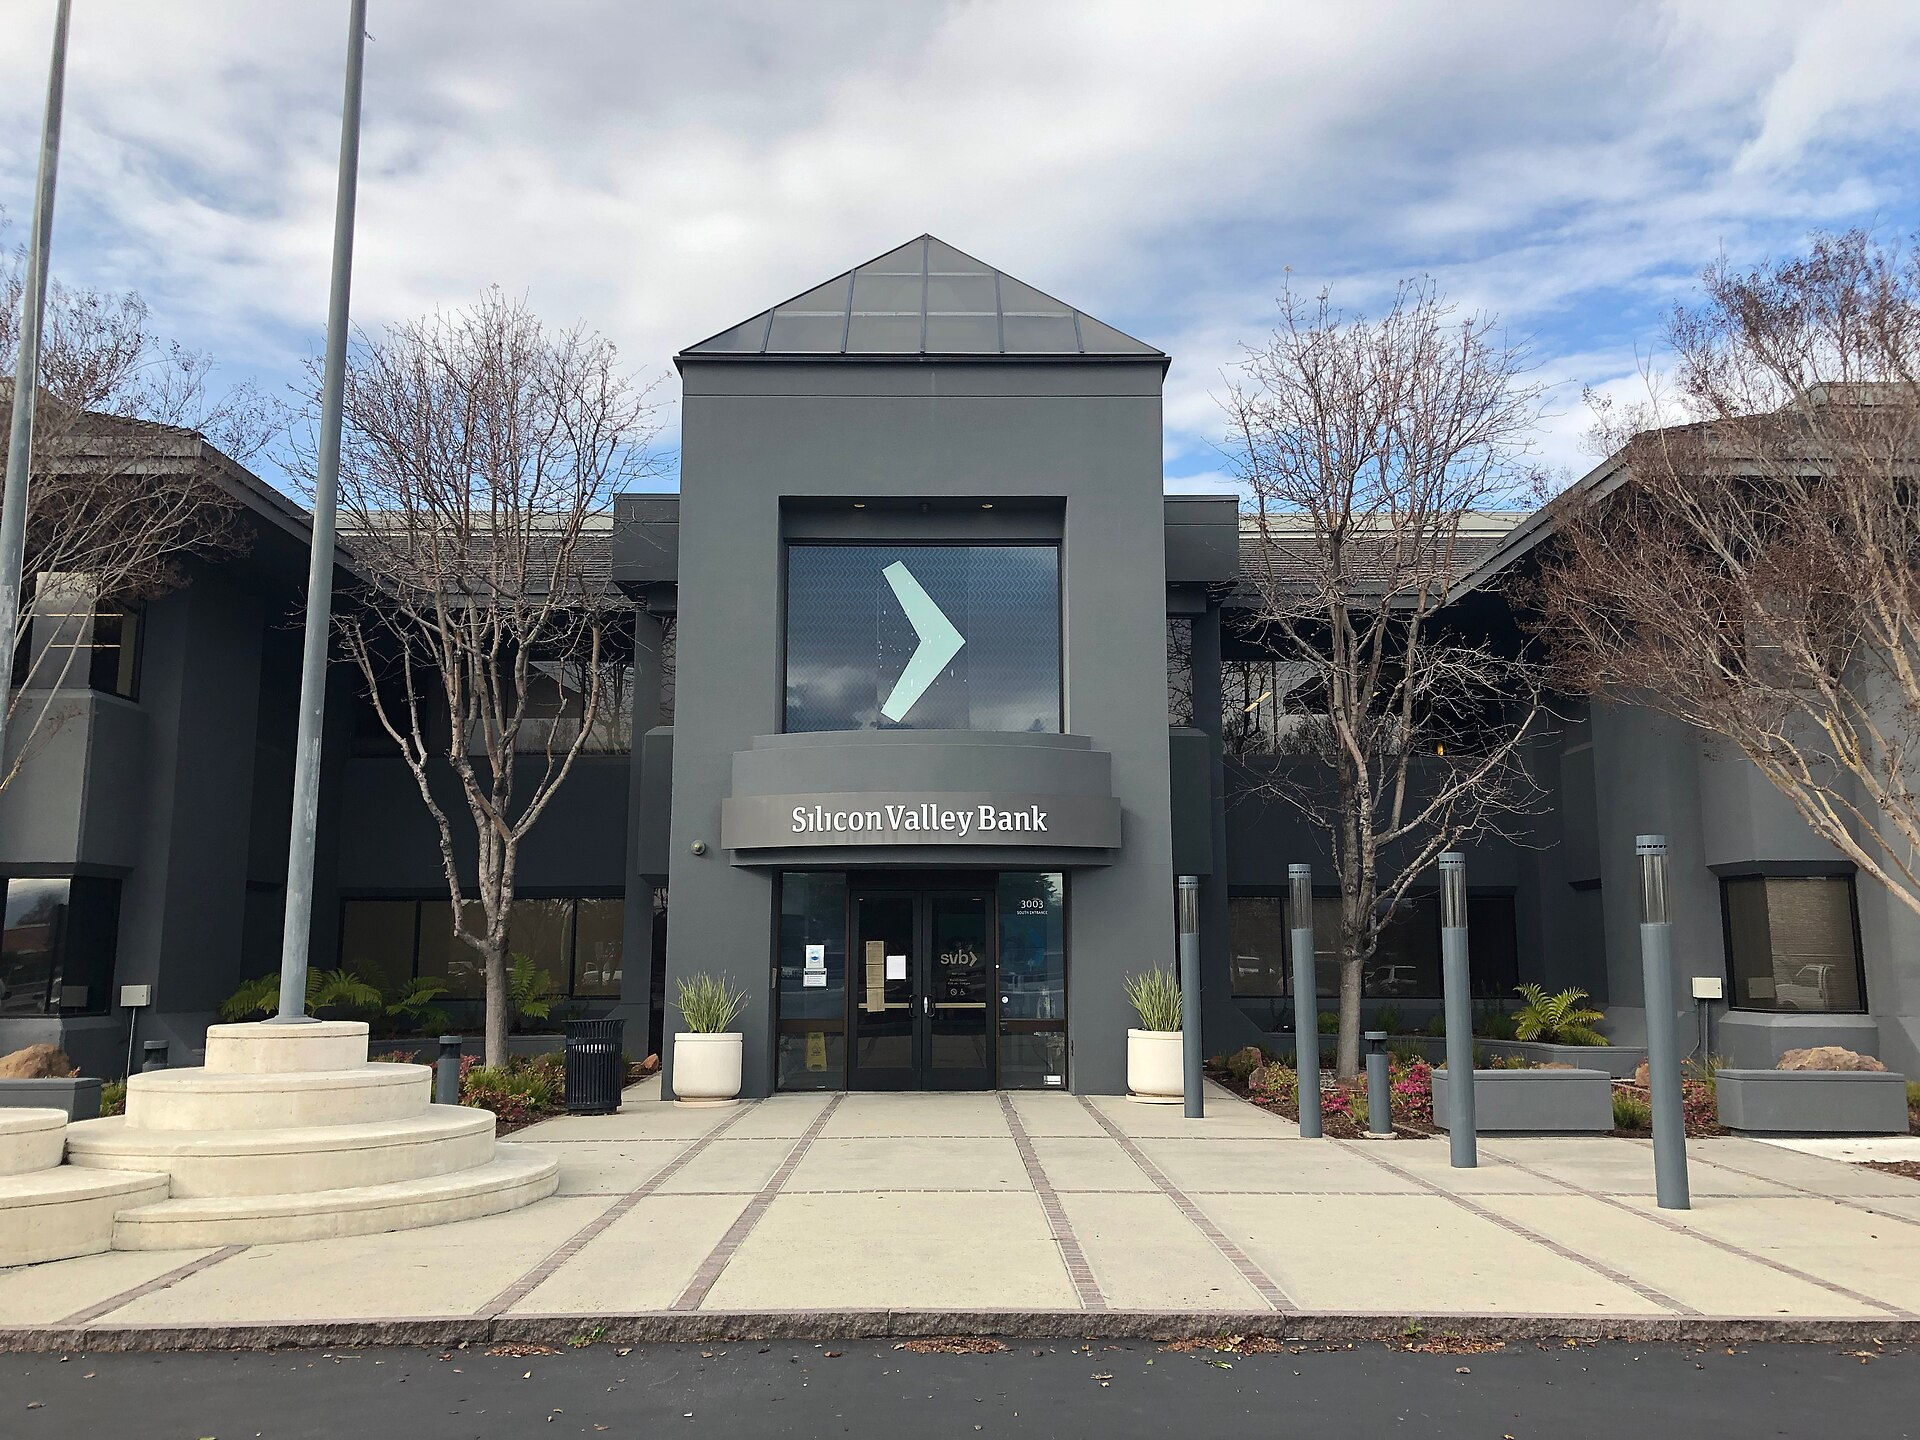
\includegraphics[height=0.34\textheight]{ch14_svb_hq_2023.jpg}\\[1mm]
\imgcap{SVB headquarters, Santa Clara, 13 March 2023}
\imgcredit{https://commons.wikimedia.org/wiki/File:3003_West_Tasman_Drive_entrance_2,_Santa_Clara,_California.jpg}{Photo: Minh Nguyen (2023); CC BY-SA 4.0; Wikimedia Commons}
\end{column}
\end{columns}
\end{frame}

\begin{frame}{The USDC Depeg, Day by Day}
\itemsize{\footnotesize}
\begin{center}
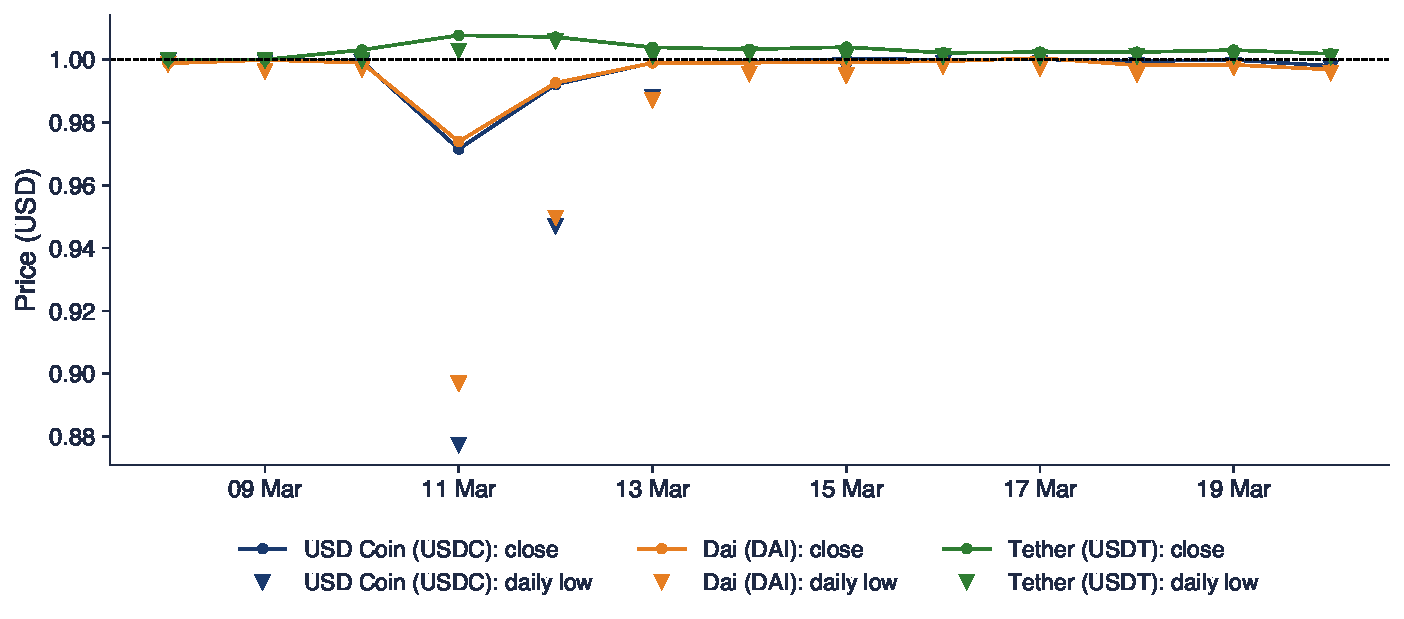
\includegraphics[width=0.97\textwidth,height=0.48\textheight,keepaspectratio]{sfm_ch14_svb.pdf}
\end{center}
\vspace{-0.25cm}
\begin{itemize}
    \item Daily closes (circles) and lows (triangles), 8--20 March 2023; dashed: the peg
    \item Interpretation: a fiat-backed coin is as safe as its bank: the peg broke when the reserves were in doubt and returned when the deposits were guaranteed; the run was on the reserves, not on the code
\end{itemize}
\sfmquantlet{Ch_14}{SFM_ch14_stablecoins}
\end{frame}

\begin{frame}{TerraUSD: an Algorithmic Stablecoin}
\itemsize{\small}
\begin{itemize}
    \item UST was kept at 1 USD by a swap with a second coin, LUNA: 1 UST could always be exchanged for 1 USD worth of LUNA
    \begin{itemize}
        \item UST below 1: buy UST, swap it for 1 USD of new LUNA, sell the LUNA: UST is burned, LUNA is minted
        \item the only backing was the market value of LUNA
    \end{itemize}
    \item Demand came from the Anchor protocol, which paid close to 20\% a year on UST deposits \refLMS
    \begin{itemize}
        \item UST supply peaked at 18.8 billion on 7 May 2022
    \end{itemize}
    \item The \textbf{death spiral}: large withdrawals from Anchor, UST below 1, more LUNA minted, LUNA falls, the backing shrinks, more withdrawals
    \begin{itemize}
        \item \refLMS: large, sophisticated holders withdrew first; small holders were the last to leave
    \end{itemize}
\end{itemize}
\end{frame}

\begin{frame}{The Collapse of UST, May 2022}
\itemsize{\footnotesize}
\begin{center}
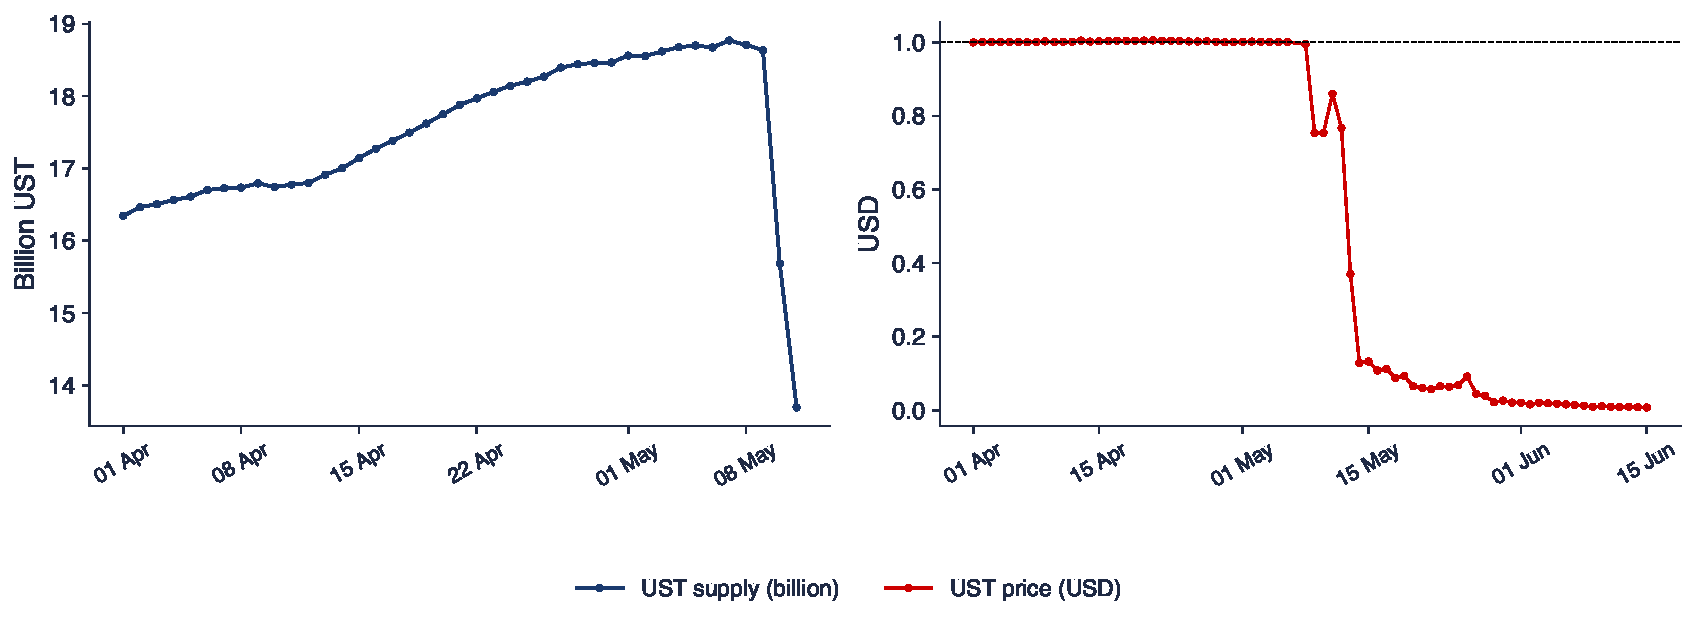
\includegraphics[width=0.97\textwidth,height=0.44\textheight,keepaspectratio]{sfm_ch14_ust.pdf}
\end{center}
\vspace{-0.25cm}
\begin{itemize}
    \item DefiLlama: UST supply until the last published day (11 May 2022) and the daily UST price
    \item Interpretation: the price was 0.75 USD on 9 May, 0.37 on 13 May, 0.13 on 14 May and 0.02 on 31 May; the supply fell by 27\% in four days, from 7 to 11 May
    \item Unlike USDC, there was no reserve and no lender of last resort: an algorithmic peg cannot be rescued
\end{itemize}
\sfmquantlet{Ch_14}{SFM_ch14_stablecoins}
\end{frame}

\begin{frame}{Stablecoins as Private Money}
\itemsize{\small}
\begin{itemize}
    \item \refGZ: stablecoins resemble the banknotes of private US banks in the ``wildcat banking'' era (1837--1863)
    \begin{itemize}
        \item notes of different banks traded at different discounts, depending on trust in each bank
        \item remedy then: a uniform national currency; remedy proposed now: regulate stablecoins as bank deposits
    \end{itemize}
    \item \refGorton: the peg holds as long as holders value the coin for trading with leverage in crypto markets
    \begin{itemize}
        \item when that demand disappears, the coin trades below par, like a bank note of an uncertain bank
    \end{itemize}
    \item Statistical lesson: peg deviations are small and short in normal times and jump in a crisis: a heavy-tailed, regime-dependent series
\end{itemize}
\end{frame}

\begin{frame}{Regulation in the European Union: MiCA}
\itemsize{\footnotesize}
\begin{columns}[T]
\begin{column}{0.62\textwidth}
\begin{itemize}
    \item MiCA, Markets in Crypto-Assets \refMiCA, adopted in 2023
    \begin{itemize}
        \item rules for stablecoins apply from 30 June 2024; for other crypto-asset services from 30 December 2024 \refESMA
    \end{itemize}
    \item Stablecoins pegged to one currency are \textbf{e-money tokens}
    \begin{itemize}
        \item issued only by authorised credit or e-money institutions; redemption at par at any time; no interest to holders
        \item reserves kept separate and invested in safe, liquid assets
    \end{itemize}
    \item Algorithmic stablecoins without reserves have no place in this framework
\end{itemize}
\end{column}
\begin{column}{0.35\textwidth}
\centering
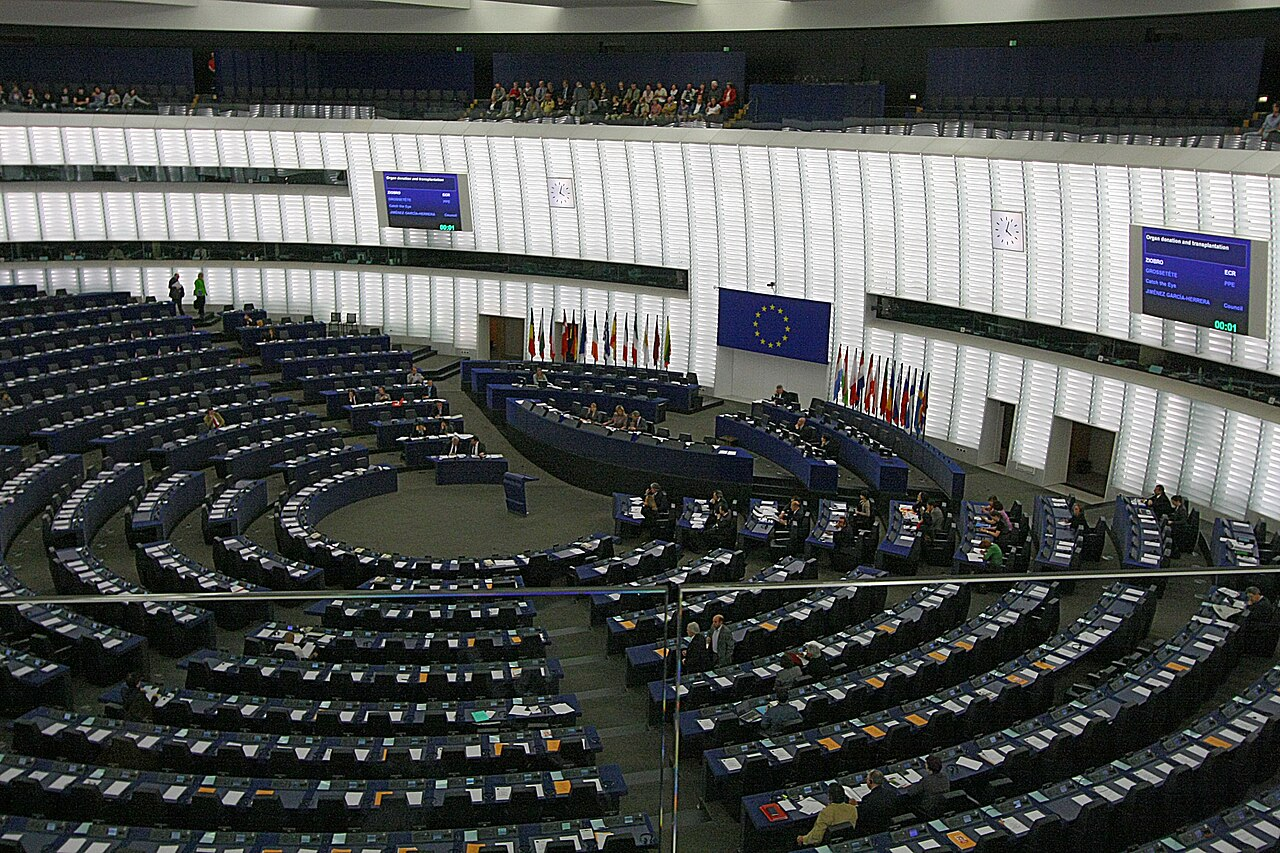
\includegraphics[height=0.30\textheight]{ch14_eu_parliament_2010.jpg}\\[1mm]
\imgcap{European Parliament, Strasbourg}
\imgcredit{https://commons.wikimedia.org/wiki/File:Hemicycle_of_Louise_Weiss_building_of_the_European_Parliament,_Strasbourg.jpg}{Photo: jeffowenphotos (2010); CC BY 2.0; Wikimedia Commons}
\end{column}
\end{columns}
\end{frame}

\begin{frame}{Regulation in the United States: the GENIUS Act}
\itemsize{\footnotesize}
\begin{columns}[T]
\begin{column}{0.62\textwidth}
\begin{itemize}
    \item GENIUS Act (Guiding and Establishing National Innovation for U.S. Stablecoins Act), signed on 18 July 2025 \refGENIUS
    \begin{itemize}
        \item payment stablecoins: reserves of at least 1 USD per coin, in cash, deposits and short-term Treasury bills
        \item monthly public reports on the reserves; no interest paid to holders
    \end{itemize}
    \item Common points of MiCA and GENIUS: full reserves, redemption at par, supervision of issuers
    \begin{itemize}
        \item they address the run on reserves of March 2023 and the algorithmic collapse of May 2022
    \end{itemize}
    \item A fully reserved stablecoin is close to a narrow bank: safe, but its issuer earns the interest on the reserves
\end{itemize}
\end{column}
\begin{column}{0.35\textwidth}
\centering
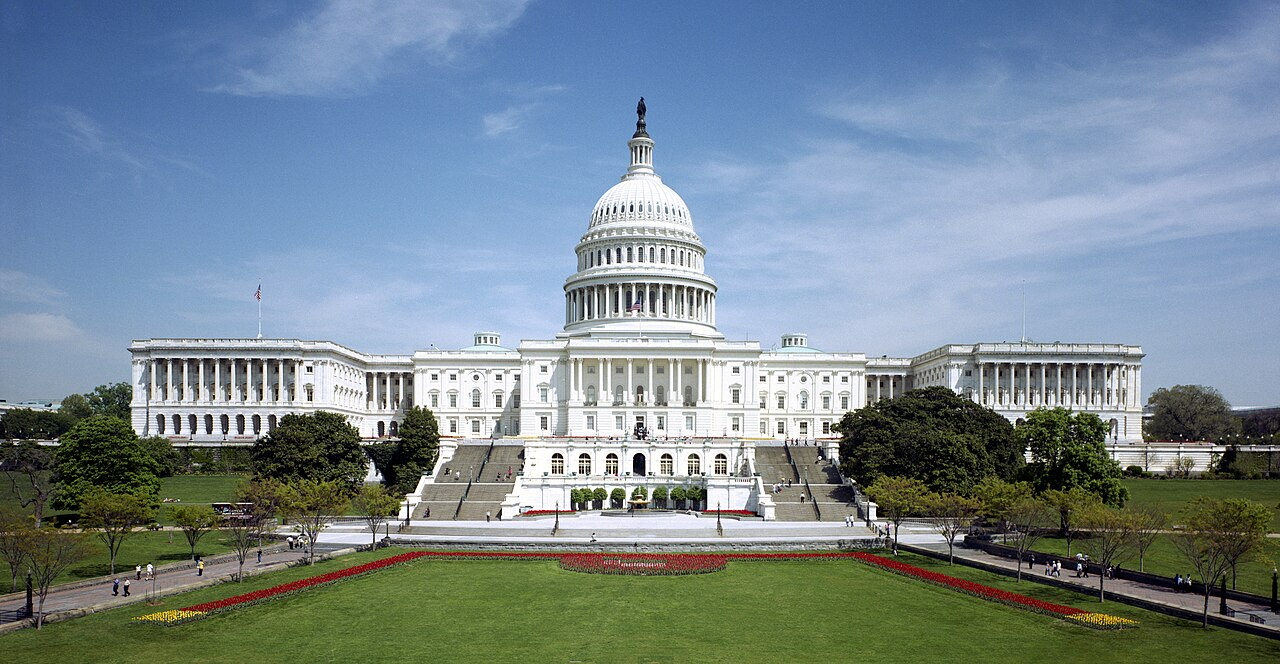
\includegraphics[height=0.24\textheight]{ch14_us_capitol.jpg}\\[1mm]
\imgcap{United States Capitol, Washington, D.C.}
\imgcredit{https://commons.wikimedia.org/wiki/File:United_States_Capitol_-_west_front.jpg}{Photo: Architect of the Capitol; public domain; Wikimedia Commons}
\end{column}
\end{columns}
\end{frame}

\begin{frame}{Recap: Stablecoins}
\itemsize{\small}
\begin{itemize}
    \item Three types: fiat-backed, crypto-backed, algorithmic; a supply of 308 billion USD in September 2026
    \item Peg deviation in bp: $10\,000(P - 1)$; small and short-lived, except in crises
    \item USDC (2023): a run on the reserves, rescued; UST (2022): no reserves, collapse; MiCA and GENIUS require full reserves
\end{itemize}
\end{frame}


%=============================================================================
\section{The Risk of a Crypto Position}
%=============================================================================

\begin{frame}{VaR 1\% and ES 2.5\% in Dollars}
\itemsize{\small}
\begin{itemize}
    \item \sfmchlink{https://danpele.github.io/SFM/EN/Courses/chapter10_var_es_backtesting.pdf}{Chapter 10}: $\mathrm{VaR}_\alpha = -q_\alpha$, the loss exceeded with probability $\alpha$ (VaR 1\%); $\mathrm{ES}_\alpha = -E[r \mid r \le q_\alpha]$ (ES 2.5\%)
    \begin{itemize}
        \item historical simulation (HS), Normal, Student-t (maximum likelihood), GARCH(1,1)-t for the next day
    \end{itemize}
    \item From log returns to dollars: a log return of $-v\%$ means a loss of $W(1 - e^{-v/100})$ on a position of value $W$
    \begin{itemize}
        \item Bitcoin, HS: VaR 1\% $= 10.54\%$; $W = 100\,000$ USD: $100\,000 \times (1 - 0.8999) = 10\,006$ USD
    \end{itemize}
    \item Horizon: crypto trades every day, so a 10-day VaR covers 10 calendar days, not two trading weeks
\end{itemize}
\end{frame}

\begin{frame}{Four Methods, Three Assets}
\itemsize{\scriptsize}
\begin{center}
\scriptsize
\begin{tabular}{lrrrrrrrr}
\toprule
& \multicolumn{4}{c}{VaR 1\% (\%)} & \multicolumn{4}{c}{ES 2.5\% (\%)} \\ & HS & Normal & t & GARCH-t & HS & Normal & t & GARCH-t \\
\midrule
Bitcoin & $10.54$ & $7.99$ & $11.06$ & $7.37$ & $10.84$ & $8.03$ & $13.37$ & $8.11$ \\
Ethereum & $14.29$ & $11.40$ & $15.39$ & $10.95$ & $14.77$ & $11.45$ & $18.13$ & $12.05$ \\
S\&P 500 & $3.26$ & $2.54$ & $3.04$ & $1.78$ & $3.50$ & $2.55$ & $3.45$ & $1.86$ \\
\bottomrule
\end{tabular}
\end{center}
\begin{center}
\scriptsize
\begin{tabular}{lrrrr}
\toprule
Position of 100\,000 USD & VaR 1\% HS & ES 2.5\% HS & VaR 1\% Normal & 10-day VaR 1\% HS \\
\midrule
Bitcoin & 10\,006 & 10\,277 & 7\,679 & 25\,563 \\
Ethereum & 13\,312 & 13\,732 & 10\,772 & 31\,842 \\
S\&P 500 & 3\,204 & 3\,438 & 2\,506 & 9\,049 \\
\bottomrule
\end{tabular}
\end{center}
\begin{itemize}
    \item Whole samples until 18 September 2026; t: Student-t by maximum likelihood ($\hat\nu = 2.23$ for Bitcoin); GARCH-t: the forecast for the next day ($\hat\sigma = 2.83\%$)
\end{itemize}
\end{frame}

\begin{frame}{Interpretation of the Risk Numbers}
\itemsize{\small}
\begin{itemize}
    \item A Bitcoin position is about three times as risky as an S\&P 500 position: VaR 1\% 10.54\% against 3.26\%
    \begin{itemize}
        \item the Normal VaR 1\% is 24\% below the historical one for Bitcoin: heavy tails again
    \end{itemize}
    \item Conditional against unconditional: GARCH-t gives 7.37\% today, below the historical 10.54\%, because volatility is now low
    \begin{itemize}
        \item the historical number is a long-run average; the GARCH number is today's risk
    \end{itemize}
    \item 10 days: the historical VaR 1\% of 10-day returns is 29.52\%; the square-root-of-time rule gives 33.34\%
    \begin{itemize}
        \item the rule overstates: with tail index $\alpha > 2$, an extreme quantile of a sum of $h$ returns grows roughly like $h^{1/\alpha}$, more slowly than $\sqrt{h}$
    \end{itemize}
    \item ES 2.5\% (HS) is close to VaR 1\% (HS) for Bitcoin, as in \sfmchlink{https://danpele.github.io/SFM/EN/Courses/chapter10_var_es_backtesting.pdf}{Chapter 10} for equities
\end{itemize}
\end{frame}

\begin{frame}{Backtesting Bitcoin VaR 1\%}
\itemsize{\footnotesize}
\begin{center}
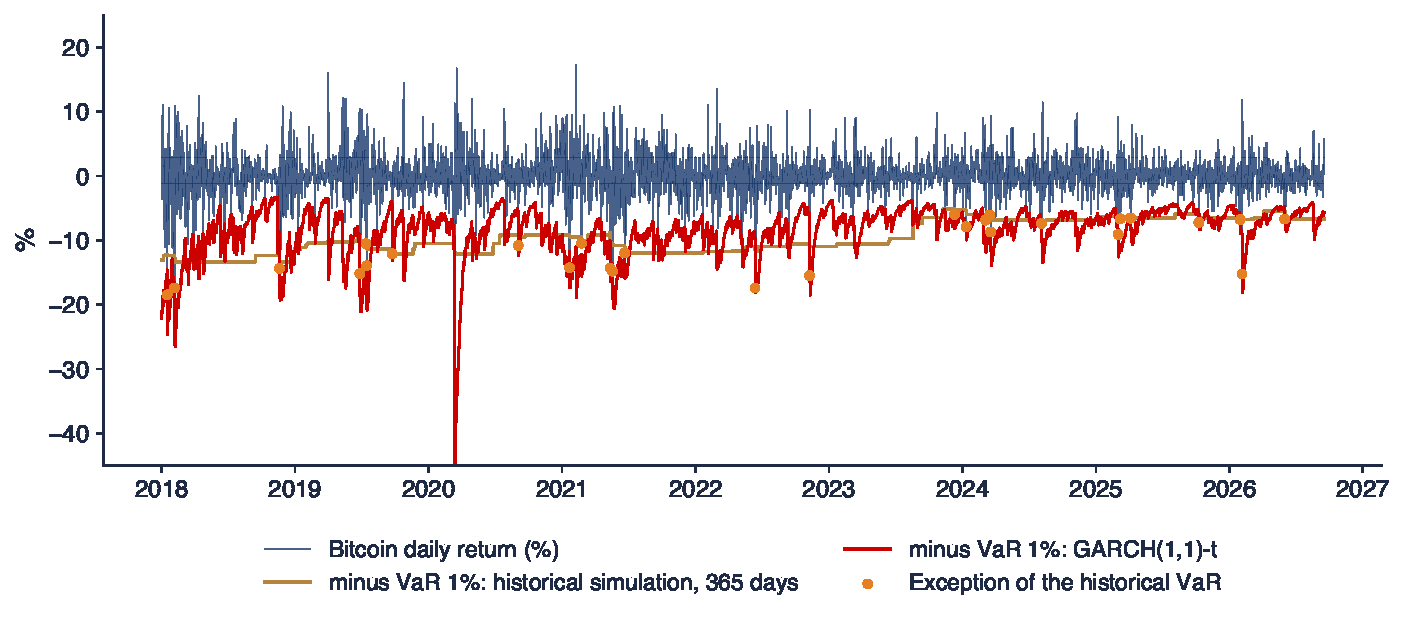
\includegraphics[width=0.97\textwidth,height=0.44\textheight,keepaspectratio]{sfm_ch14_btc_var.pdf}
\end{center}
\vspace{-0.25cm}
\begin{itemize}
    \item One-day forecasts since 1 January 2018: HS on the last 365 days; GARCH(1,1)-t re-estimated every 365 days on all earlier data
    \item Exceptions (expected 31.8): HS 29 (0.91\%), GARCH-t 41 (1.29\%); Kupiec \refKupiec: $LR = 0.26$ (p $= 0.61$) and $2.45$ (p $= 0.12$)
    \item Interpretation: both pass the Kupiec test; HS needs a higher VaR on average (9.5\% against 8.5\%), GARCH-t reacts faster but is exceeded more often (2018: 9 exceptions)
\end{itemize}
\sfmquantlet{Ch_14}{SFM_ch14_crypto_var}
\end{frame}

\begin{frame}{Recap: The Risk of a Crypto Position}
\itemsize{\small}
\begin{itemize}
    \item Convert log-return VaR to money with $W(1 - e^{-v/100})$
    \item Bitcoin VaR 1\% is about three times that of the S\&P 500; the Normal understates it
    \item Historical simulation and GARCH-t both pass the backtest since 2018
\end{itemize}
\end{frame}


%=============================================================================
\section{AI for Scientific Discovery}
%=============================================================================

\begin{frame}{An Open Question}
\itemsize{\small}
\begin{itemize}
    \item \textbf{Do stablecoin flows move crypto prices?}
    \begin{itemize}
        \item \refGS{} found that Tether issuance supported Bitcoin in 2017; the stablecoin market is now about 74 times larger than in 2020
        \item starter result: weekly log change of the stablecoin supply against Bitcoin's return, 349 weeks since 2020
    \end{itemize}
    \item Same week: correlation 0.26; next week: 0.07, slope 0.19 ($t = 1.20$, p $= 0.23$, $R^2 = 0.4\%$)
    \begin{itemize}
        \item flows and prices move together; flows do not predict the next week: cause, effect or common demand?
    \end{itemize}
    \item AI tools can speed up such a study; they do not replace checking it \refWang
\end{itemize}
\end{frame}

\begin{frame}{How AI Could Help}
\itemsize{\small}
\begin{itemize}
    \item \textbf{Literature}: a list of studies on stablecoin issuance and crypto prices, with their data and periods
    \item \textbf{Data}: code that downloads the supply of each stablecoin from DefiLlama and aligns it with daily prices
    \item \textbf{Robustness}: daily and weekly data, USDT and USDC separately, sub-periods, Granger causality in both directions
    \item Example prompt
    \begin{itemize}
        \item \aiprompt{Write Python code that downloads the daily supply of USDT and USDC from the DefiLlama stablecoins API, computes weekly log changes, joins them with weekly Bitcoin log returns, and tests whether supply changes Granger-cause returns and returns Granger-cause supply changes, with HAC standard errors.}
    \end{itemize}
\end{itemize}
\end{frame}

\begin{frame}{What to Check}
\itemsize{\small}
\begin{itemize}
    \item Annualisation: 365 days for crypto, 252 for equities; never one number for both
    \item Alignment: prices joined on common days before returns; the same week definition for both series
    \item Units: basis points against percent (285 bp $= 2.85\%$); billions against millions in supply data
    \item VaR convention: VaR 1\% is a positive loss; never ``VaR 99\%''
    \item Look-ahead: the supply series must be known at the date of the forecast; revisions of the data provider count
    \item References: every cited paper must exist; check the DOI
\end{itemize}
\end{frame}

\begin{frame}{Project Idea}
\itemsize{\small}
\begin{itemize}
    \item \textbf{Question}: do weekly changes in USDT and USDC supply help to forecast Bitcoin's return or volatility, and did this change after the spot ETFs?
    \begin{itemize}
        \item data: DefiLlama supply (public, no key) and the course data for prices
    \end{itemize}
    \item Steps
    \begin{itemize}
        \item weekly log changes; correlation and Granger tests in both directions with HAC standard errors
        \item out-of-sample forecasts of next week's return and of the absolute return, against a random walk
        \item sub-periods: before and after Terra (May 2022) and the spot ETFs (January 2024)
    \end{itemize}
    \item Deliverable: one table, one chart, and a paragraph on what the data can and cannot show
    \item Declare any AI use, and list the errors of the AI that you corrected
\end{itemize}
\end{frame}


%=============================================================================
\section{Summary}
%=============================================================================

\begin{frame}{Key Takeaways}
\itemsize{\small}
\begin{itemize}
    \item Bitcoin: a public ledger secured by proof of work, with a fixed supply of 21 million; Ethereum runs smart contracts under proof of stake
    \item Annualise with 365 days; crypto volatility is 3.8 to 6.7 times that of the S\&P 500, with heavy tails and IGARCH-like clustering
    \item Robust VR tests do not reject weak-form efficiency since 2014; the weekend is calmer in variance, not different in mean
    \item Correlation with equities rose from about 0 to about 0.39 after 2020; Bitcoin is no safe haven
    \item Drawdowns of more than 50\% are regular; the ETF effect on volatility is not significant
    \item Stablecoins hold a peg by arbitrage and reserves; USDC 2023 and UST 2022 show the two ways a peg breaks
\end{itemize}
\end{frame}

\begin{frame}{Key Formulas}
\itemsize{\small}
{\renewcommand{\arraystretch}{1.4}\begin{center}
\scriptsize
\begin{tabular}{ll}
\toprule
\textbf{Quantity} & \textbf{Formula} \\
\midrule
Bitcoin supply & $210\,000 \times 50 \times \sum_{j \ge 0} 2^{-j} = 21$ million \\
Annualisation & mean $m\bar r$, volatility $\sqrt{m}\,s$; $m = 365$ (crypto), $252$ (equities) \\
Hill & $\hat\alpha = \big[\frac1k\sum_{i \le k}\ln(X_{(i)}/X_{(k+1)})\big]^{-1}$ \\
GARCH(1,1) & $\sigma_t^2 = \omega + \alpha\varepsilon_{t-1}^2 + \beta\sigma_{t-1}^2$, half-life $\frac{\ln 0.5}{\ln(\alpha + \beta)}$ \\
Variance ratio & $\mathrm{VR}(q) = \mathrm{Var}(r_t + \dots + r_{t-q+1})/(q\,\mathrm{Var}(r_t))$ \\
Drawdown & $D_t = P_t/\max_{s \le t}P_s - 1$; recovery gain $d/(1 - d)$ \\
Peg deviation & $d_t = 10\,000\,(P_t - 1)$ bp; half-life $\ln 0.5/\ln\phi$ \\
VaR in money & $W(1 - e^{-\mathrm{VaR}/100})$, $\mathrm{VaR}_\alpha = -q_\alpha$ \\
\bottomrule
\end{tabular}
\end{center}
}
\end{frame}

\begin{frame}{Check Yourself}
\itemsize{\small}
\begin{itemize}
    \item \textbf{Question}: a fund reports a Bitcoin volatility of 55\% a year from a daily standard deviation of 3.5\%. Is it right?
    \begin{itemize}
        \item \textbf{Answer}: no: $3.5 \times \sqrt{252} \approx 55.6\%$; with 365 days it is $3.5 \times \sqrt{365} \approx 66.9\%$
    \end{itemize}
    \item \textbf{Question}: USDT closes at 1.0040 USD. What is the peg deviation?
    \begin{itemize}
        \item \textbf{Answer}: $10\,000 \times 0.0040 = 40$ bp above the peg: demand for USDT exceeds what arbitrage has supplied
    \end{itemize}
    \item \textbf{Question}: why was UST lost while USDC returned to the peg?
    \begin{itemize}
        \item \textbf{Answer}: USDC had dollar reserves whose bank deposits were guaranteed; UST was backed only by LUNA, whose value fell with UST
    \end{itemize}
    \item Further reading by the author of the course: \refPeleA{} (are cryptos alternative assets?) and \refPeleB{} (Bitcoin VaR)
    \item Next: Chapter 15, systemic risk
\end{itemize}
\end{frame}


%=============================================================================
\section{References}
%=============================================================================

\begin{frame}{References (1/3)}
\itemsize{\tiny}
\begin{itemize}
    \item Baur, D.G., Hong, K., Lee, A.D. (2018). \href{https://doi.org/10.1016/j.intfin.2017.12.004}{Bitcoin: medium of exchange or speculative assets?} \textit{Journal of International Financial Markets, Institutions and Money}, 54, 177--189.
    \item Baur, D.G., Lucey, B.M. (2010). \href{https://doi.org/10.1111/j.1540-6288.2010.00244.x}{Is gold a hedge or a safe haven? An analysis of stocks, bonds and gold}. \textit{Financial Review}, 45(2), 217--229.
    \item Bollerslev, T. (1986). \href{https://doi.org/10.1016/0304-4076(86)90063-1}{Generalized autoregressive conditional heteroskedasticity}. \textit{Journal of Econometrics}, 31(3), 307--327.
    \item Buterin, V. (2014). \href{https://ethereum.org/en/whitepaper/}{Ethereum: a next-generation smart contract and decentralized application platform}. White paper.
    \item Caporale, G.M., Plastun, A. (2019). \href{https://doi.org/10.1016/j.frl.2018.11.012}{The day of the week effect in the cryptocurrency market}. \textit{Finance Research Letters}, 31, 258--269.
    \item Cheah, E.-T., Fry, J. (2015). \href{https://doi.org/10.1016/j.econlet.2015.02.029}{Speculative bubbles in Bitcoin markets? An empirical investigation into the fundamental value of Bitcoin}. \textit{Economics Letters}, 130, 32--36.
    \item European Union (2023). \href{https://eur-lex.europa.eu/eli/reg/2023/1114/oj}{Regulation (EU) 2023/1114 on markets in crypto-assets (MiCA)}. \textit{Official Journal of the European Union}, L 150, 40--205.
    \item Fama, E.F. (1970). \href{https://doi.org/10.2307/2325486}{Efficient capital markets: a review of theory and empirical work}. \textit{Journal of Finance}, 25(2), 383--417.
    \item Franke, J., Härdle, W.K., Hafner, C.M. (2019). \href{https://doi.org/10.1007/978-3-030-13751-9}{\textit{Statistics of Financial Markets: An Introduction}}, 5th ed. Springer.
    \item Gandal, N., Hamrick, J.T., Moore, T., Oberman, T. (2018). \href{https://doi.org/10.1016/j.jmoneco.2017.12.004}{Price manipulation in the Bitcoin ecosystem}. \textit{Journal of Monetary Economics}, 95, 86--96.
    \item Gorton, G.B., Klee, E.C., Ross, C.P., Ross, S.Y., Vardoulakis, A.P. (2022). \href{https://doi.org/10.3386/w30796}{Leverage and stablecoin pegs}. NBER Working Paper 30796.
    \item Gorton, G.B., Zhang, J. (2021). \href{https://doi.org/10.2139/ssrn.3888752}{Taming wildcat stablecoins}. SSRN Working Paper 3888752; published in \textit{University of Chicago Law Review}, 90(3), 2023.
    \item Griffin, J.M., Shams, A. (2020). \href{https://doi.org/10.1111/jofi.12903}{Is Bitcoin really untethered?} \textit{Journal of Finance}, 75(4), 1913--1964.
\end{itemize}
\end{frame}

\begin{frame}{References (2/3)}
\itemsize{\tiny}
\begin{itemize}
    \item Hill, B.M. (1975). \href{https://doi.org/10.1214/aos/1176343247}{A simple general approach to inference about the tail of a distribution}. \textit{Annals of Statistics}, 3(5), 1163--1174.
    \item Härdle, W.K., Harvey, C.R., Reule, R.C.G. (2020). \href{https://doi.org/10.1093/jjfinec/nbz033}{Understanding cryptocurrencies}. \textit{Journal of Financial Econometrics}, 18(2), 181--208.
    \item Johansen, A., Ledoit, O., Sornette, D. (2000). \href{https://doi.org/10.1142/S0219024900000115}{Crashes as critical points}. \textit{International Journal of Theoretical and Applied Finance}, 3(2), 219--255.
    \item Katsiampa, P. (2017). \href{https://doi.org/10.1016/j.econlet.2017.06.023}{Volatility estimation for Bitcoin: a comparison of GARCH models}. \textit{Economics Letters}, 158, 3--6.
    \item Kupiec, P.H. (1995). \href{https://doi.org/10.3905/jod.1995.407942}{Techniques for verifying the accuracy of risk measurement models}. \textit{Journal of Derivatives}, 3(2), 73--84.
    \item Liu, J., Makarov, I., Schoar, A. (2023). \href{https://doi.org/10.3386/w31160}{Anatomy of a run: the Terra Luna crash}. NBER Working Paper 31160.
    \item Liu, Y., Tsyvinski, A. (2021). \href{https://doi.org/10.1093/rfs/hhaa113}{Risks and returns of cryptocurrency}. \textit{Review of Financial Studies}, 34(6), 2689--2727.
    \item Liu, Y., Tsyvinski, A., Wu, X. (2022). \href{https://doi.org/10.1111/jofi.13119}{Common risk factors in cryptocurrency}. \textit{Journal of Finance}, 77(2), 1133--1177.
    \item Lo, A.W., MacKinlay, A.C. (1988). \href{https://doi.org/10.1093/rfs/1.1.41}{Stock market prices do not follow random walks: evidence from a simple specification test}. \textit{Review of Financial Studies}, 1(1), 41--66.
    \item Lyons, R.K., Viswanath-Natraj, G. (2023). \href{https://doi.org/10.1016/j.jimonfin.2022.102777}{What keeps stablecoins stable?} \textit{Journal of International Money and Finance}, 131, 102777.
    \item Ma, Y., Zeng, Y., Zhang, A.L. (2025). \href{https://doi.org/10.3386/w33882}{Stablecoin runs and the centralization of arbitrage}. NBER Working Paper 33882.
    \item Makarov, I., Schoar, A. (2020). \href{https://doi.org/10.1016/j.jfineco.2019.07.001}{Trading and arbitrage in cryptocurrency markets}. \textit{Journal of Financial Economics}, 135(2), 293--319.
    \item Nadarajah, S., Chu, J. (2017). \href{https://doi.org/10.1016/j.econlet.2016.10.033}{On the inefficiency of Bitcoin}. \textit{Economics Letters}, 150, 6--9.
\end{itemize}
\end{frame}

\begin{frame}{References (3/3)}
\itemsize{\tiny}
\begin{itemize}
    \item Nakamoto, S. (2008). \href{https://bitcoin.org/bitcoin.pdf}{Bitcoin: a peer-to-peer electronic cash system}. White paper.
    \item Pele, D.T., Mazurencu-Marinescu-Pele, M. (2019). \href{https://doi.org/10.3390/e21020102}{Using high-frequency entropy to forecast Bitcoin's daily value at risk}. \textit{Entropy}, 21(2), 102.
    \item Pele, D.T., Wesselhöfft, N., Härdle, W.K., Kolossiatis, M., Yatracos, Y.G. (2023). \href{https://doi.org/10.1080/1351847X.2021.1960403}{Are cryptos becoming alternative assets?} \textit{European Journal of Finance}, 29(10), 1064--1105.
    \item SEC, U.S. Securities and Exchange Commission (2024). \href{https://www.sec.gov/newsroom/speeches-statements/gensler-statement-spot-bitcoin-011023}{Statement on the approval of spot Bitcoin exchange-traded products}, 10 January 2024.
    \item Tran, V.L., Leirvik, T. (2020). \href{https://doi.org/10.1016/j.frl.2019.101382}{Efficiency in the markets of crypto-currencies}. \textit{Finance Research Letters}, 35, 101382.
    \item Treasury, Federal Reserve and FDIC (2023). \href{https://www.federalreserve.gov/newsevents/pressreleases/monetary20230312b.htm}{Joint statement by the Department of the Treasury, Federal Reserve, and FDIC}, 12 March 2023.
    \item Trimborn, S., Härdle, W.K. (2018). \href{https://doi.org/10.1016/j.jempfin.2018.08.004}{CRIX an index for cryptocurrencies}. \textit{Journal of Empirical Finance}, 49, 107--122.
    \item United States Congress (2025). \href{https://www.govinfo.gov/app/details/PLAW-119publ27}{Guiding and Establishing National Innovation for U.S. Stablecoins Act (GENIUS Act)}, Public Law 119-27.
    \item Urquhart, A. (2016). \href{https://doi.org/10.1016/j.econlet.2016.09.019}{The inefficiency of Bitcoin}. \textit{Economics Letters}, 148, 80--82.
    \item Wang, H., Fu, T., Du, Y., Gao, W., et al. (2023). \href{https://doi.org/10.1038/s41586-023-06221-2}{Scientific discovery in the age of artificial intelligence}. \textit{Nature}, 620, 47--60.
\end{itemize}
\end{frame}

\end{document}
